\documentclass[9pt,twocolumn]{IEEEtran}

%\usepackage{pdfsync}
%\usepackage{epsfig}
\usepackage{boxedminipage}
\usepackage{multirow}
\usepackage{amsmath}
\usepackage{comment}
%\usepackage{bibspacing}
\usepackage{cite}
\pagestyle{plain}
%\linespread{1.3}
%\usepackage{times}
%\usepackage[sort]{natbib}
\usepackage{graphicx}

\usepackage{blindtext}
\usepackage{etoolbox}

\makeatletter
\def\do#1{\patchcmd{#1}{\thepage}{\null}{}{\GenericWarning{}{Could not patch \string#1}}}
\docsvlist{\@oddhead,\@evenhead,\ps@headings,\ps@IEEEtitlepagestyle,\ps@IEEEpeerreviewcoverpagestyle}
\makeatother

\renewcommand{\figurename}{Figure}

\newcommand{\squishlist}{
   \begin{list}{$\bullet$}
    { \setlength{\itemsep}{0pt}      \setlength{\parsep}{0pt}
      \setlength{\topsep}{0pt}       \setlength{\partopsep}{0pt}
      \setlength{\listparindent}{-2pt}
      \setlength{\itemindent}{-5pt}
      %\setlength{\itemindent}{10pt}
      \setlength{\leftmargin}{1em} \setlength{\labelwidth}{0em}
      \setlength{\labelsep}{0.5em} } }

\newcommand{\squishlistindent}{
   \begin{list}{$\bullet$}
    { \setlength{\itemsep}{0pt}      \setlength{\parsep}{0pt}
      \setlength{\topsep}{2.5pt}       \setlength{\partopsep}{0pt}
      \setlength{\listparindent}{-2pt}
      %\setlength{\itemindent}{-5pt}
      \setlength{\itemindent}{20pt}
      \setlength{\leftmargin}{1em} \setlength{\labelwidth}{0em}
      \setlength{\labelsep}{0.5em} } }

\newcommand{\squishend}{
    \end{list}  }

\begin{document}
\title{\huge\vspace{-10pt} Design Trade-Offs for High Density Cross-Point Resistive Memory}
\maketitle \vspace{-25pt}
\begin{abstract}
With conventional memory technologies approaching their scaling limit,
emerging non-volatile memory technologies have attracted increasing%considerable
attention because of their non-volatility, high access speed, low power
consumption, and good scalability. Resistive RAM (ReRAM), with its simple
structure, small cell size ($4F^2$), and the support for 3D stacking, has
been a promising candidate among emerging memory technologies. A key
advantage of ReRAM comes from its non-linear nature, which enables
cross-point ReRAM array structures without having a dedicated access
transistor for each cell. While cross-point design is effective in
improving the memory density, it has inherent disadvantages which
introduce extra design challenges. Based on the device characteristics, we
perform a comprehensive analysis of issues of reliability, energy
consumption, area overhead, and performance for the cross-point array
structure. In addition to the cell-level analysis, different programming
schemes are also discussed in this paper. The simulation results enable
designers to identify the most performance/energy/area efficient ReRAM
organization and cell parameters that meet specific design goals during
the early design stage.
\end{abstract}

%\vspace{10pt}
\section{Introduction}\label{sec:intro}
The scaling of traditional memory technologies, such as DRAM and FLASH, is
approaching its physical limit. In the past few years, emerging
non-volatile memory technologies~(NVM), such as Phase Change RAM~(PCRAM),
Spin-transfer-torque RAM~(STT-RAM), and Resistive RAM~(ReRAM) have been
widely studied as potential candidates for the next generation memory
technologies to meet the requirement of higher density, faster access
time, and lower power consumption. Among all of these emerging memory
technologies, ReRAM has many unique characteristics, including simple
structure, nonlinearity, and high resistance ratio, making itself one of
the most promising technologies. Researchers have shown that the
state-of-the-art single-level-cell ReRAM can achieve $7.2ns$ random access
time for both read and write operations with a resistance ratio larger
than 100~\cite{ReRAM_ISSCC2011_Sheu}. Also, HP labs and Hynix have already
announced plans to commercialize memristor-based ReRAM and predicted that
ReRAM could eventually replace traditional memory
technologies~\cite{memristor:HpHynix}.

Unlike other non-volatile memory technologies, ReRAM can be implemented in
a cross-point style structure without any access
device~\cite{crossbar_unity,crossbar_Panasonic}. Specifically, in a nano
cross-point array, each bistable ReRAM cell is sandwiched by two
orthogonal nanowires. Thus the area occupied by each cell is $4F^2$ per
bit. However, the simplicity of the access-device-free, cross-point
structure introduces challenges to the peripheral circuit and memory
organization design. While there have been prior studies on cross-point
ReRAM
arrays~\cite{crossbar_NANO2002_Ziegler,crossbar_NANO08_Flocke,crossbar_TED_2010,crossbar_NANO2003_Ziegler,2011_sb},
they do not consider the effect of voltage drivers and programming methods
on the array. In addition, detailed area, energy, and performance analysis
is also absent. In this work, we address the design challenges of
cross-point structure based ReRAM. We use a mathematical model to evaluate
memory reliability, energy consumption, and area overhead for different
designs and cell parameters. The advantages of nonlinearity $K_r$ and
write current $I_w$ scaling are all discussed in detail. In addition, the
simulation results of area, energy, and write throughput trade-offs are
presented. Our study allows for exploring the most energy/area efficient
ReRAM design with different design constraints and cell parameters at the
very beginning of the design stage. Moreover, system designers can also
leverage the proposed model to provide valuable feedback to device
researchers who will in turn adjust ReRAM cell design. We believe that
this kind of collaboration will be very helpful to shorten the time to
market of ReRAM memory.

%The rest of this paper is organized as follows. In
%Section~\ref{sec:preliminary}, an overview of ReRAM technology and
%cross-point architectures is given. Section~\ref{sec:model} % Section~III
%discusses the proposed mathematical model for the cross-point structure
%ReRAM and the edge conditions for different write and read schemes.
%Section~\ref{sec:w_and_r} analyzes different design constraints of write
%and read operations on cross-point based ReRAM arrays. The energy
%consumption and area overheads are also analyzed in this section. Then in
%Section~\ref{sec:scale}, the effect of nonlinearity and write current on
%the design constraints is evaluated. Finally, the conclusion is presented
%in Section~\ref{sec:conclusion}.

%\vspace{10pt}
\section{Preliminaries}\label{sec:preliminary}

This section provides background of ReRAM and cross-point architecture,
and discusses the modeling of cross-point ReRAM array.

\vspace{-5pt}
\subsection{Background of ReRAM Technology}
%Table~\ref{table:compare} compares the properties of state-of-art
%non-volatile memory technologies. ReRAM and STT-RAM are better than PCM or
%FeRAM due to their faster access time and high endurance. Although STT-RAM
%has better read/write delay characteristics, the difference in cell
%resistance between ON and OFF states is higher in ReRAM. Further more,
%ReRAM has the best memory density. Hence, ReRAM is a leading candidate for
%next generation storage.
%%
%%shows the fastest read/write latency among all non-volatile memory technologies, the structure of the memory cell is complex and it has a large cell size. On the other hand, the ReRAM has a very simple cell structure and can be implemented with an area efficient cross-point structure, which can work without any access devices. This simple structure provides the possibility of high density integration and 3-D stacking /* DOES THAT MEAN STT-MRAM IS NOT 3D FRIENDLY? ALSO, HOW SIMPLE STRUCTURE & 3D ARE RELATED? */ of ReRAM based memory arrays. Besides, the ReRAM has much higher ON-OFF resistance ratio than STT-RAM. With all of these advantages, the ReRAM based memory is considered as a highly competitive technology compared to all other emerging non-volatile memory technologies.
%
%\begin{table}[!tb]
%  \centering
%  \scriptsize
%    \scriptsize
%  \caption{Comparison of Emerging Non-Volatile Memory Technologies}\label{table:compare}
%  \vspace{-0pt}
%%  \begin{tabular}{|cccccp{3.5cm}|}
%  \begin{tabular}{|c|cccc|}
%    \hline
%    % after \\: \hline or \cline{col1-col2} \cline{col3-col4} ...
%    \textbf{Metric} & \textbf{STT-RAM} & \textbf{PCM}    & \textbf{FeRAM} & \textbf{ReRAM}
%    \\\hline
%    \textbf{Cell Size($F^2$)} & $6-20$ & $4-8$ & $15$ & $4$\\\hline
%    \textbf{Read Latency(ns)} &  1-10 & 20-50 & 20-80 & 5-50\\\hline
%    \textbf{Write Latency(ns)} & 2-20& 150& 100& 5-50\\\hline
%    \textbf{Endurance} &  $10^{15}$ & $10^8$ & $10^{12}$ & $10^{8-10}$\\\hline
%  \end{tabular}
%  \vspace{-5pt}
%\end{table}

%Different from the traditional memory technologies, which use the electron stored in the cell to represent the information, the non-volatile memory use the the phase/state/resistance of the memory cell itself to store the data. Therefore, the nonvolatile memory can retain the stored information without pow supply. This kind of non-volatility make it a potential candidate as the alternative memory technology to replace the DRAM even SRAM technologies.

As implied by its name, a ReRAM cell uses its resistance to represent the
stored information. A ReRAM cell is built on a Metal-Insulator-Metal(MIM)
structure and can be switched between a high resistance state (HRS) and a
low resistance state (LRS) by applying an external voltage across the
cell. The resistance switching behaviors have been observed in many MIM
nanodevices with different metal oxide materials. For example, a
particular $TiO_2$ based MIM structure ReRAM, named `memristor', was
developed by HP Labs in 2008~\cite{memristor:missing}. The proposed
memristor-based ReRAM is considered as the first experimental realization
and a theoretical model of the fourth fundamental circuit element, which
is predicted by Chua~\cite{memristor:chua} about 40 years ago. It has been
reported that the memristor-based ReRAM has very small cell size with an
access time of less than 50ns~\cite{memristor:switch}.
%/*(WHAT IS THE SIGNIFICANCE OF 50x50nm2 SIZE? AT WHAT TECHNOLOGY? */
Another $H_fO_2$-based bipolar ReRAM prototype was fabricated by ITRI with
an access time as low as 7.2ns~\cite{ReRAM_ISSCC2011_Sheu}.
%The memristor based ReRAM built by HP Labs has a two-terminal, two-layer structure. The top and the bottom electrodes are nanowires made by Pt. Two layers of titanium dioxide are sandwiched between these two electrodes in
%a crossbar architecture. By applying an external voltage across the cell, the memristor can switch between two stable states: ON
%state with low resistance and OFF state with high resistance. A
%positive voltage above a specific threshold will switch the device
%into the OFF state (SET operation) and a negative voltage of the
%same magnitude toggles it to its ON state (RESET operation). T

Although there are several variants of ReRAM cells, all of them can be
classified into two broad categories: unipolar ReRAM and bipolar ReRAM. In
a unipolar cell, the resistance switching behaviors do not depend on the
polarity of the voltage input across the cell and are only related to magnitude
and duration of the voltage input. On the other hand, in a bipolar cell,
the voltage polarity for ON-to-OFF switching (RESET operation) is
different from OFF-to-ON switching (SET operation).
%Unipolar ReRAM can be easily stacked on top of a diode to build a one diode one resistor (1D1R) ReRAM~\cite{memristor:1D1R}. SINCE BIPOLAR RERAM CAN ALSO USE ACCESS DEVICE, WHAT IS THE VALUE OF THIS LINE?
%However, since SET and RESET operations have different latencies, the performance of unipolar ReRAM is limited by the longer voltage pulse.
The need of different pulse widths for SET and RESET in unipolar ReRAM
means that its write latency is determined by the longest pulse. Moreover,
the control of SET, RESET, and read operations without any disturbance is
another crucial design challenge, especially in high speed ReRAM design.
For these reasons, most high performance ReRAM studies are dominated by
bipolar
ReRAM~\cite{ReRAM_IEDM2010_Kim,crossbar_Panasonic,ReRAM_ISSCC2011_Sheu,ReRAM_ISSCC2011_Otsuka}.
%However, the bipolar ReRAM also has its inherent problems as they lack access device in cells. IN THE NEXT PARA BEGINNING, YOU SAY WE CAN USE MOS ACCESS DEVICE. SO THIS SHOULDN'T BE AN INHERENT PROBLEM.
In this study, we perform a detailed analysis of the design challenges of
bipolar ReRAM cross-point arrays.

\vspace{-5pt}
\subsection{Cross-Point Architecture}
There are two possible memory structures for a bipolar ReRAM array
implementation: the traditional MOSFET-accessed structure and the
cross-point structure. In the MOSFET-accessed memory array, a MOSFET is
used as an access device for each memory cell. As the size of a MOSFET
access device is typically much larger than the size of a ReRAM cell, the
total area of memory array is primarily dominated by MOSFETs rather than
ReRAM cells. Also, in order to provide enough driven current, larger than
minimum-sized transistor should be used for write operations. Hence,
ReRAM's area advantage gets lost because of the access devices.
%The ReRAM's advantage of ultra small cell size will be offset by the access device.
Fortunately, the access device can be eliminated due to the large
current-voltage (I-V) nonlinearity of some ReRAM
devices~~\cite{memristor:switch,memristor:Unity}. The I-V characteristic
demonstrated in these fabricated devices shows that the resistance of
ReRAM significantly increases as the voltage applied on it decreases. Such
observation basically indicates effective cut off of the leakage current
from the unselected cells in the sneak paths. Therefore, the
area-efficient cross-point ReRAM memory array is enabled by the intrinsic
property of the device~\cite{memristor:Cong}. A schematic view of a
typical cross-point memory array is shown in Figure~\ref{fig:array}(a). As
shown, ReRAM cells are sandwiched between wordlines and bitlines (top
electrodes and bottom electrodes). Figure~\ref{fig:array}(b) shows a top
view of the array, which indicates that each ReRAM cell occupies an area
of $4F^2$, the theoretical lower limit for a single layer single level
memory cell. In addition, this memory density can be further improved by
using a multi-layer multi-level cross-point ReRAM
array~\cite{crossbar_unity}~\cite{memristor:IEDM08_3D}.
%Besides, as aforementioned, the good stackability and the high resistance ratio provide the capability of building a multi-layer multi-level cross-point ReRAM array, which can further increase the area efficiency~\cite{ReRAM_ISSCC2011_Sheu}~\cite{memristor:IEDM08_3D}.

\begin{figure}
\centering
  % Requires \usepackage{graphicx}
  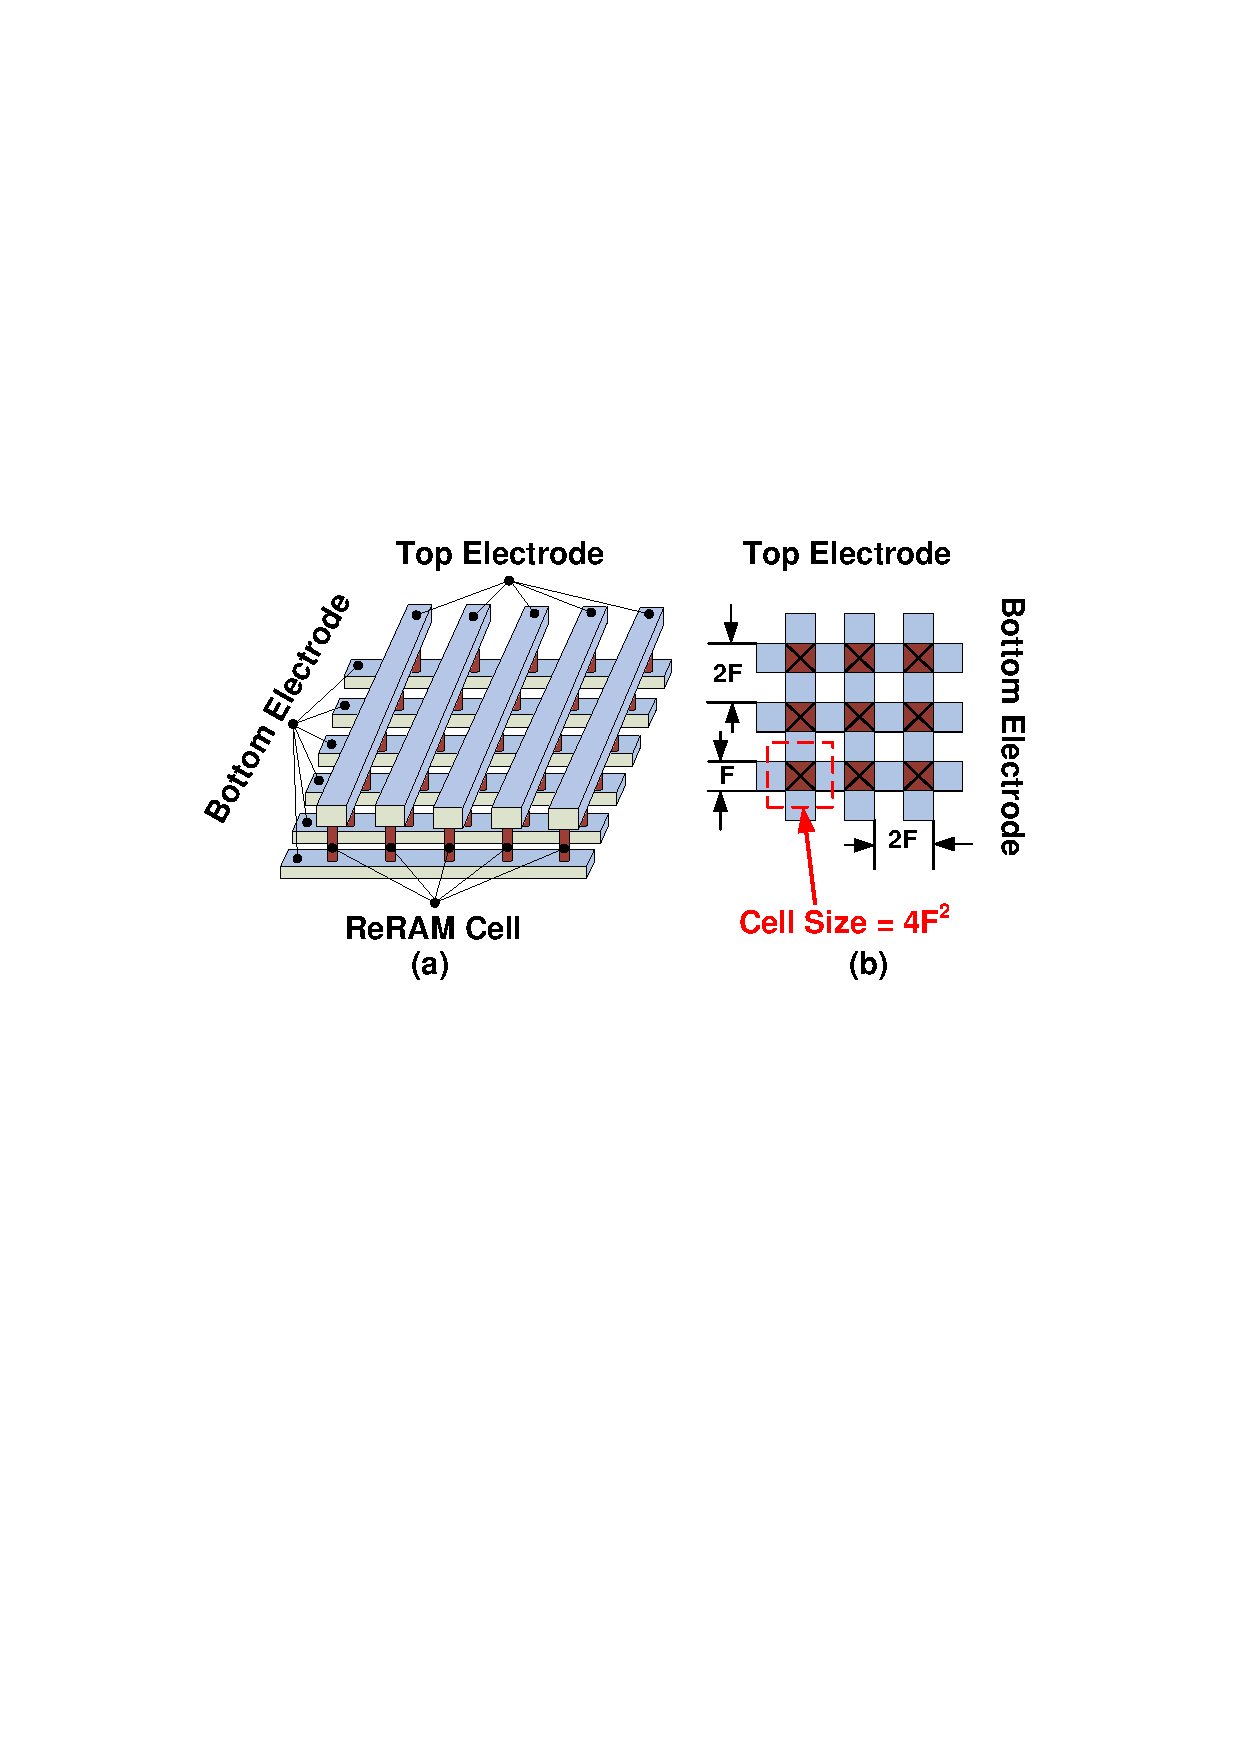
\includegraphics[width=0.45\textwidth]{./figures/crossbar_array2.pdf}\\\vspace{-10pt}
  \caption{A schematic view of a typical cross-point array. (a) The perspective of the cross-point array.
  (b) The top view of the array, from which we can clearly see that the size of each cell is $4F^2$. }\label{fig:array}
\vspace{-12pt}
\end{figure}

There are several write/read schemes for cross-point ReRAM arrays. For
example, the write operation can write either a single-bit per access or
several bits attached to the same wordline at the same time. Although the second
scheme has higher bandwidth, it requires a two-step write operation to
prevent unintentional writing~\cite{memristor:Cong}, which significantly
increases the write latency.
%Therefore, the write latency for the multi bit write operation is much larger than the one bit operation.
Furthermore, while writing to a cross-point array, the unselected wordlines
and bitlines can be either left floating or half-biased. In contrast, while reading
a cell, the selected wordline should be biased with a read
voltage and all the other wordlines and bitlines in the array are shunted
to ground. The current in each bitline is then sensed and compared to a
reference current to determine the cell content. However, due to the sneak
current existing in the cross-point array, the current in bitlines also
varies depending upon the data patterns of unselected cells.
%is impacted significantly by the data pattern of the unselected cells in the array.
This read disturbance restricts the size of a cross-point array, since
sneak current increases as the number of cells attached to wordlines and
bitlines increases, which makes it difficult to sense the current
difference of the selected cell at HRS and LRS. Besides, the existence of
the voltage drop along the nanowires also limits the length of wordlines
and bitlines. Therefore, a cross-point array should be sized carefully to
meet the requirements of the read/write reliability.
%Therefore, a cross-point array should be sized carefully such that the current difference of the selected cell at HRS and LRS is large enough for reliable sensing.
In addition to all of these write/read schemes, different cell parameters
will also impact the reliability, energy consumption, bandwidth, and area
efficiency of the cross-point ReRAM array. In this case, it is not
straightforward for a designer to figure out how to design a workable
memory array with the minimum energy consumption and area overheads. Thus,
the following sections will propose a worst-case oriented methodology to
help designers make decisions early in the design flow.

%Depending upon the read/write scheme, the size of the array can vary significantly. In this work, we propose a methodology to find the minimum array size that meets specific energy and area constraints based on the worst-case state of the array. This will help designers find an optimal memory organization early in the design flow. %t read/write schemes as well as array sizes can be chosen for the cross-point array, it is not straightforward to figure out how to design a workable memory array with the minimum energy consumption and area overheads. Thus, following sections will proposed a worst-case oriented methodology to help designer make the decision early in the design flow.


%\subsection{Limitations of Cross-Point Architecture}
%\subsection{Related Work and Motivations}
%Although the cross-point structure can provide the fabricate simplicity and area efficiency, it also incur lots of design challenges. Many of the design challenges, such as the array size, resistance ratio as well as the data pattern have been presented and analyzed by previous researches. However, all of these researches focus on the cross point array itself and do not take into account the area or energy overhead of the peripheral circuit. Besides, a comprehensive study on different write/read schemes is also lacking. In this
%
%
%One of the well known design challenge of cross-point is the sneak path existed in the memory array, which will lead a read failure during the read operation and bring in extra energy consumption. Besides, there are also several design options can be chose during the system design. Following shows an example, which shows part of the design challenges of the cross-point structure motivates the work in this paper.
%\begin{enumerate}
%  \item \textbf{Example of the Design Challenges of Cross-Point Structure.}\\
%  In order to
%
%\begin{figure}
%\centering
%  % Requires \usepackage{graphicx}
%  \includegraphics[width=0.4\textwidth]{./figures/example1_large.pdf}\\
%  \caption{Case 1: Voltage Drop Along the Word Line during Write Operation.}\label{fig:exampl1}
%\end{figure}
%
%  \item \textbf{Read Margin Disturbance}\\
%  123
%  \item \textbf{Energy Waste Due to Sneak Pass}\\
%  123
%\end{enumerate}
%
%~\cite{crossbar_NANO08_Nauenheim}~\cite{memristor:analog}~\cite{moore}
%
\vspace{-5pt}
\subsection{Modeling of the Cross-Point Memory}\label{sec:model}

%\subsection{Basic model of Cross-Point Memory}
The basic circuit model of an $M$ by $N$ cross-point ReRAM array is shown
in Figure~\ref{fig:modeling}. This model is built upon Kirchhoff's Current
Law (KCL) and its validity can be guaranteed by deductions from basic
circuit theory. The horizontal lines are wordlines and the vertical lines
represent bitlines. The ReRAM cells are located at each wordline and
bitline cross-point. A detailed cross-point structure is also shown in
Figure~\ref{fig:modeling}(b). The resistance of the ReRAM cell at the
cross-point of $i^{th}$ wordline and $j^{th}$ bitline is represented by
$R_{i,j}$. We assume the resistance of the wire connecting two
cross-points to be $R_{line}$. The input resistance of each wordline or
bitline driver is $R_v$ and the resistance of a sense amplifier is $R_s$.
In order to set up the KCL equations, the voltage at each cross-point is
indicated as $V_{i,j}$ for the wordline layer and $V'_{i,j}$ for the
bitline layer. In addition, the input voltage for the $i^{th}$ wordline is
$V_{Wi}$ and for the $i^{th}$ bitline is $V_{Bi}$. In the case that a
wordline is driven from both sides, the voltage at the other end of the
$i^{th}$ wordline is represented as $V'_{Wi}$.

%Finally, the voltage at the sense amplifier is $V'_{Bi}$ during the read operation.
%YOU MIGHT WANT TO CHANGE THE ABOVE PARA INTO A TABLE

\begin{figure}%[!hb]
\centering
  % Requires \usepackage{graphicx}
  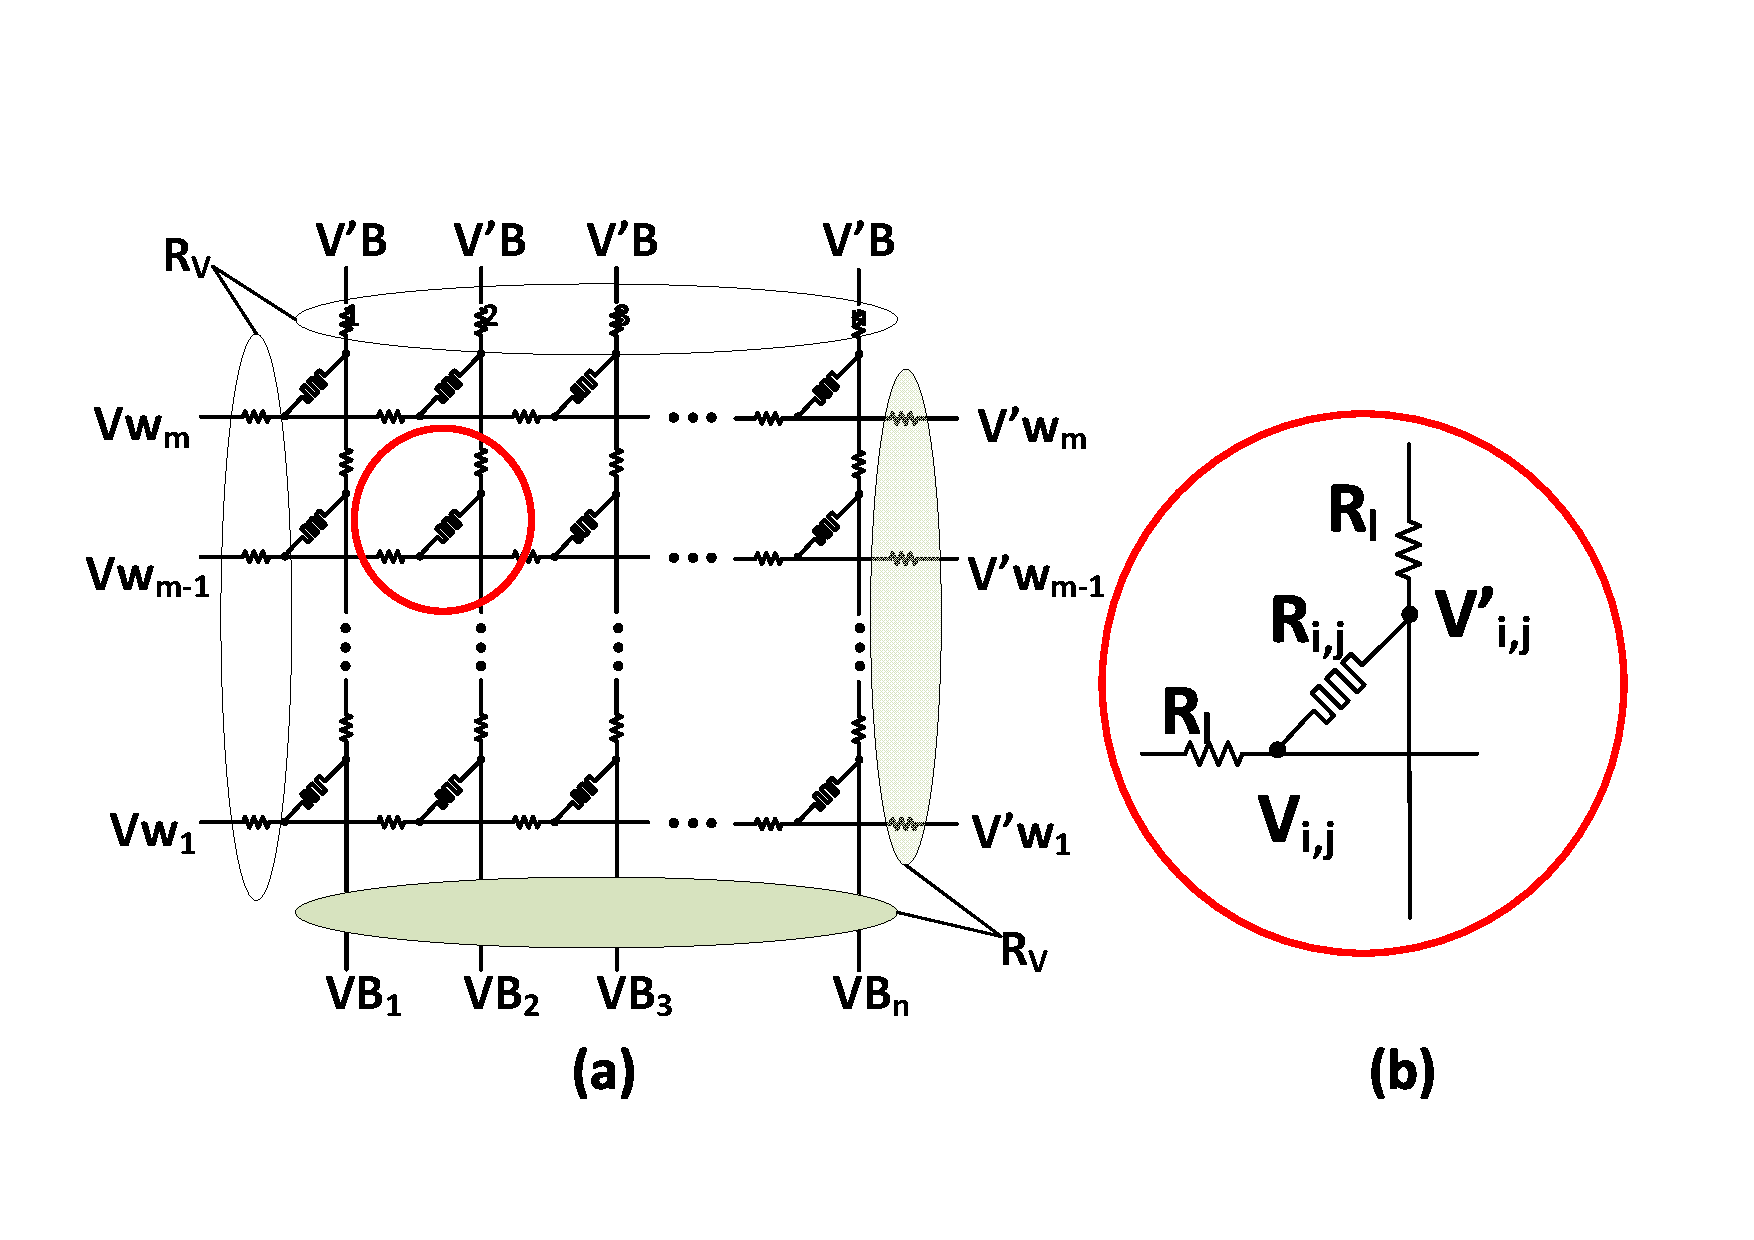
\includegraphics[width=0.45\textwidth]{./figures/model_f.pdf}\\
  \vspace{-8pt}
  \caption{The circuit model of the cross-point array.}\label{fig:modeling}
  \vspace{-4pt}
\end{figure}

%\subsection{Mathematical Model of a Cross-Point Array}
Based on this model, the current equations for each cross-point can be
obtained. All of the cross-points have similar structure with no more than
three current branches, and therefore it is very easy to set up the KCL
equations for each cross-point. Since the cross-points at the edges of the
array have different write/read conditions, the KCL equations of these
cross-point should be adjusted according to each write/read scheme.All of
the KCL equations can be considered as a system of linear equations, which
has the following form of {$ A\cdot~V~=~C $}, where $A$ is a
${2mn\times{2mn}}$ coefficient matrix and $C$ is a ${2mn\times{1}}$
vector, containing the constant terms of these equations. Thus, with
parameters such as the resistance of ReRAM cells, the resistance of
interconnect wires, program voltages, and write/read schemes, voltages at
various cross points can be obtained by solving the system of linear
equations. With detailed voltage values, $V_{2mn{\times}1}$, we can
analyze the array at a fine granularity. These values are also critical to
evaluate the reliability, energy consumption, driven current density, and
area overheads of a cross-point array.

To validate the analytical model, we compare the results with
HSPICE~\cite{HSPICE} simulations using a resistor model in cross-point
memory arrays. The results of eight cross-point arrays with different
array sizes and specific data patterns are shown in
Figure~\ref{fig:validation}, which shows that the voltage drop on the
selected cell derived from our analytical model are consistent with the
HSPICE simulation results.
\begin{figure}%[!t]
\centering\label{fig:SPICE}
  % Requires \usepackage{graphicx}
  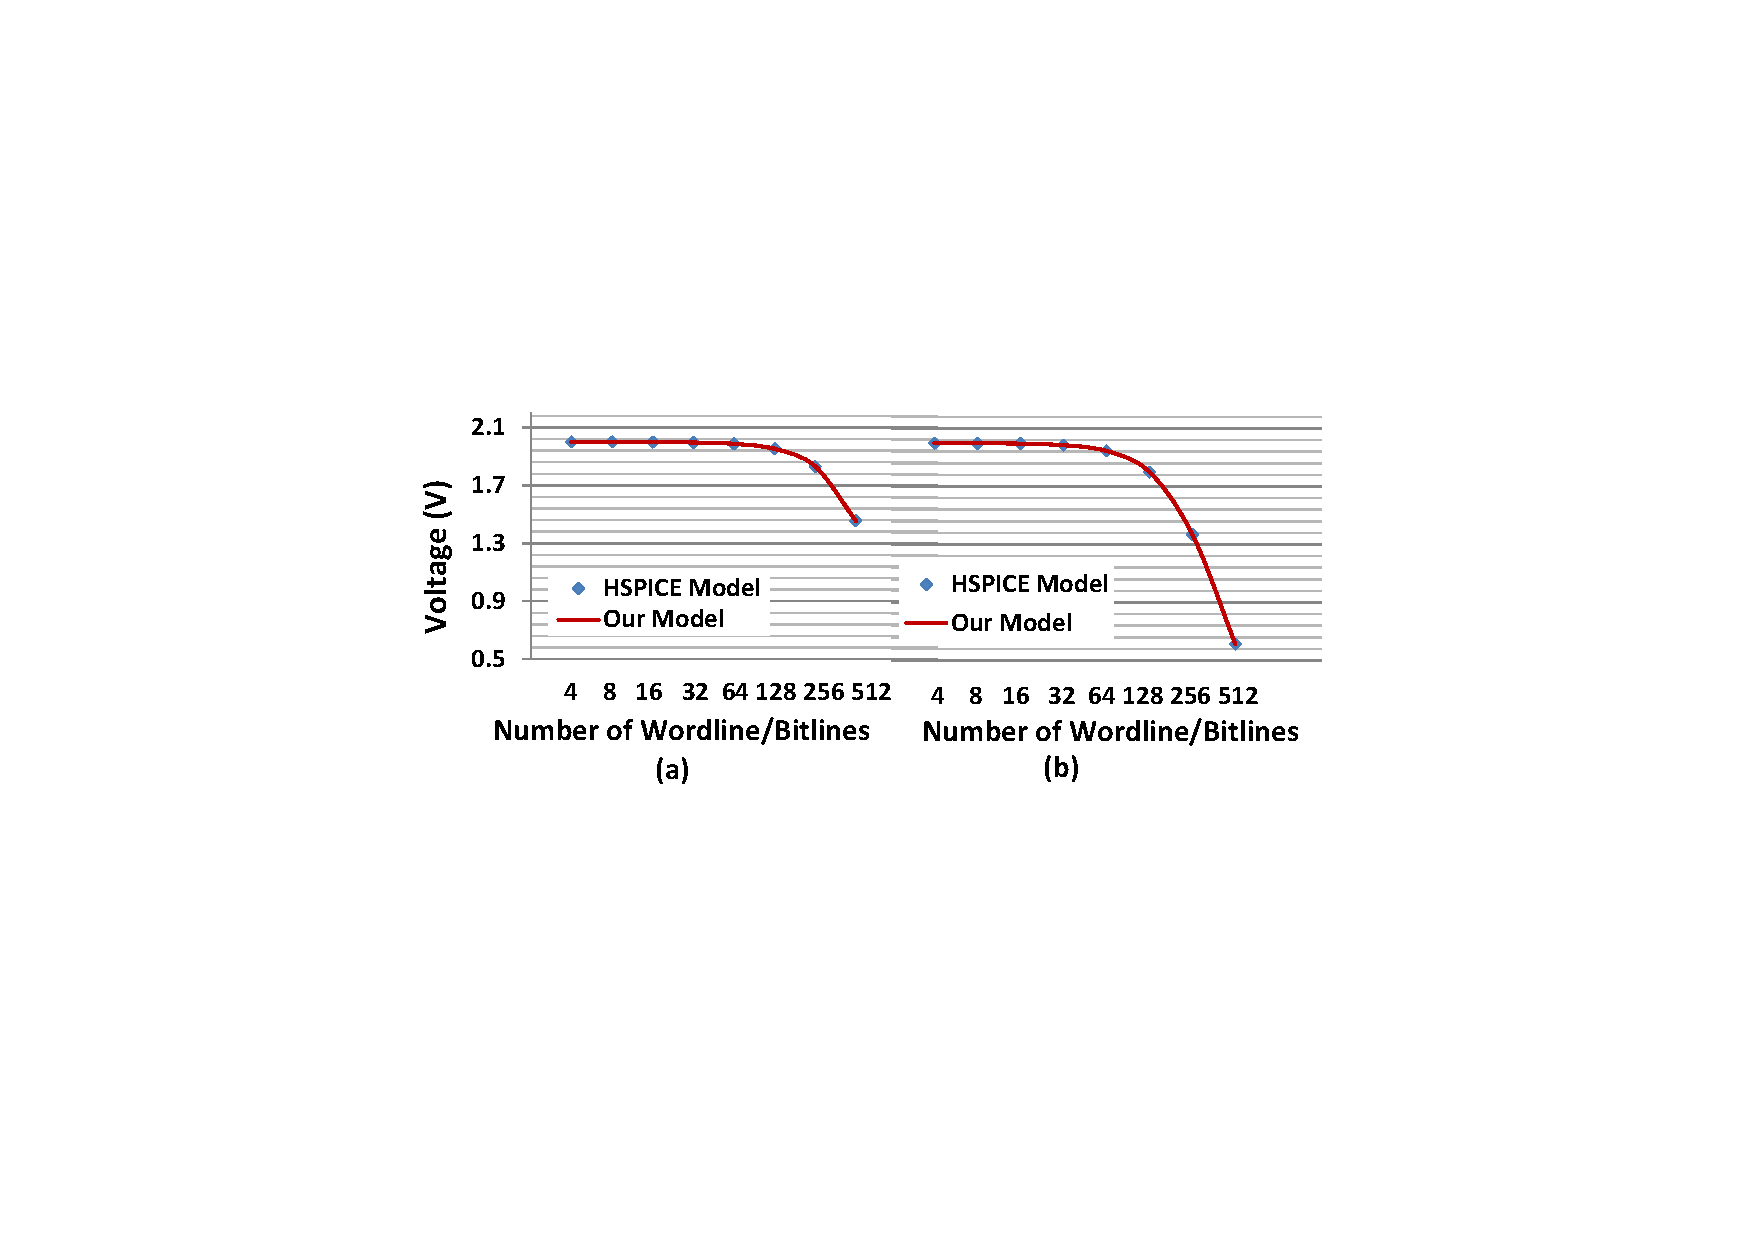
\includegraphics[width=0.5\textwidth]{./figures/SPICE1.pdf}\\
  \caption{Validation of the analytical model against SPICE simulation. The two figures show the voltage drops obtained from our model and SPICE (a) with a nonlinearity factor of 5 and (b) without nonlinearity.}\label{fig:validation}
    \vspace{-10pt}
\end{figure}
%
%The characteristics of the linear system can be summarized as:
%\begin{enumerate}
%  \item
%  As shown in Equation~(\ref{equ:blockedmatrix}), the coefficient matrix $A$ can be further partitioned into 4 smaller subblocks :
%    \begin{equation}\label{equ:blockedmatrix}
%        \mathbf{A} = \left[
%        \begin{array}{cc}
%            A1 & A2  \\
%            A3 & A4  \\
%        \end{array} \right].
%    \end{equation}
%All of these subblocks have the same size of $m\times n$. Subblock
%$A2$ and $A3$ are diagonal matrixes and have the value of: $A2_{i,i} =
%A3_{i,i} = R_{i,i}^{-1}$. $A2$ and $A3$ do not change their values
%with different schemes. However, $A1$ and $A4$ are a little more
%complex than $A2$ and $A3$. $A1$ is a tridiagonal matrix and has
%nonzero elements only in the main diagonal, and the first line below
%and above the diagonal. Similarly, $A_4$ is a special tridiagonal
%matrix, which has nonzero elements in the main diagonal, and the
%$n^{th}$ line below and above the diagonal, where $n$ is the number of
%bitline in the cross-point model. The value of the elements in $A1$
%and $A4$ can be easily derived from Equation (\ref{equ:KCL1}) and
%(\ref{equ:KCL2}). However, the edge condition varies with different
%program schemes. Therefore, the coefficients related to the edge
%condition should be set according to the program schemes. Clearly, the
%four edges shown in Figure~\ref{fig:modeling} correspond to different
%coefficients in $A1$ and $A4$. Due to the space limitations, we
%consider the nodes at the left edge of the array as an example. A
%similar procedure can be followed to initiate the coefficients of
%other edge. The coefficients of nodes at the left edge of the array
%($V_{i,1}$) can be set as:
%
%    \begin{equation}
%    A1(k,k) = \left\{
%    \begin{array}{ll}
%    -(R_l^{-1}+R_{i,1}^{-1})   & \text{if } floating\\
%    -(R_v^{-1}+R_l^{-1}+R_{i,1}^{-1})& \text{if } activated
%    \end{array} \right.
%    \end{equation}
%    where $k=(n-1)i+1$ for $i=1,2...m$.
%
%  \item The constant terms $C$ is a $2mn{\times}1$ vector. Equation(\ref{equ:KCL1})-(\ref{equ:KCL4}) show that only KCL equations of the activated points have constant terms. Therefore, only the following elements in $C$ may have non-zero value: $C((i-1)n+1)$, $C(in)$, $C(mn+i)$ and $C((2m-1)n+i)$ for $i=1,2...m$, corresponding to the nodes at the four edges respectively. Likewise, as an example, we consider nodes $V_{i,1}$. The constant corresponding to these nodes can be defined as:
%    \begin{equation}
%    C((i-1)n+1) = \left\{
%    \begin{array}{ll}
%    0   & \text{if } floating\\
%    -R_v^{-1}V_{Wi}& \text{if } activated
%    \end{array} \right.
%    \end{equation}
%\end{enumerate}

%%\vspace{10pt}
\section{Modeling of the Cross-Point Memory}\label{sec:model}

%In this section, we present a detailed mathematical model for cross-point
%arrays. By using this model, along with specific parameters and edge
%conditions, the reliability, energy consumption, and area overheads of
%different read/write schemes can be easily evaluated.
In this section, we present a brief introduction of mathematical model of
the cross-point array. More details can be found in the Appendix.

%\subsection{Basic model of Cross-Point Memory}
The basic circuit model of an $M$ by $N$ cross-point ReRAM array is shown
in Figure~\ref{fig:modeling}. This model is built upon Kirchhoff's Current
Law (KCL) and its validity can be guaranteed by deductions from basic
circuit theory. The horizontal lines are wordlines and the vertical lines
represent bitlines. The ReRAM cells are located at each wordline and
bitline cross-point.

A detailed cross-point structure is also shown in
Figure~\ref{fig:modeling}(b). The resistance of the ReRAM cell at the
cross-point of $i^{th}$ wordline and $j^{th}$ bitline is represented by
$R_{i,j}$. We assume the resistance of the wire connecting two
cross-points to be $R_{line}$. The input resistance of each wordline or
bitline driver is $R_v$ and the resistance of a sense amplifier is $R_s$.
In order to set up the KCL equations, the voltage at each cross-point is
indicated as $V_{i,j}$ for the wordline layer and $V'_{i,j}$ for the
bitline layer. In addition, the input voltage for the $i^{th}$ wordline is
$V_{Wi}$ and for the $i^{th}$ bitline is $V_{Bi}$. In the case that a
wordline is driven from both sides, the voltage at the other end of the
$i^{th}$ wordline is represented as $V'_{Wi}$.

%Finally, the voltage at the sense amplifier is $V'_{Bi}$ during the read operation.
%YOU MIGHT WANT TO CHANGE THE ABOVE PARA INTO A TABLE

\begin{figure}%[!hb]
\centering
  % Requires \usepackage{graphicx}
  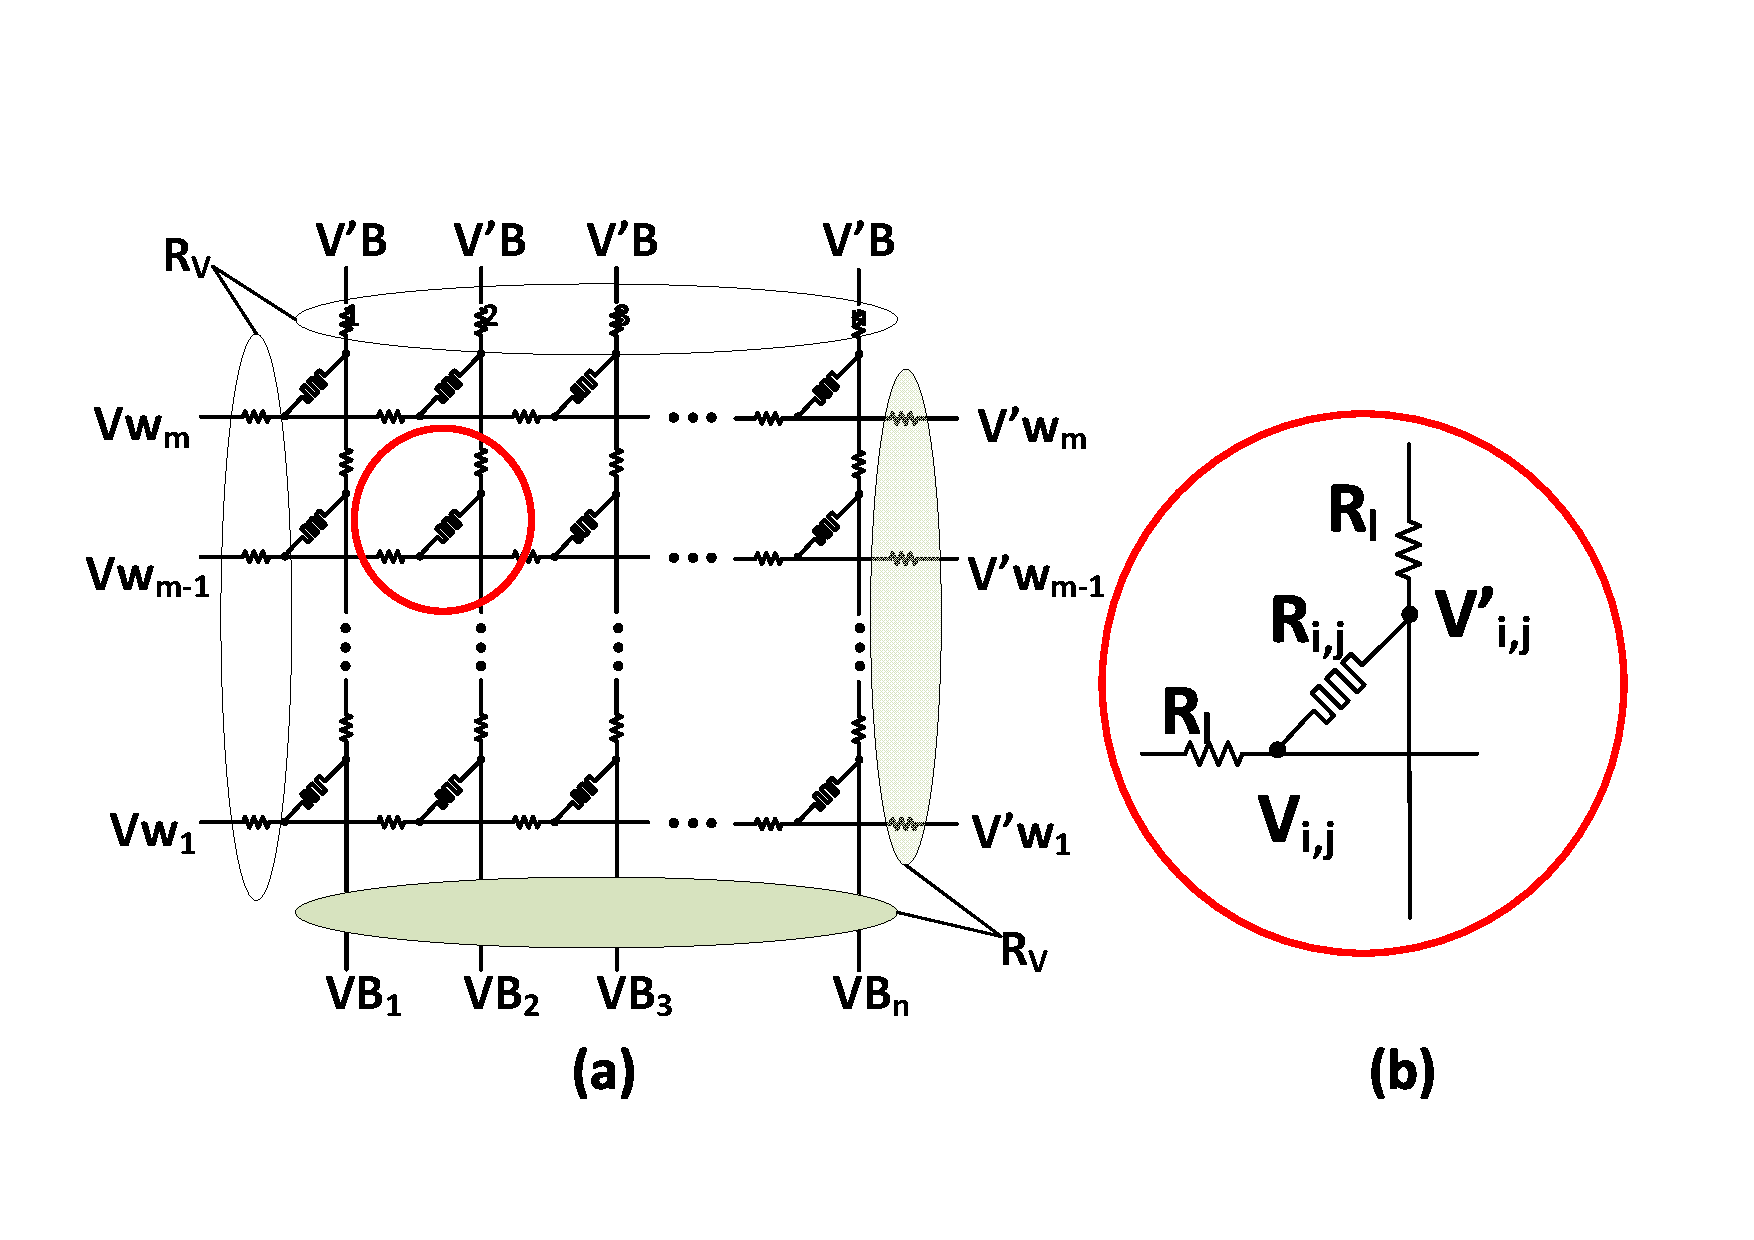
\includegraphics[width=0.45\textwidth]{./figures/model_f.pdf}\\
  \caption{The circuit model of the cross-point array.}\label{fig:modeling}
  \vspace{-12pt}
\end{figure}

%\subsection{Mathematical Model of a Cross-Point Array}
Based on this model, the current equations for each cross-point can be
obtained. All of the cross-points have similar structure with no more than
three current branches, and therefore it is very easy to set up the KCL
equations for each cross-point.

However, it is important to note that KCL equations for cross-points at
the edges of the array vary with different write/read schemes. For
example, the unselected wordline for write operation can be either half
biased or left floating. Thus, the edge conditions should be adjusted
according to each write/read scheme. In particular, according to their
locations and write/read schemes, all of the cross-points in an array can
be classified into three major categories: \emph{normal point},
\emph{activated point} and \emph{floating point}. The normal points are
located inside the memory array. The activated point and floating point
represent the nodes at the edge of cross-point array with different
conditions: an edge point, which is directly connected to the voltage
input or to the ground, can be considered as an activated point.
Otherwise, it is a floating point. The detailed models for these points
can be found in the Appendix. All of the KCL equations can be considered as a system of linear equations, which has the following form
\begin{equation}\label{equ:matrix}
A\cdot V = C,
\end{equation}
where $A$ is a ${2mn\times{2mn}}$ coefficient matrix and $C$ is a
${2mn\times{1}}$ vector, containing the constant terms of these equations.
We demonstrate that all of the KCL equations have simple and similar
structures. Therefore, the linear equation system has a relatively fixed
format and simple structure, making it easy to establish and adjust the
coefficients and constants according to different design schemes. Besides,
due to the simplicity of the KCL equation, $A$ is populated primarily with
zeros and can be saved as a sparse matrix, which will further reduce the
storage cost during the computation.

To validate our analytical model, we compare the results with
HSPICE~\cite{HSPICE} simulations using a resistor model in cross-point
memory arrays. DC analysis was performed by HSPICE which solved the
voltage of every node in the array. The results of eight cross-point
arrays with different array sizes and specific data patterns are shown in
Figure~\ref{fig:validation}, which shows that the voltage drop on the
selected cell derived from our analytical model are consistent with the
HSPICE simulation results.
\begin{figure}%[!t]
\centering\label{fig:SPICE}
  % Requires \usepackage{graphicx}
  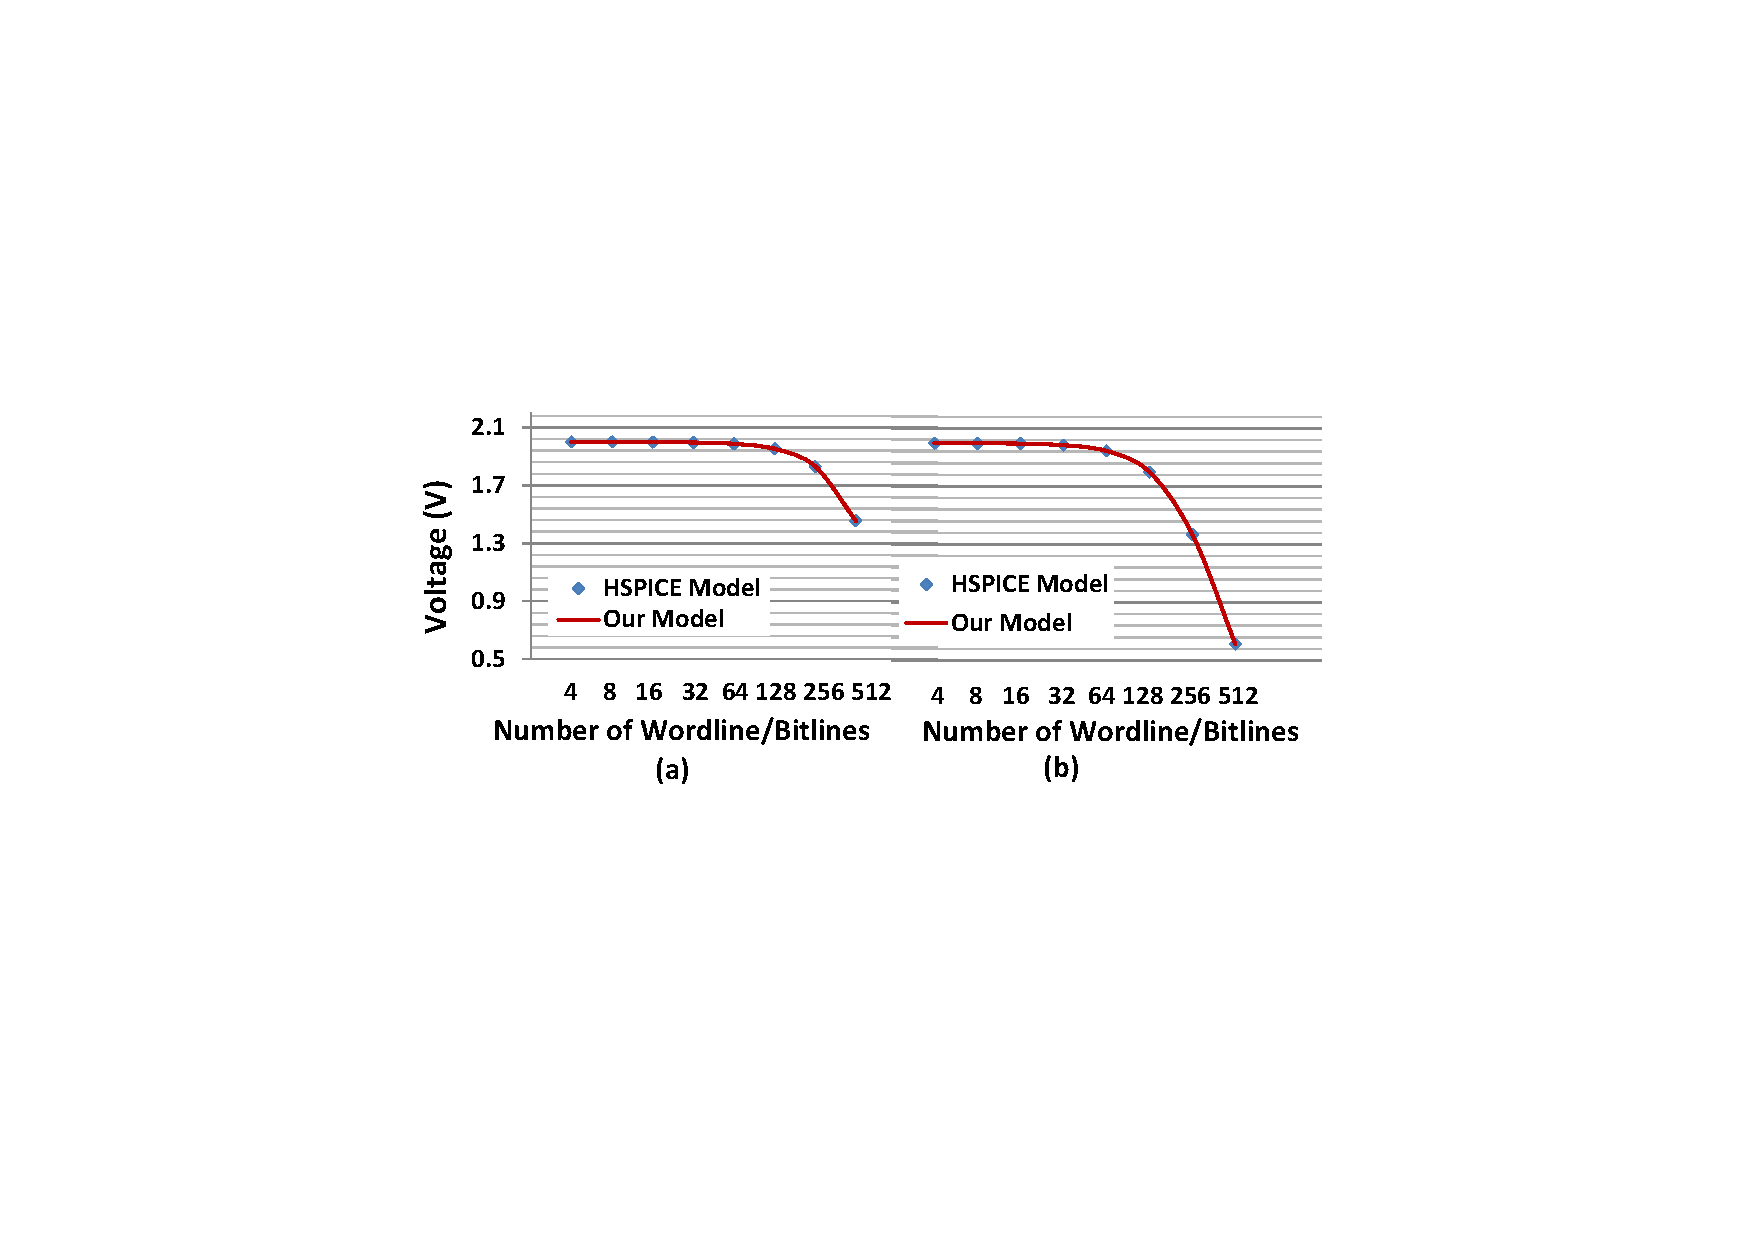
\includegraphics[width=0.5\textwidth]{./figures/SPICE1.pdf}\\
  \caption{Validation of the analytical model against SPICE simulation. The two figures show the voltage drops obtained from our model and SPICE (a) with a nonlinearity factor of 5 and (b) without nonlinearity.}\label{fig:validation}
    \vspace{-10pt}
\end{figure}
%
%The characteristics of the linear system can be summarized as:
%\begin{enumerate}
%  \item
%  As shown in Equation~(\ref{equ:blockedmatrix}), the coefficient matrix $A$ can be further partitioned into 4 smaller subblocks :
%    \begin{equation}\label{equ:blockedmatrix}
%        \mathbf{A} = \left[
%        \begin{array}{cc}
%            A1 & A2  \\
%            A3 & A4  \\
%        \end{array} \right].
%    \end{equation}
%All of these subblocks have the same size of $m\times n$. Subblock
%$A2$ and $A3$ are diagonal matrixes and have the value of: $A2_{i,i} =
%A3_{i,i} = R_{i,i}^{-1}$. $A2$ and $A3$ do not change their values
%with different schemes. However, $A1$ and $A4$ are a little more
%complex than $A2$ and $A3$. $A1$ is a tridiagonal matrix and has
%nonzero elements only in the main diagonal, and the first line below
%and above the diagonal. Similarly, $A_4$ is a special tridiagonal
%matrix, which has nonzero elements in the main diagonal, and the
%$n^{th}$ line below and above the diagonal, where $n$ is the number of
%bitline in the cross-point model. The value of the elements in $A1$
%and $A4$ can be easily derived from Equation (\ref{equ:KCL1}) and
%(\ref{equ:KCL2}). However, the edge condition varies with different
%program schemes. Therefore, the coefficients related to the edge
%condition should be set according to the program schemes. Clearly, the
%four edges shown in Figure~\ref{fig:modeling} correspond to different
%coefficients in $A1$ and $A4$. Due to the space limitations, we
%consider the nodes at the left edge of the array as an example. A
%similar procedure can be followed to initiate the coefficients of
%other edge. The coefficients of nodes at the left edge of the array
%($V_{i,1}$) can be set as:
%
%    \begin{equation}
%    A1(k,k) = \left\{
%    \begin{array}{ll}
%    -(R_l^{-1}+R_{i,1}^{-1})   & \text{if } floating\\
%    -(R_v^{-1}+R_l^{-1}+R_{i,1}^{-1})& \text{if } activated
%    \end{array} \right.
%    \end{equation}
%    where $k=(n-1)i+1$ for $i=1,2...m$.
%
%  \item The constant terms $C$ is a $2mn{\times}1$ vector. Equation(\ref{equ:KCL1})-(\ref{equ:KCL4}) show that only KCL equations of the activated points have constant terms. Therefore, only the following elements in $C$ may have non-zero value: $C((i-1)n+1)$, $C(in)$, $C(mn+i)$ and $C((2m-1)n+i)$ for $i=1,2...m$, corresponding to the nodes at the four edges respectively. Likewise, as an example, we consider nodes $V_{i,1}$. The constant corresponding to these nodes can be defined as:
%    \begin{equation}
%    C((i-1)n+1) = \left\{
%    \begin{array}{ll}
%    0   & \text{if } floating\\
%    -R_v^{-1}V_{Wi}& \text{if } activated
%    \end{array} \right.
%    \end{equation}
%\end{enumerate}
Thus, with parameters such as the resistance of ReRAM cells, the
resistance of interconnect wires, program voltages, and write/read
schemes, voltages at various cross points can be obtained by solving the
system of linear equations. With detailed voltage values,
$V_{2mn{\times}1}$, we can analyze the array at a fine granularity. These
values are also critical to evaluate the reliability, energy consumption,
driven current density, and area overheads of a cross-point array.

\vspace{-4pt}
\section{Analysis of Design Constraints - A Case Study}\label{sec:w_and_r}

In this section, we study the effect of various schemes on cross-point
ReRAM arrays in detail. Specifically, we evaluate the design constraints
on array size, energy consumption and area overhead in worst case
scenarios. The results of this study will be useful when designing a
cross-point array.

\vspace{-10pt}
\subsection{Overview}
%As shown in Figure~\ref{fig:modeling}, i
In order to write or read a cross-point array, proper voltages should be
applied across the ReRAM cell. Although the goal of a read operation is
different from a write operation, both of them are realized by fully
biasing the selected wordlines/bitlines and floating (or half biasing)
unselected wordlines/bitlines. Thus, the coefficient matrix $A$ and the
constant vector $C$ are very similar for both. In addition, their energy
consumption and area overhead will also have a similar trend. Therefore,
in this section, we first study the write operation comprehensively. After
that, for read operation, we mainly focus on the read margin analysis
since it is unique for read operations.
%can be very useful to guide the design of the cross-point array.
%Also, we assumes that the in the case of worst scenario, the ReRAM cells at the selected wordline, th
%Since it is impossible to consider all of the data pattern stored in the array,

Table~\ref{table:parameter} shows the circuit parameters of our baseline
50nm design. The data is derived from the recently published studies on
ReRAM~\cite{ReRAM_overview,memristor:Cong,ReRAM_Renesas}. The nonlinearity
coefficient is defined as
\begin{equation}
K_r(p,V) = p \times R(V/p)/R(V),
\end{equation}
where $R(V/p)$ and $R(V)$ are the equivalent resistance of the cell biased
at $V/p$ and $V$~\cite{memristor:Cong}. Therefore, the resistance of a
ReRAM cell with nonlinearity is not constant but varies with the applied
voltage. For example, for a ReRAM cell with nonlinearity of 20, the
resistance of half biased cell is 10 times larger than resistance of fully
biased cell. By using these parameters, we study reliability, energy
consumption, and area overheads for four different write schemes, and
discuss the sensitivities of these schemes to the data pattern of HRS and
LRS ReRAM cells and cell nonlinearity. In this section, the baseline
design uses a cell with write current of $40 uA$ and nonlinearity $Kr=20$.
A sensitivity study varying the nonlinearity coefficient and the write
current is presented in Section~\ref{sec:scale}.

\begin{table}[!t]
  \centering
  \scriptsize
    \scriptsize
  \caption{Parameters of the baseline Cross-Point Array}\label{table:parameter}
  \vspace{-5pt}
%  \begin{tabular}{|cccccp{3.5cm}|}
  \begin{tabular}{c|c|c}
    \hline    \hline
    % after \\: \hline or \cline{col1-col2} \cline{col3-col4} ...
    \textbf{Metric} & \textbf{Description} & \textbf{Typical Values (Range)} \\
    \hline
    \textbf{$A_{cell}$} & Cell Size & \textbf{$4F^2$} \\
    \textbf{$R_l$} &  Interconnection Resistance&\textbf{$0.65\Omega$} \\
    \textbf{$V_{RESET}$} & Threshold voltage for RESET&\textbf{$2.0V$} \\
    \textbf{$V_{SET}$} & Threshold voltage for SET&\textbf{$-2.0V$} \\
    \textbf{$V_{READ}$} & Read Voltage of Cell&\textbf{$0.5V$} \\
    \textbf{$I_{on}$} & Write Current for LRS Cell &\textbf{$40uA$~~($40\sim200uA$)} \\
    \textbf{$V_{W}(R)$} & Wordline Voltage during Read &\textbf{$0.5V$} \\
    \textbf{$V_{W}(W)$} & Wordline Voltage during Write  &\textbf{$\pm2V$} \\
    \textbf{$V_{W}(H)$} & Half Selected wordline Voltage &\textbf{$1V$} \\
    \textbf{$V_{B}(R)$} & Bitline Voltage during Read  &\textbf{$0V$} \\
    \textbf{$V_{B}(W)$} & Bitline Voltage during Write  &\textbf{$0V$} \\
    \textbf{$V_{B}(H)$} & Half Selected bitline Voltage &\textbf{$1V$} \\
    \textbf{$K_r$} & Nonlinearity of ReRAM Cell &\textbf{$20$~~($2\sim40$)} \\
    \textbf{$M,N$} & Number of wordlines/bitlines &\textbf{$512$~~($8\sim1024$)} \\
    \hline
  \end{tabular}
  \vspace{-10pt}
\end{table}

\subsection{Write Operation}
To write a ReRAM cell, an external voltage is applied across the cell for
a certain duration. Intuitively, there are four possible schemes for the
write operation: \emph{FWFB} scheme activates the selected wordline and
selected bitline, and leaves all of other lines floating; \emph{FWHB}
scheme activates the selected wordline and bitline, leaves all the
unselected wordlines floating, and half biases the unselected bitlines;
\emph{HWFB} scheme activates the selected wordline and bitline, leaves all
the unselected bitlines floating, and half biases the unselected
wordlines; \emph{HWHB} scheme activates the selected wordline and bitline,
and half biases the unselected wordlines and bitlines. However, the FWFB
scheme has an inherent problem that may result in severe write
disturbance~\cite{crossbar_NANO2003_Ziegler}. Therefore, in the following
discussion, we only compare the results of the FWHB, HWFB and HWHB
schemes. For each of these three schemes, we can either write several
cells on one wordline at the same time (multi-bit write) or write only one
bit per access (single-bit write) and distribute the write operation to
several arrays.
%Since several potential read/write schemes can be used to program a memory array, it is difficult to identify the ideal scheme that meets the design constraints in terms of area, energy, and reliability.
%However, the FWFB scheme has inherent problem that may result in severe
%write disturbance. For example, for writing a ReRAM cell located at the
%cross point of the $i^{nd}$ wordline and the $j^{nd}$ bitline in a $M
%\times N$ matrix ($M>N$), the worst case voltage drop of unselected cells
%appears when all of the ReRAM cells at the selected bitline are in the
%HRS, while all of the other cells are in the LRS. In this case, the
%voltage drop across the selected cell almost has the same magnitude as the
%unselected cell at the same bitline, resulting the write disturbance to
%all of the unselected cells at the selected bitline. Actually, the worst
%case voltage drop of the unselected cell can be calculated as:
%\begin{equation}\label{worst_FWFB}
%V_{worst}=V_{select} \cdot [1-\frac{1}{M+(N-1)R_{off}/R_{on}}].
%\end{equation}
%Considering that the reported On-OFF resistance ratio of ReRAM cell is
%always $>50$
%~\cite{ReRAM_IEDM2010_Ho,ReRAM_IEDM2010_Chien,ReRAM_IEDM2010_Lee_Diode,ReRAM_IEDM2010_Lee_Evidence,ReRAM_ISSCC2011_Sheu,ReRAM_ISSCC2011_Otsuka},
%, the worst case voltage drop at the unselected cell is larger than $98\%$
%of the voltage at the selected cell, making it is impossible to build a
%reliable cross-point structure ReRAM with the FWFB scheme. Therefore, in
%the following discussion, we only compare the results of FWHB, HWFB and
%HWHB schemes. For each of these three schemes, we can either write several
%cells at one wordline at the same time or only write one bit per access
%and distribute the write operation to several arrays. In the following
%discussion, we start from one bit per access write operation, then the
%results of one wordline per access method are discussed.

%Since reliability, energy consumption, and area overheads for these
%schemes are different, we address these problems separately and finally
%combine all constraints to provide design guidelines for write operations.


\vspace{5pt}\noindent\textbf{Reliable Write Operations.} Write reliability
is a serious concern in cross-point arrays. In an ideal condition, the
resistance of wires and the sneak currents in unselected cells are
negligible. In such a scenario, all the write schemes discussed above can
make sure that the write voltage $V_W(W)-V_B(W)$ is fully applied across
the specified cell. However, in reality, both wire resistance and sneak
current are non-trivial. Hence, the voltage applied across a cross-point
varies based on the location of the cell as well as the data pattern
stored in all of the ReRAM cells in the array. A write is considered
reliable if it modifies the content of the selected cells to the new value
without disturbing other unselected cells. Correspondingly, there are two
potential problems with writes: \emph{write failure}, an unsuccessful
write on selected cells, and \emph{write disturbance}, an undesirable
write to unselected cells. It is necessary to ensure that a write scheme
guarantees reliable operation even in the worst case (w.r.t the location
of cells to written and the data pattern stored in the cross-point array).

%We first use an example to show the problem with FWFB scheme, which may
%result in severe write disturbance. Figure~\ref{fig:FWFR} shows the
%voltage drop across each ReRAM cell of a $64 \times 64$ cross-point array.
%In this example, in order to write the cell at the cross point of the
%$32^{nd}$ wordline and the $32^{nd}$ bitline, the selected wordline and
%bitline are biased at 2V and 0V, respectively. All of the other wordlines
%and bitlines are left floating. The ReRAM cells at the selected bitline are
%in the HRS, while all of the other cells are in the LRS. It is clear that
%the voltage drop across the selected cell ($V_{32,32}$) almost has the
%same magnitude as the unselected cell at the same bitline, resulting the
%write disturbance to all of the unselected cells at the selected bitline.
%Actually, for a $M \times N$ matrix ($M>N$), the worst case voltage drop
%of the unselected cell can be calculated as:
%\begin{equation}\label{worst_FWFB}
%V_{worst}=V_{select} \cdot [1-\frac{1}{M+(N-1)R_{off}/R_{on}}].
%\end{equation}
%
%\begin{figure}[!b]
%\centering
%  % Requires \usepackage{graphicx}
%  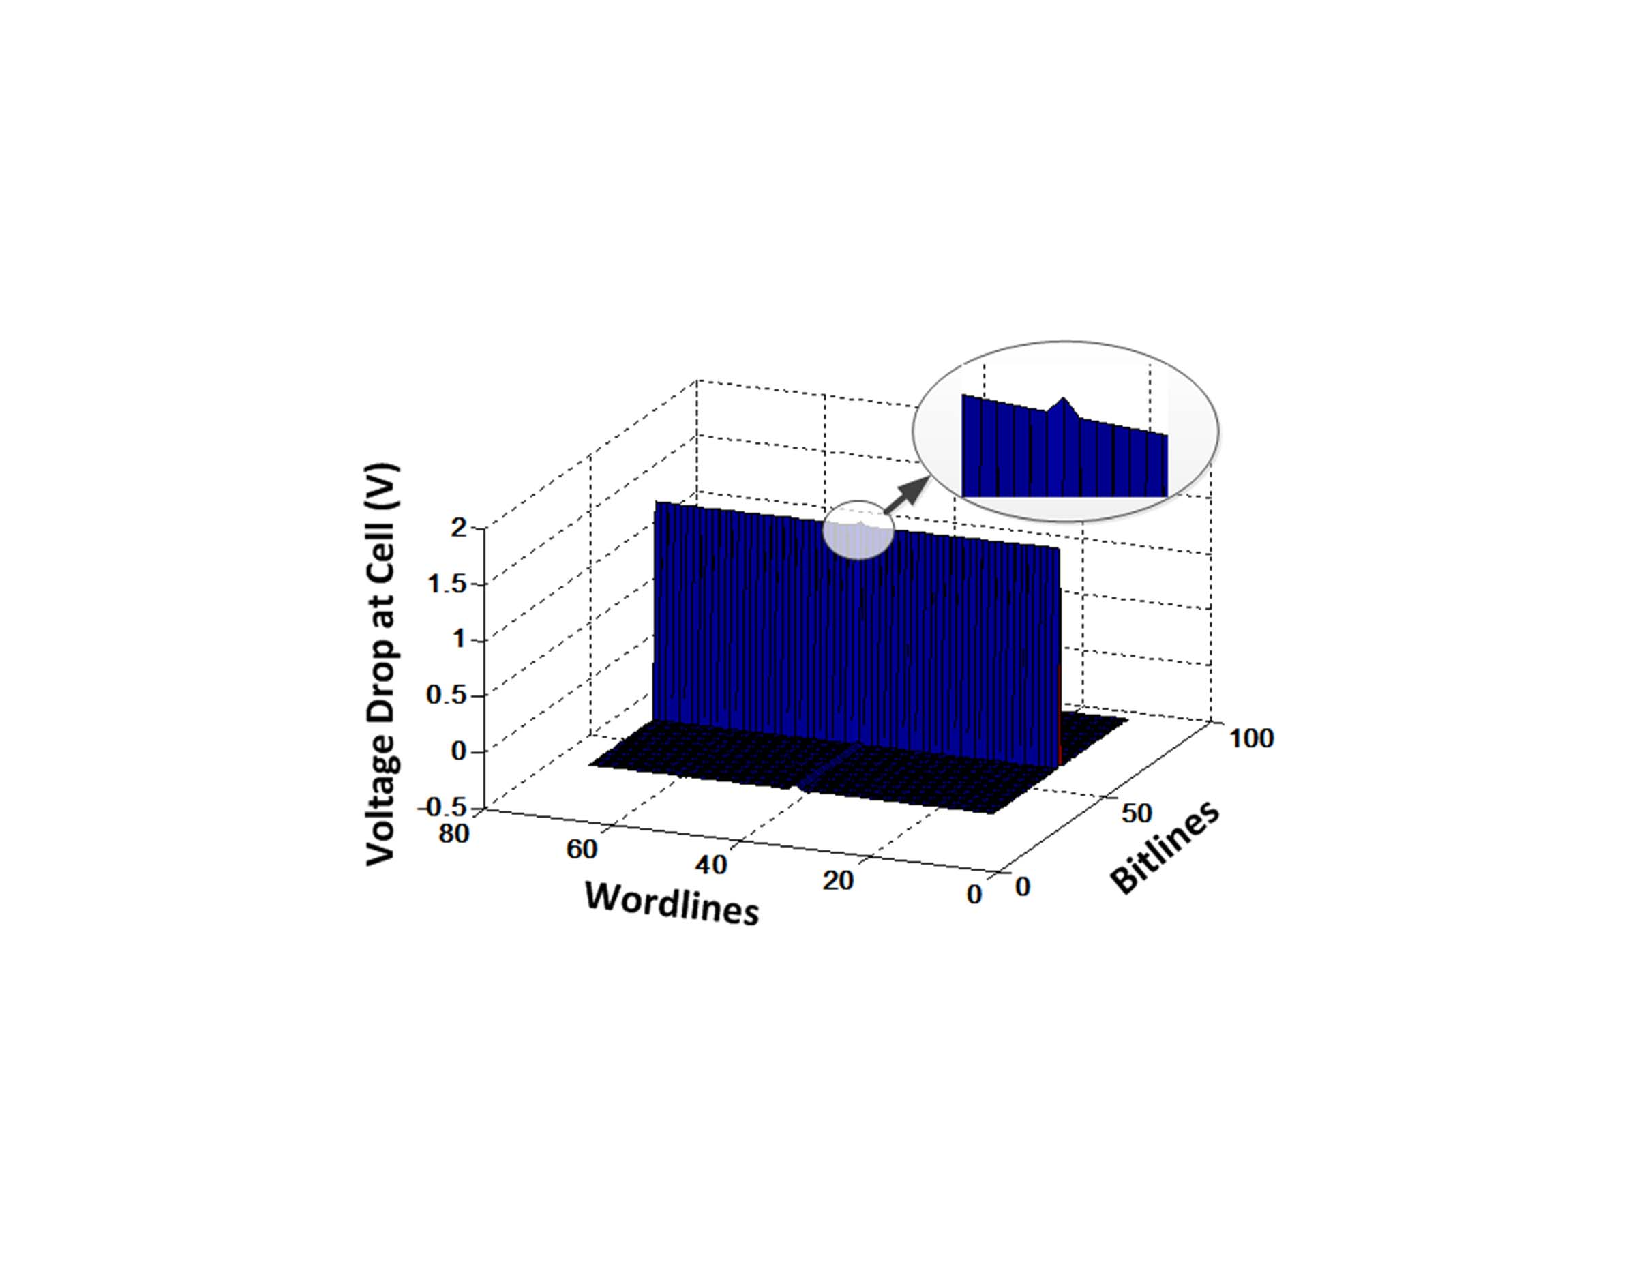
\includegraphics[width=0.4\textwidth]{./figures/FWFB_f.pdf}\\
%  \caption{Write disturbance for FWFB schemes. ( $V_{W32} = 2V$, $V_{B32} = 0V$. $R_{x,32}$ at HRS, others at LRS.) }\label{fig:FWFR}
%\end{figure}
%Considering that the reported On-OFF resistance ratio of
%ReRAM cell is always $>50$ ~\cite{ReRAM_IEDM2010_Ho,ReRAM_IEDM2010_Chien,ReRAM_IEDM2010_Lee_Diode,ReRAM_IEDM2010_Lee_Evidence,ReRAM_ISSCC2011_Sheu,ReRAM_ISSCC2011_Otsuka},
%, the worst case voltage drop at the unselected cell is larger than $98\%$ of the voltage at the selected cell, making it is impossible to build a reliable cross-point structure ReRAM with the FWFB scheme. Therefore, in the following discussion, we only compare the results of FWHB, HWFB and HWHB schemes. For each of these three schemes, we can either write the cells at one wordline at the same time or only write one bit per access and separate the write operation to several arrays. In the
%following discussion, we start from one bit per access write operation,
%then the results of one wordline per access method are discussed.


%as long all of unselected cells in the activated wordline (or all of unselected cells in the activated bitline) are at HRS and other cells are in LRS, the voltage drop at unselected cells are mainly applied at the HRS cells at the wordline (or bitline).
%The worse case scenario for FWFB write disturbance can be defined as: all of unselected cells in the activated wordline (or all of unselected cells in the activated bitline) are at HRS and other cells are in LRS. In this case, the voltage drop at unselected cells are mainly applied at the HRS cells at the wordline (or bitline).

Write failure typically results from the voltage drop at the interconnect
wires along the wordline and bitline. It has been shown that, for
single-bit write operation, the worst case voltage drop occurs when
writing the cell at the cross point of the $M^{th}$ wordline and the
$N^{th}$ bitline with all of the other cells in the array are in
LRS~\cite{crossbar_TED_2010}. In order to avoid write failure and
successfully program the selected ReRAM cell, the driven voltage should be
boosted to a higher level, making sure that the voltage across the cell
exceeds the threshold voltage even at the worst case.
Figure~\ref{fig:worst_v} shows the lower bounds of the driven voltage for
different sizes of cross-point array. The minimum wordline/bitline voltage
increases from 2.01~V for a $32 \times 32$ array to nearly 7~V for a $1024
\times 1024$ cross-point array. However, boosting the driven voltage also
increases the voltage applied at unselected cells. Therefore, a write
disturbance may occur when the voltage applied at an unselected cell
exceeds the threshold voltage for SET or RESET operation. According to our
analysis, the maximum voltage applied at unselect cells is exactly the
same as half of the driven voltage. Thus, only arrays with driven voltage
less than 4V are allowable. Otherwise, the array is unreliable because it
cannot avoid write failure and write disturbance at the same time. The
unreliable array sizes are denoted as red bars in
Figure~\ref{fig:worst_v}. The array size limitation provided by
Figure~\ref{fig:worst_v} is a hard constraint, and all of the following
energy and area trade-offs are bounded by this constraint.

Additionally, the cross-point array can be organized with a different
number of wordlines and bitlines. For example, a 256K bit cross-point
array can be implemented either by a $512 \times 512$ array or by a $64
\times 4096$ array. In the latter case, the voltage drops along the
wordline will be much worse than along the bitline. Figure~\ref{fig:shape}
examines the voltage requirements for different array organizations with
different write schemes. This result shows that from a reliability point
of view, a cross-point array with the same number of wordlines and
bitlines is the best choice. Thus, in the following discuss, we assume the
array has the same number of wordline and bitline. Furthermore, we also
notice that when the array has the same number of wordlines and bitlines,
FWFB, HWFB and FWHB schemes have the same minimum driven voltage.


\begin{figure}%[!hb]
\centering
\hspace{-5pt}
  % Requires \usepackage{graphicx}
  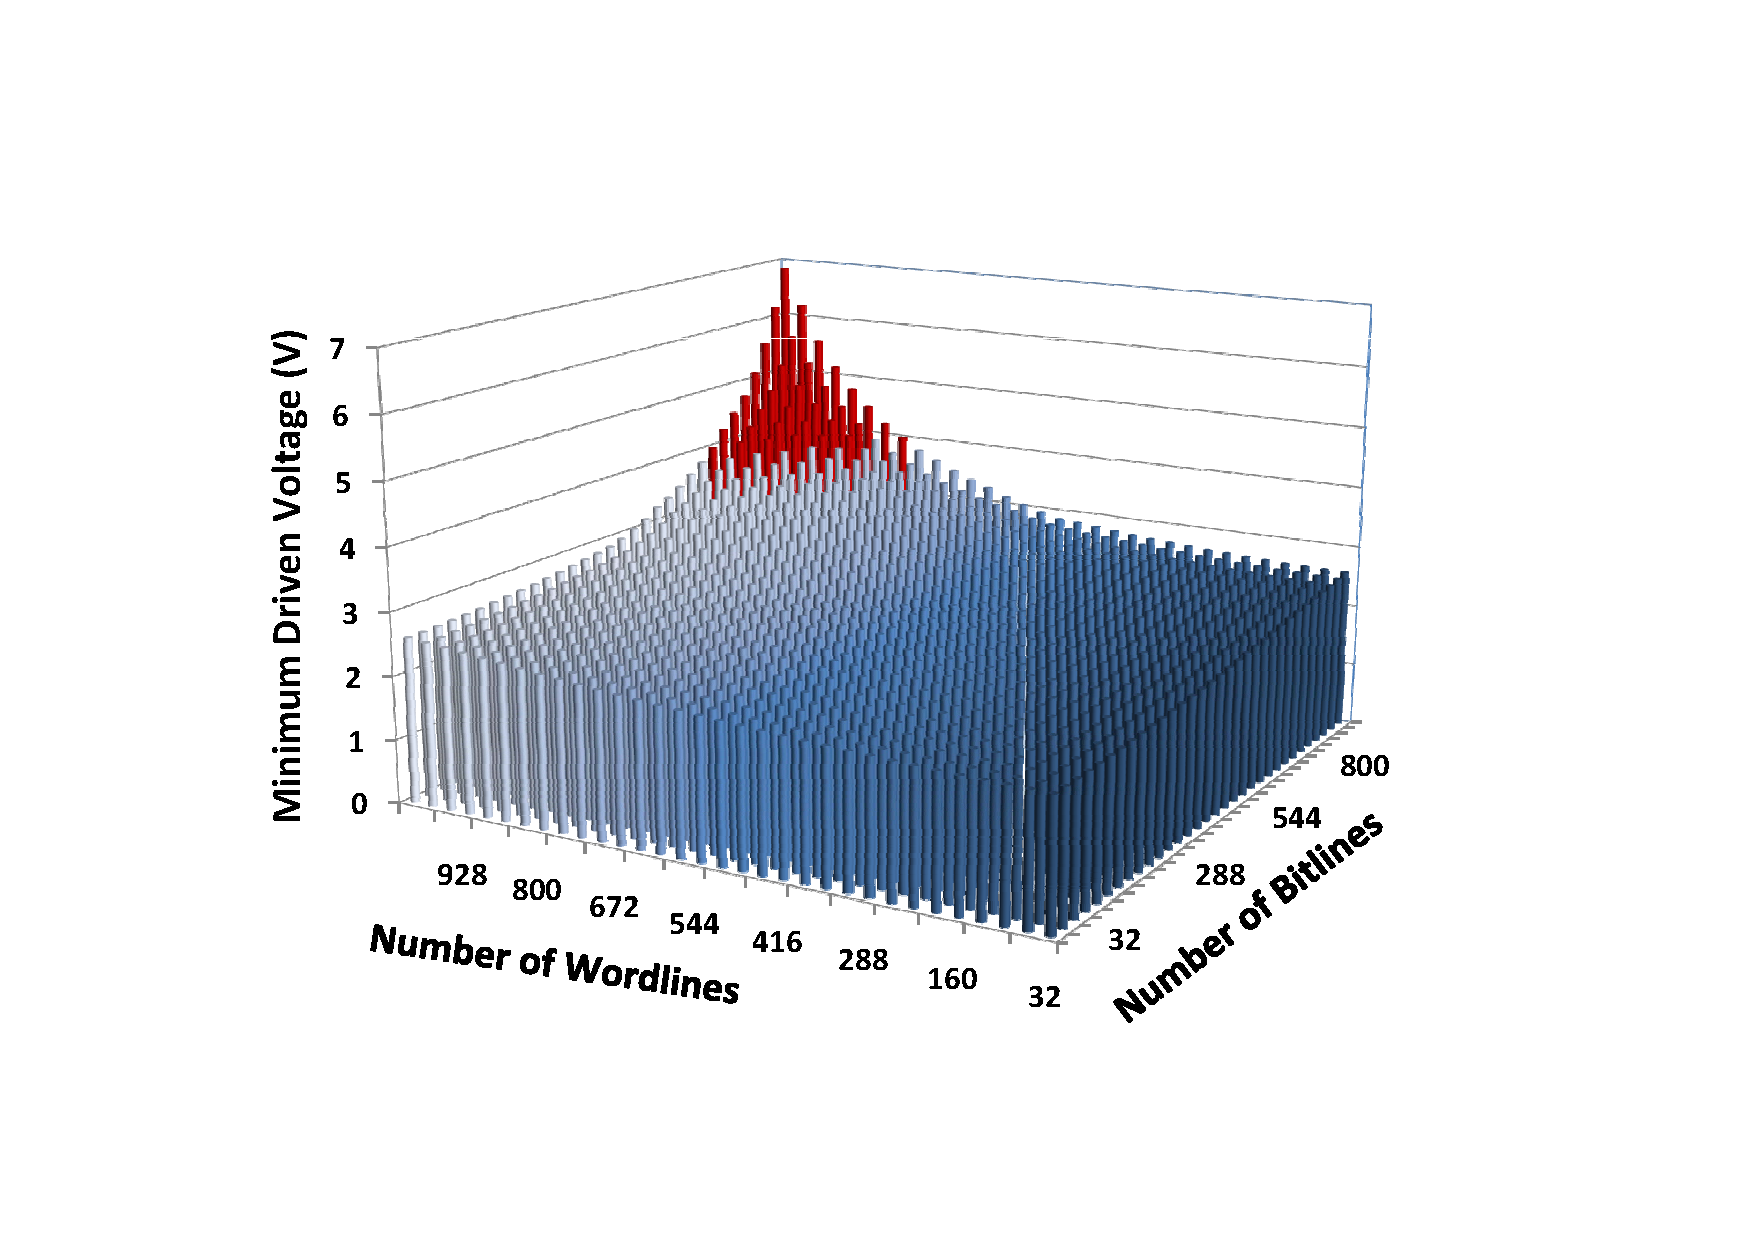
\includegraphics[width=0.4\textwidth]{./figures/worst_v_f1.pdf}\\
  \caption{Required write voltages for different cross-point arrays (threshold voltage = 2V.). }\label{fig:worst_v}
  \vspace{-5pt}
\end{figure}


\begin{figure}%[!t]
\centering
  % Requires \usepackage{graphicx}
  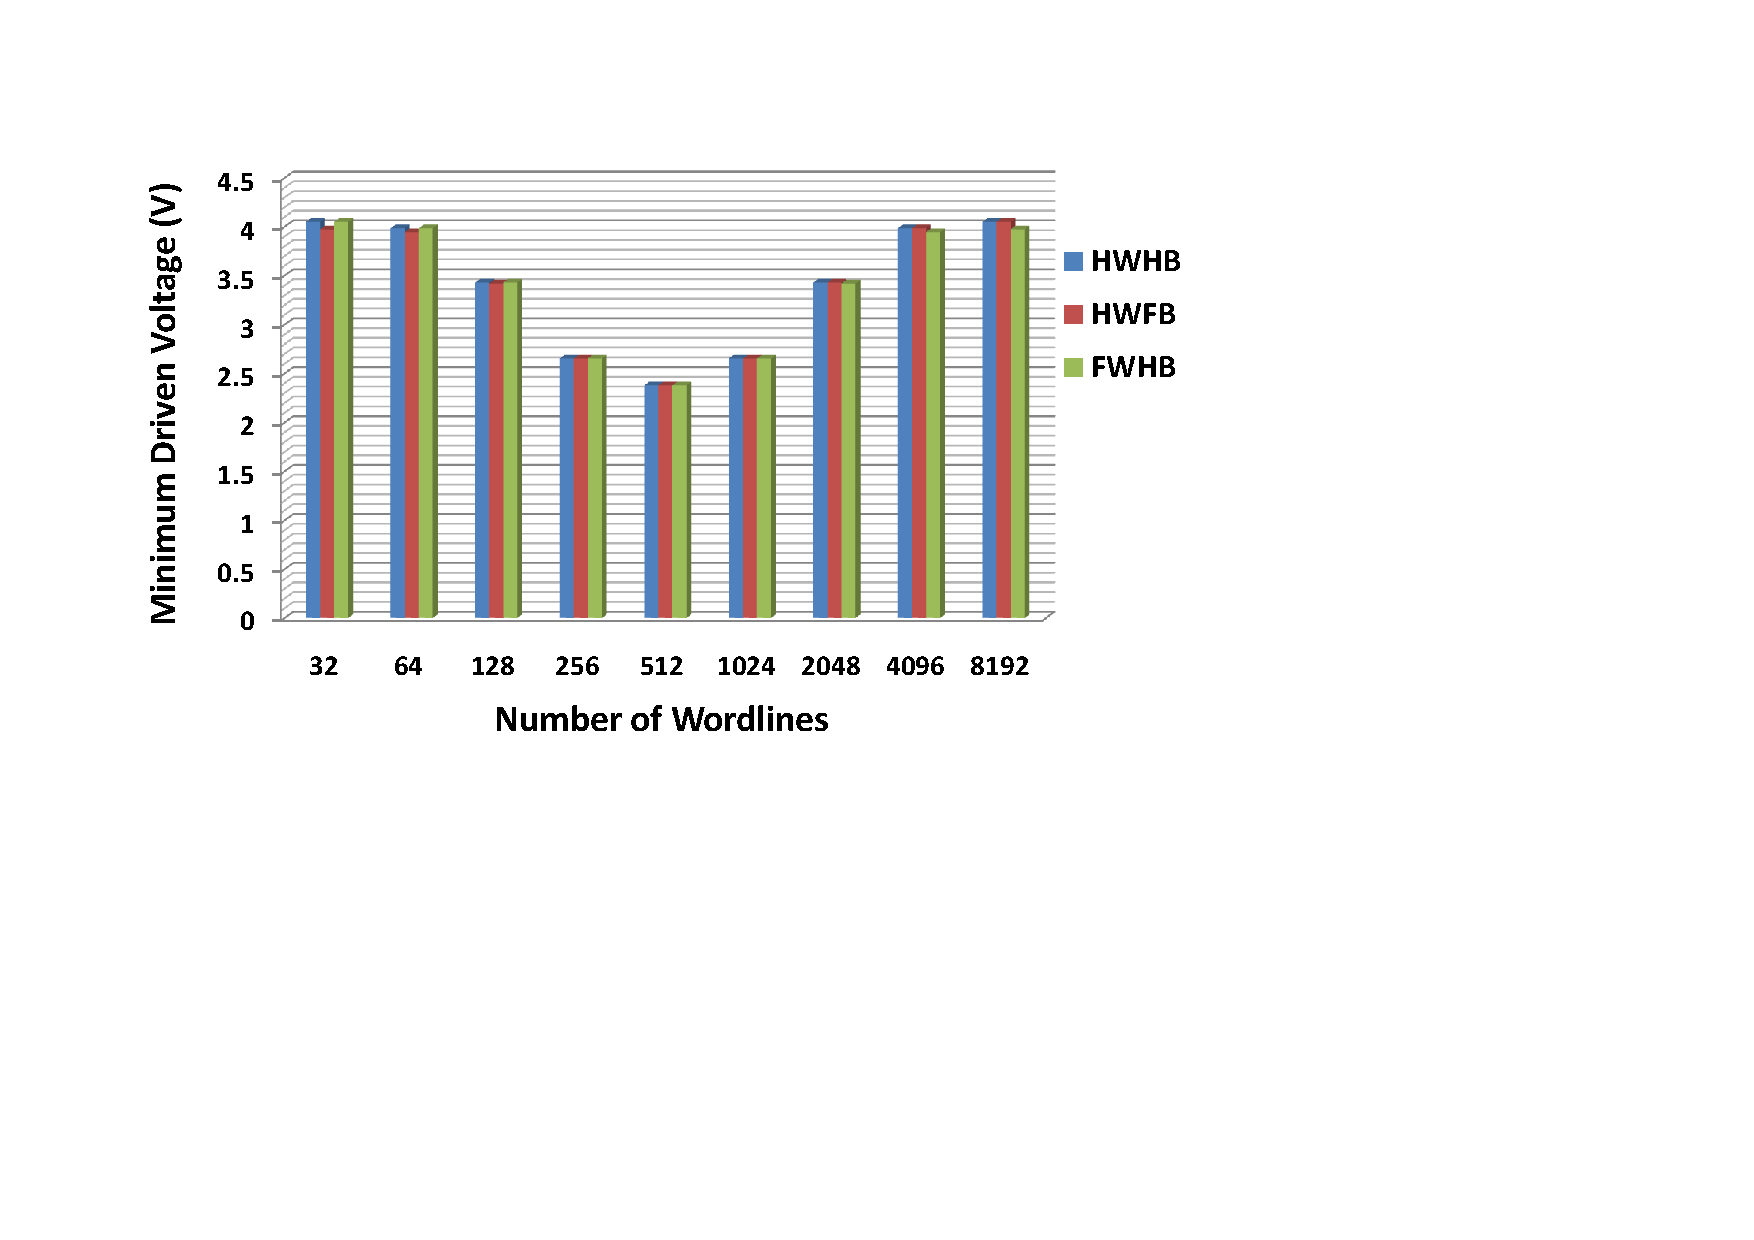
\includegraphics[width=0.4\textwidth]{./figures/shape_f.pdf}\\
  \caption{Required write voltages with different memory shapes (array capacity = 256Kbits, threshold voltage = 2V).}\label{fig:shape}
    \vspace{-15pt}
\end{figure}




%Figure~\ref{fig:half} shows the maximum voltage applied at unselected
%cells with the minimum driven voltage, which is determined in
%Figure~\ref{fig:worst_v}. Since the threshold voltage of the ReRAM cell is
%2V, only array sizes with worst case unselected cell voltage less than 2V
%are allowable. Otherwise, the array is unreliable because it can not avoid
%write failure and write disturbance at the same time. Therefore,
%Figure~\ref{fig:half} provides a hard constraint on array size, and all of
%the following energy and area tradeoffs should be bounded by this
%constraint.

%\begin{figure}%[!t]
%\centering
%  % Requires \usepackage{graphicx}
%  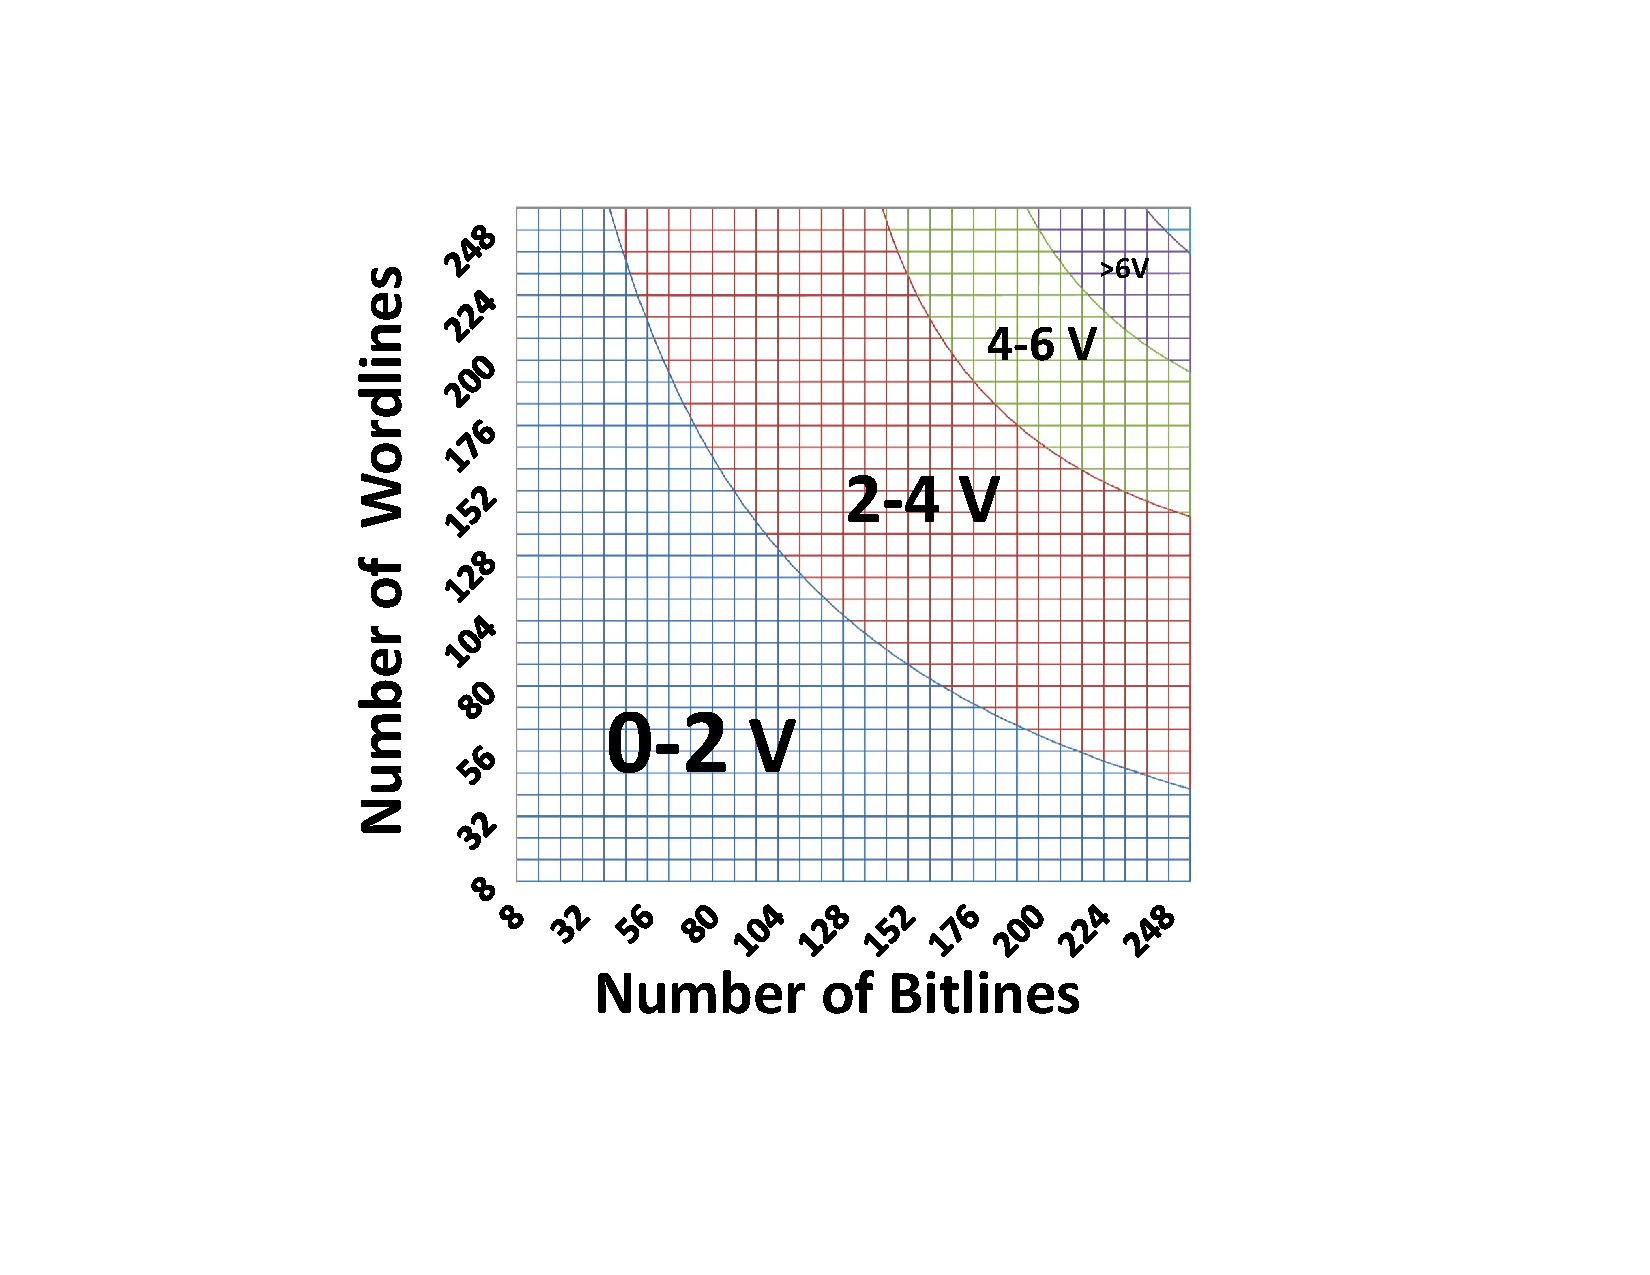
\includegraphics[width=0.28\textwidth]{./figures/Theoretical_bound_f.pdf}\\
%  \caption{The maximum voltage applied at unselected cells with the minimum driven voltage.}\label{fig:half}
%  \vspace{-10pt}
%\end{figure}


\vspace{5pt}\noindent\textbf{Energy Consumption of Write Operations.}
%
%The energy consumption of a write operation for a cross-point array can be calculated as:
%\begin{equation}
%E_{write} = E_{select} + E_{unselect} + E_{halfselect} + E_{line},
%\end{equation}
%where the $E_{select}$ is the energy consumed to change the state of the
%selected cell, the $E_{unselect}$ and $E_{halfselect}$ are the undesired
%energy wasted at the half selected and unselected cells. The energy
%consumed by the interconnect lines are represented by $E_{line}$.
%Figure~\ref{fig:energy} shows the decomposed energy consumption for the
%cross-point array. Note that, the $E_{line}$ and $E_{halfselect}$ take a
%large amount of the total energy consumption. Also, this part of energy
%wasted during the write operation takes greater part of the total energy
%for larger array sizes. For example, the undesired energy consumption for
%writing a $128{\times}128$ array is more than 1000 times larger than the
%$8{\times}8$ array. We also notice that, since the impact of sneak paths
%for floating schemes (FWHB and HWFB) is more serious, the energy consumed
%at unselected cells for floating schemes is larger than the half-biased
%scheme. Due to this reason, the total energy consumptions for FWHB and
%HWFB schemes are at least 10\% larger than that of HWHB scheme.
The energy consumption of a write operation includes: the energy consumed
to change the state of the selected cell, the undesired energy wasted at
the half selected cells and unselected cells, and the energy consumed by
the interconnect lines. Intuitively, the impact of sneak paths for
floating schemes (FWHB and HWFB) is more serious, the energy consumed at
unselected cells for floating schemes should be larger than the HWHB
scheme. However, our simulation results show that compared to the total
energy consumption, the energy consumed by unselected cells are
negligible. Therefore, the total energy consumptions for FWHB and HWFB
schemes are almost the same as that of HWHB scheme. In addition, as
mentioned, the voltage drop results for these schemes are also similar, in
the following discussion, we only show the simulation results of HWHB
scheme. The results for the other two schemes have the same trend as that
of HWHB scheme.

Figure~\ref{fig:energy}(a) shows the decomposed energy consumption for
single-bit write operation. Obviously, the undesired energy consumed by
half-selected cells takes a great part of the total energy consumption.
Besides, with the increase of array size, the energy dissipated at
interconnect lines also becomes significant. Also, this part of the energy
wasted during the write operation is a greater part of the total energy
for larger array sizes. For example, the undesired energy consumption for
writing a $512{\times}512$ array is more than 15 times larger than that of
a $32{\times}32$ array. For multi-bit write operation, we evaluate the
energy consumption of write operations that program the entire wordline at
one time. In order to fairly compare the energy consumption, we compare
the energy-per-bit instead of the total energy. For example, in order to
write a wordline with size of 512 bits, the energy-per-bit can be
calculated as: $E_{ave}=E_{total}/512$. Figure~\ref{fig:energy}(b) shows
the energy-per-bit of the multi-bit write operation. Compared with the
single-bit write operation, we conclude that for large cross-point array
sizes, the multi-bit write operation is much more energy efficient. This
is because the energy wasted at the unselected and half-selected cells are
amortized by multiple bits and the average energy for one bit is therefore
reduced.

\begin{figure}%[!t]
\centering
  % Requires \usepackage{graphicx}
  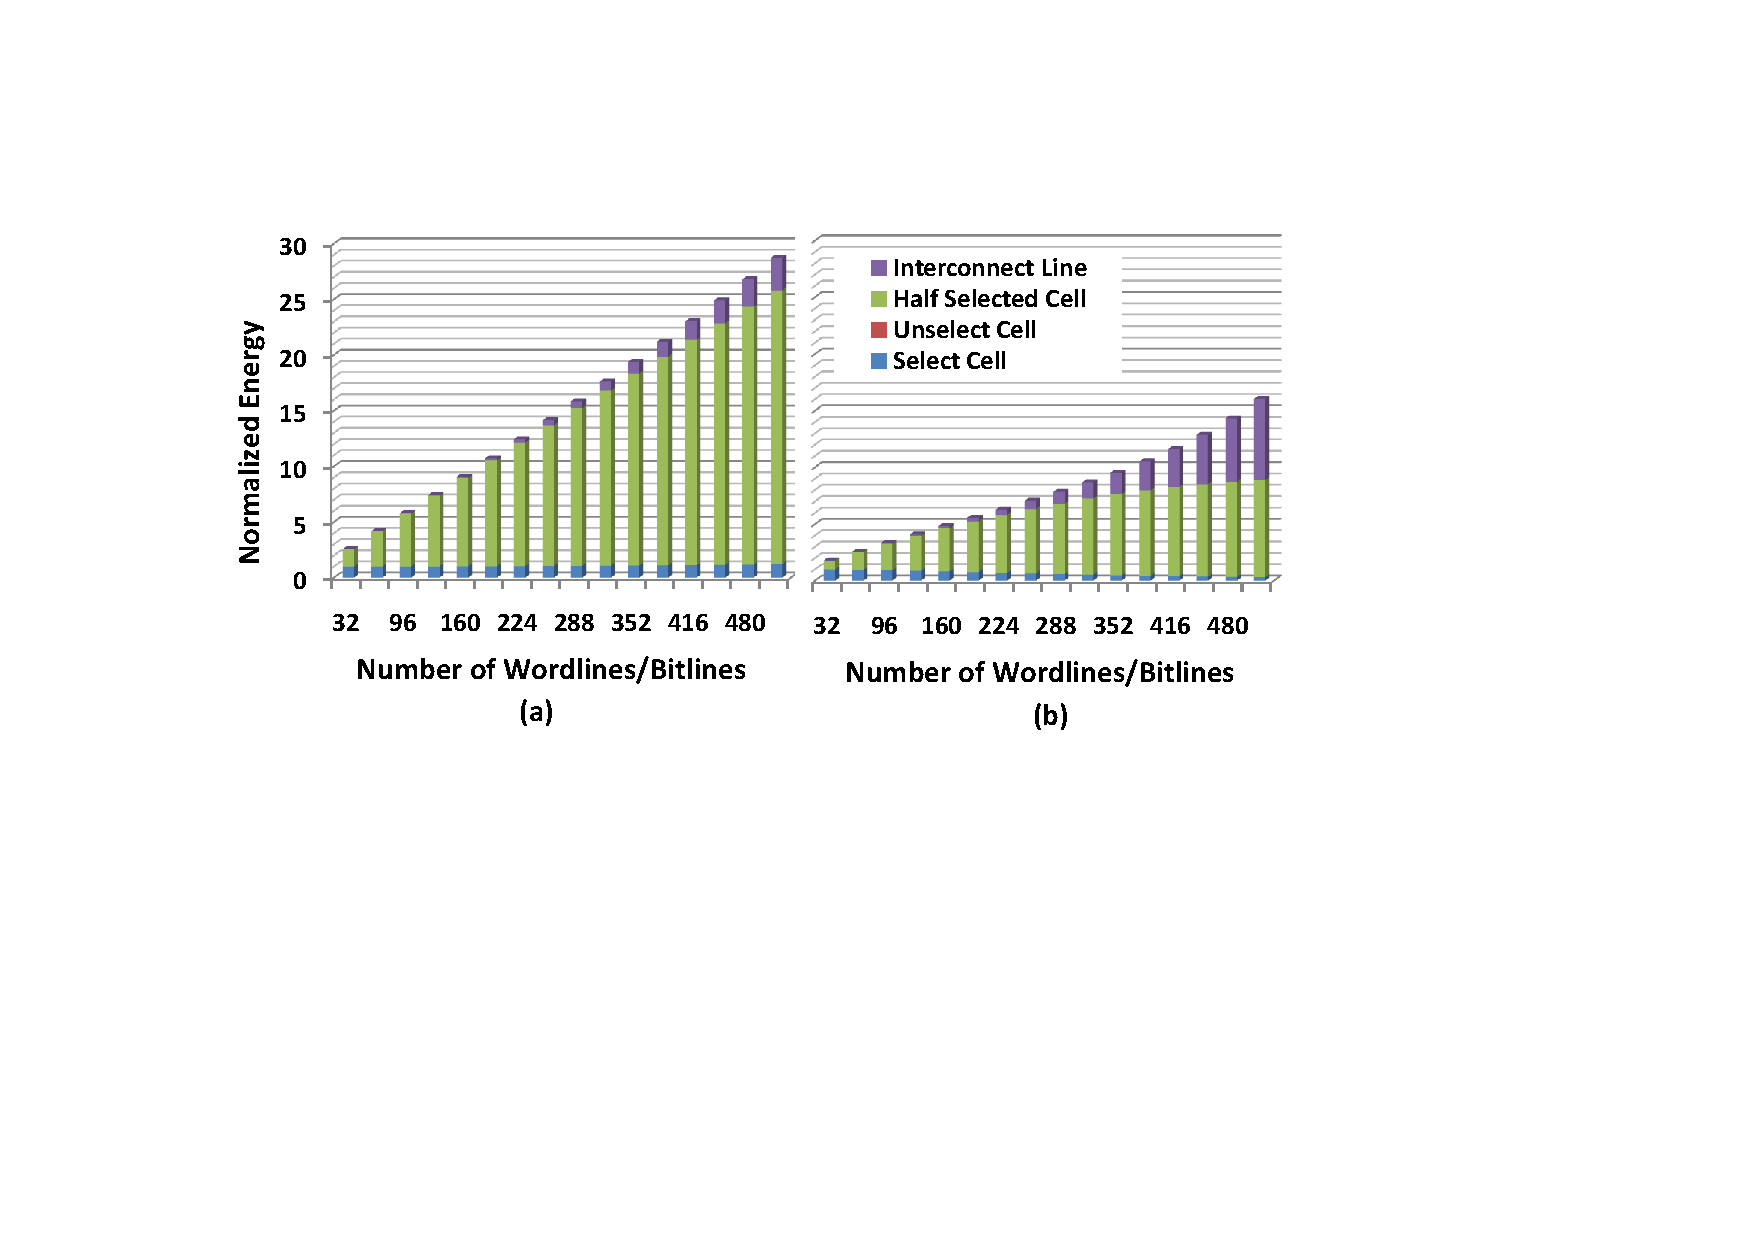
\includegraphics[width=0.5\textwidth]{./figures/energy_f_tall2.pdf}\\
  \caption{The normalized energy consumption with different array size. (a) Single-bit writing. (b) Multi-bit writing.}\label{fig:energy}
    \vspace{-10pt}
\end{figure}

\vspace{5pt}\noindent\textbf{Write Current and Area Overhead of Write Operations.}
%\vspace{6pt}
%
The write operation for a $M \times N$ array requires $M$ wordline voltage
drivers and $N$ bitline multiplexors. The drivers and multiplexors should
be sized such that they can provide the worst-case current of wordline
current and bitline current. The transistor sizing of the wordline/bitline
circuitry is achieved using HSPICE simulations. We further calculate the
area overhead for the drivers and multiplexors by referring to the CACTI
area model. Figure~\ref{fig:drive_i}(a) shows the maximum write current
with different ReRAM array sizes. Not surprisingly, the current
requirement increases as the array size increases.
Figure~\ref{fig:area_i}(a) illustrates the area overhead for the wordline
and bitline circuitry. This show that drivers and multiplexors occupy a
smaller area than the cross-point array. Only in this case can voltage
drivers and multiplexors be implemented beneath the array, resulting an
ideal cell size of $4F^2$.

Although multi-bit write operation has the advantage of lower energy
consumption, the maximum current requirement for each wordline also
increases. As demonstrated in Figure~\ref{fig:drive_i}(b), although the
maximum driven current for each bitline is almost the same as when writing
one bit, the driving current requirement for each wordline in a multi-bit
write scheme is $>10$ times larger than that of a single-bit write scheme.
Since the area of the voltage driver increases proportionally with its
driving current, the area overhead for multi-bit writing is much larger
than that of single-bit writing. As shown in Figure~\ref{fig:area_i}(b),
the peripheral circuitry area is much larger than that of the array. In
this case, the total area of the memory array is dominated by the
peripheral circuitry rather than the cells. In addition to the extra area
overhead, writing multiple bits at one time also worsens the voltage drop
along the wordline. As shown in Figure~\ref{fig:reliable_region}, in order
to write an entire wordline when writing, the maximum reliable array size
reduces from $800 \times 800$ to $352 \times 352$. This is because the
current passing through the interconnect wires in the multi-bit write
scheme is much larger than that of the single-bit write scheme, causing
more severe voltage drops on the wire resistance.

Therefore, we conclude that although the multi-bit write operation is more
energy efficient, from the standpoint of reliability and area overhead,
single-bit write operation is preferred.
%\begin{figure}%[!t]
%\centering
%  % Requires \usepackage{graphicx}
%  \includegraphics[width=0.4\textwidth]{./figures/w_current2.pdf}\\
%  \caption{The }\label{fig:w_current}
%\end{figure}
\begin{figure}%[!t]
\centering
  % Requires \usepackage{graphicx}
  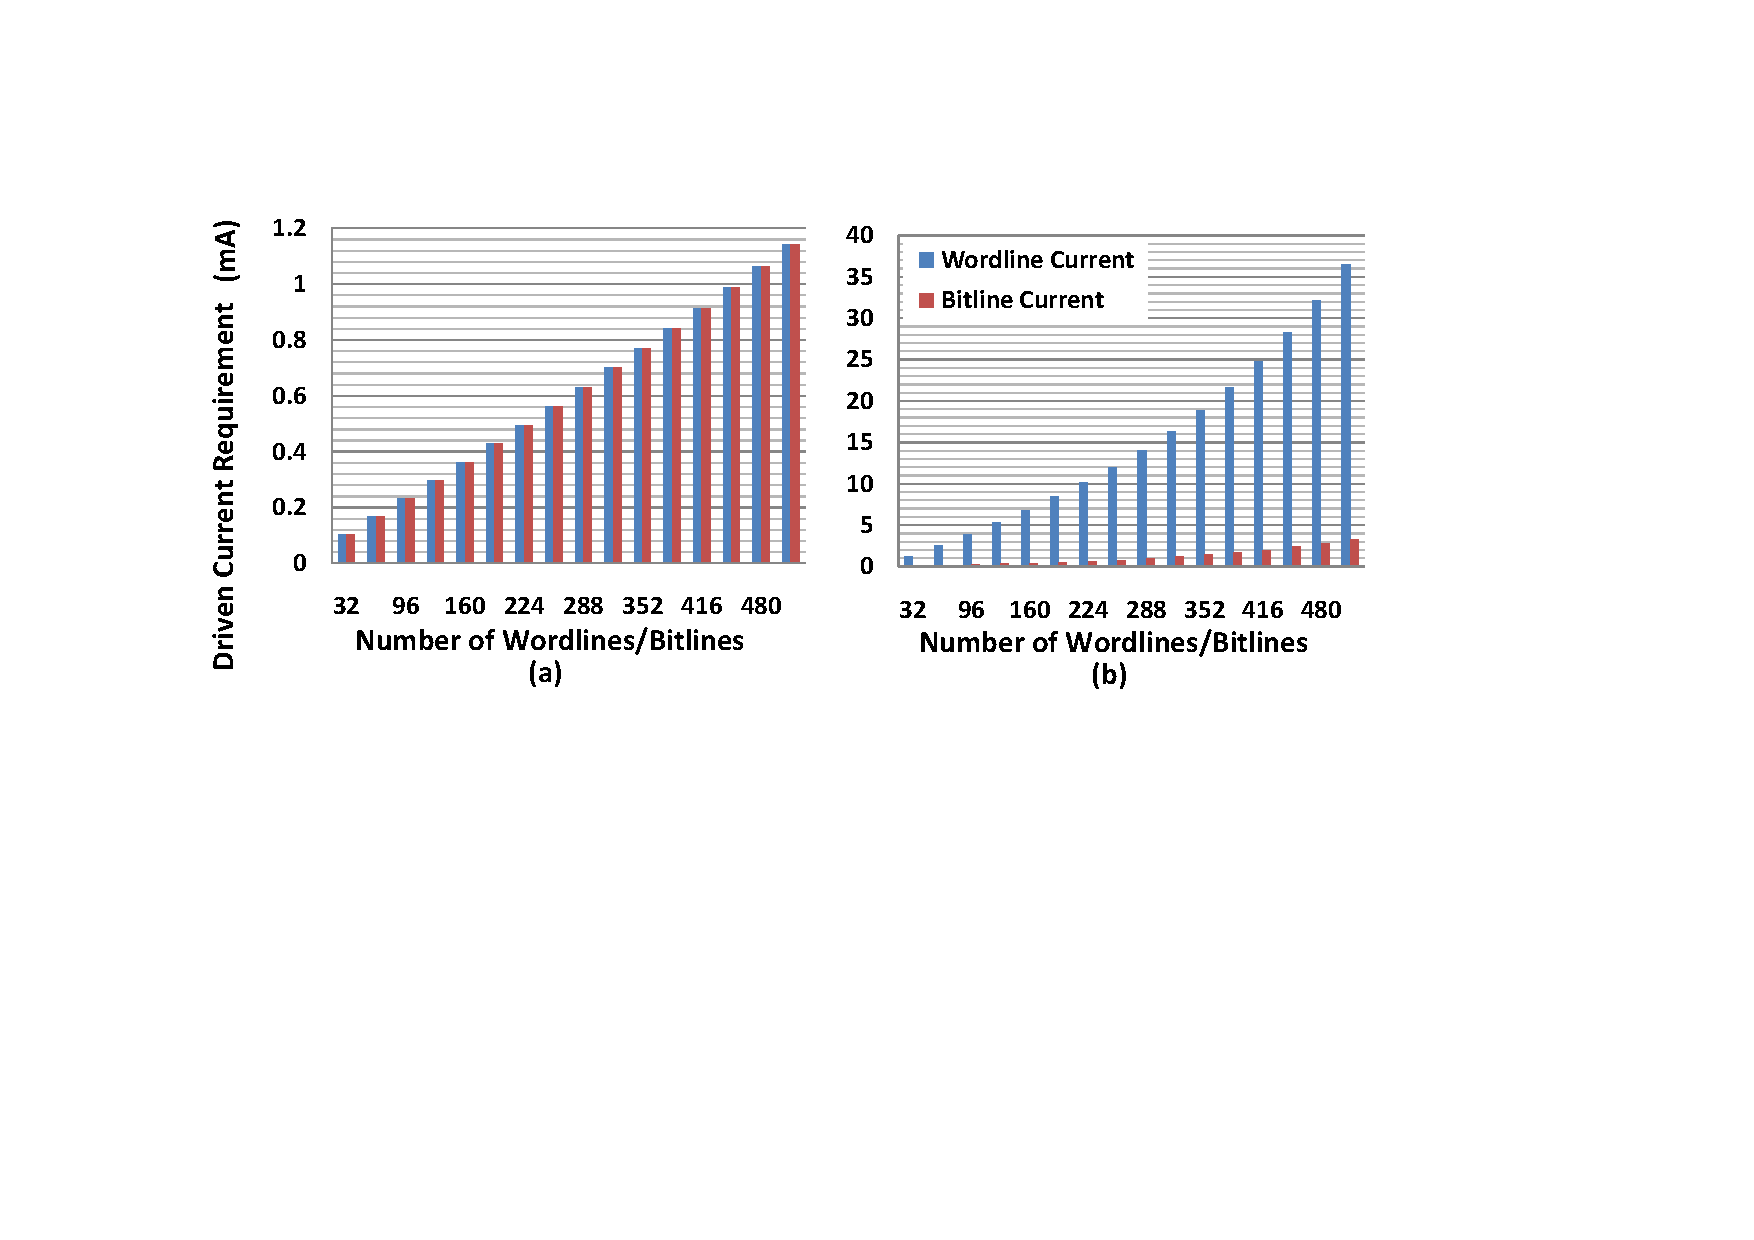
\includegraphics[width=0.5\textwidth]{./figures/drive_i_f.pdf}\\
  \caption{The requirements for wordline and bitline driven currents. (a) One bit per write. (b) One wordline per write.}\label{fig:drive_i}
\end{figure}



\begin{figure}%[!t]
\centering
  % Requires \usepackage{graphicx}
  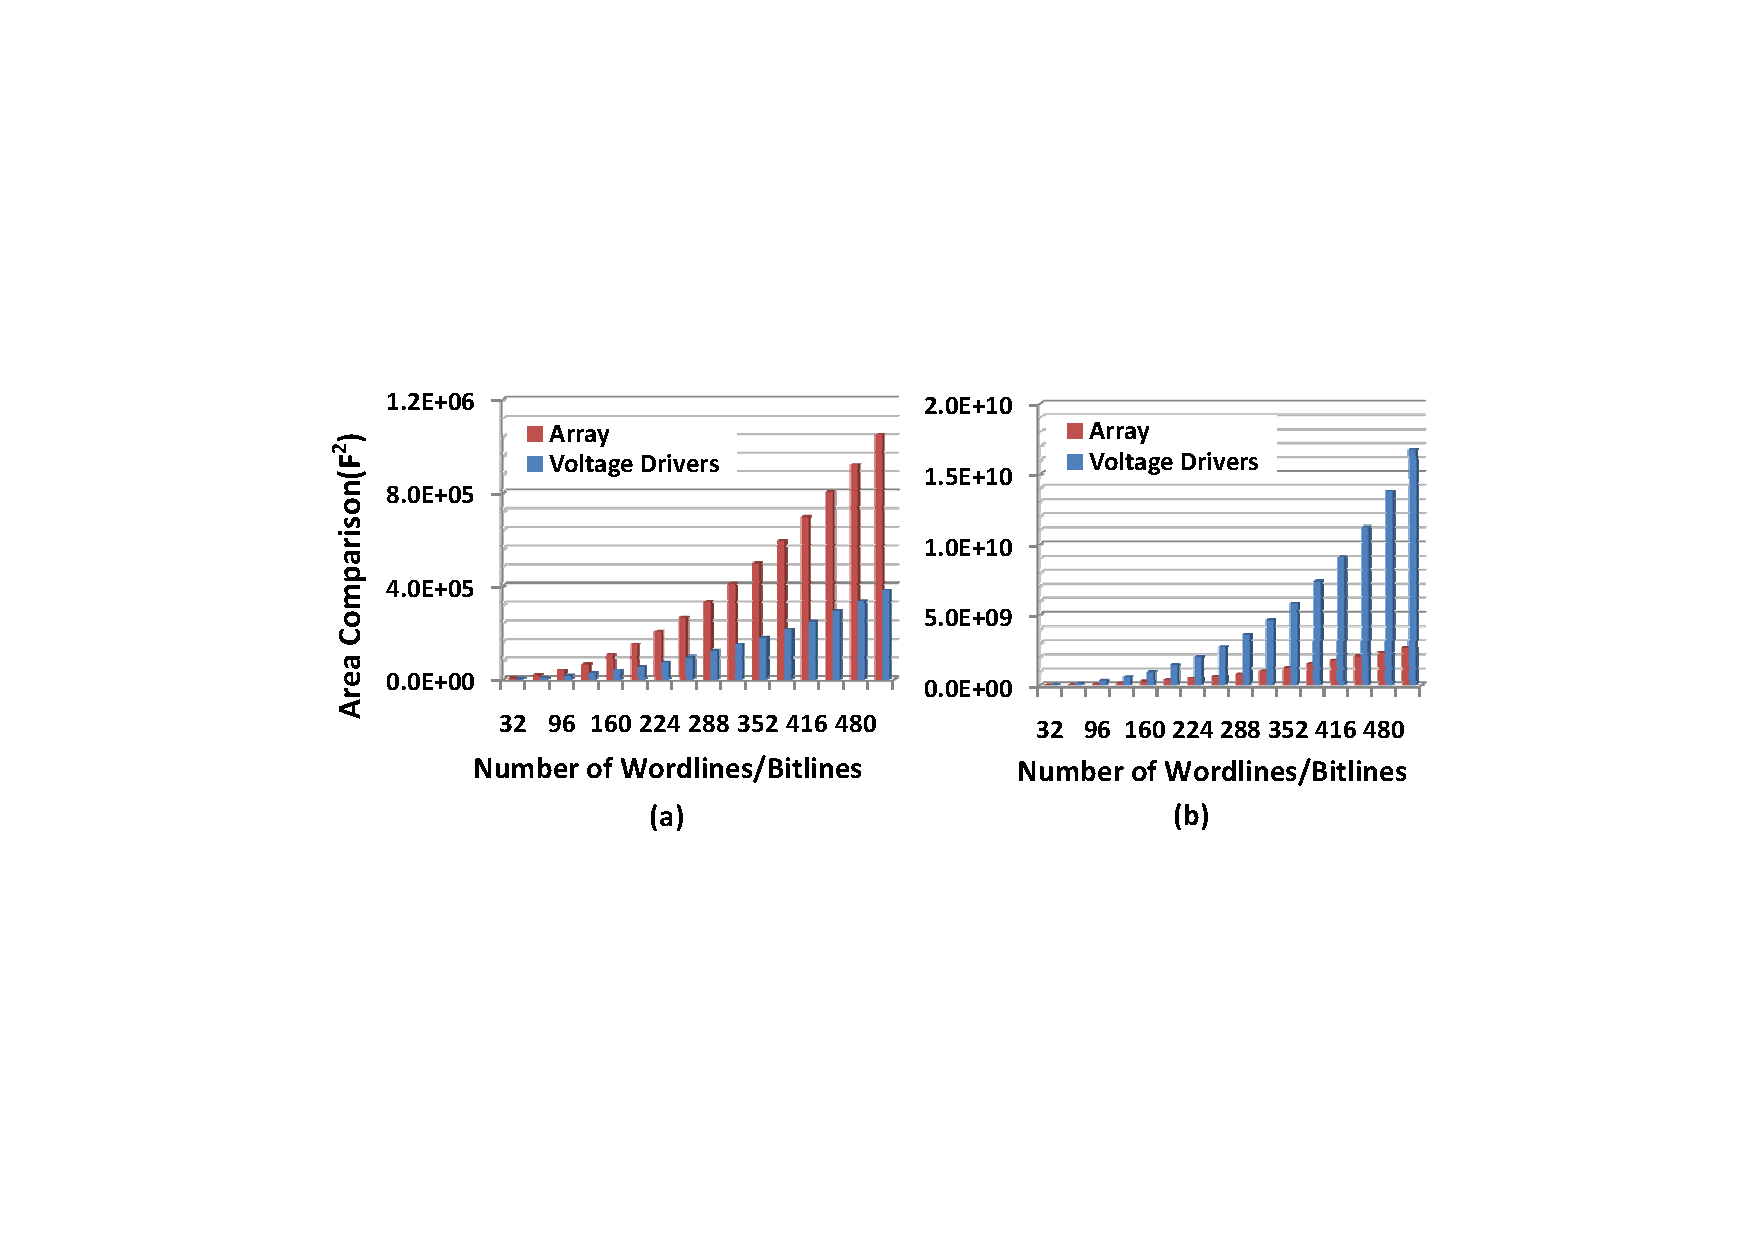
\includegraphics[width=0.5\textwidth]{./figures/area_comp_f1.pdf}\\
  \caption{Area overhead comparison. (a) One bit per write. (b) One wordline per write.}\label{fig:area_i}
\vspace{-10pt}
\end{figure}

%\vspace{5pt}\noindent\textbf{Discussion on Multi-Bits Write Operation.} %\vspace{2pt}
%
%So far, we have only discussed the write operation with one bit per
%access. In this section, we compare the difference between single-bit per
%access and multi-bit per access write operations.
%
%First of all, we evaluate the energy consumption of write operations that
%program the entire wordline at one time. In order to fairly compare the
%energy consumption, we compare the energy-per-bit instead of the total
%energy. For example, in order to write a wordline with size of 512 bits,
%the energy-per-bit can be calculated as: $E_{ave}=E_{total}/512$.

%Figure~\ref{fig:energy}(b) shows the energy-per-bit of the multi-bit write
%operation. Compared with the single-bit write operation as shown in
%Figure~\ref{fig:energy}(a), we conclude that for large cross point array
%sizes, the multi-bit write operation is much more energy efficient. This
%is because the energy wasted at the unselected and half-selected cells are
%amortized by multiple bits and the average energy for one bit is therefore
%reduced.

%%However, although multi-bit write operation has the advantage of lower
%%energy consumption, the maximum current requirement for each wordline also
%%increases. As demonstrated in Figure~\ref{fig:drive_i}(b), although the
%%maximum driven current for each bitline is almost the same as when writing
%%one bit, the driving current requirement for each wordline in a multi-bit
%%write scheme is $>10$ times larger than that of a single-bit write scheme.
%%Since the area of the voltage driver increases proportionally with its
%%driving current, the area overhead for multi-bit writing is much larger
%%than that of single-bit writing. As shown in Figure~\ref{fig:area_i}(b),
%%the peripheral circuitry area is much larger than that of the array. In
%%this case, the total area of the memory array is dominated by the
%%peripheral circuitry rather than the cells.
%%%\begin{figure}%[!t]
%%%\centering
%%%  % Requires \usepackage{graphicx}
%%%  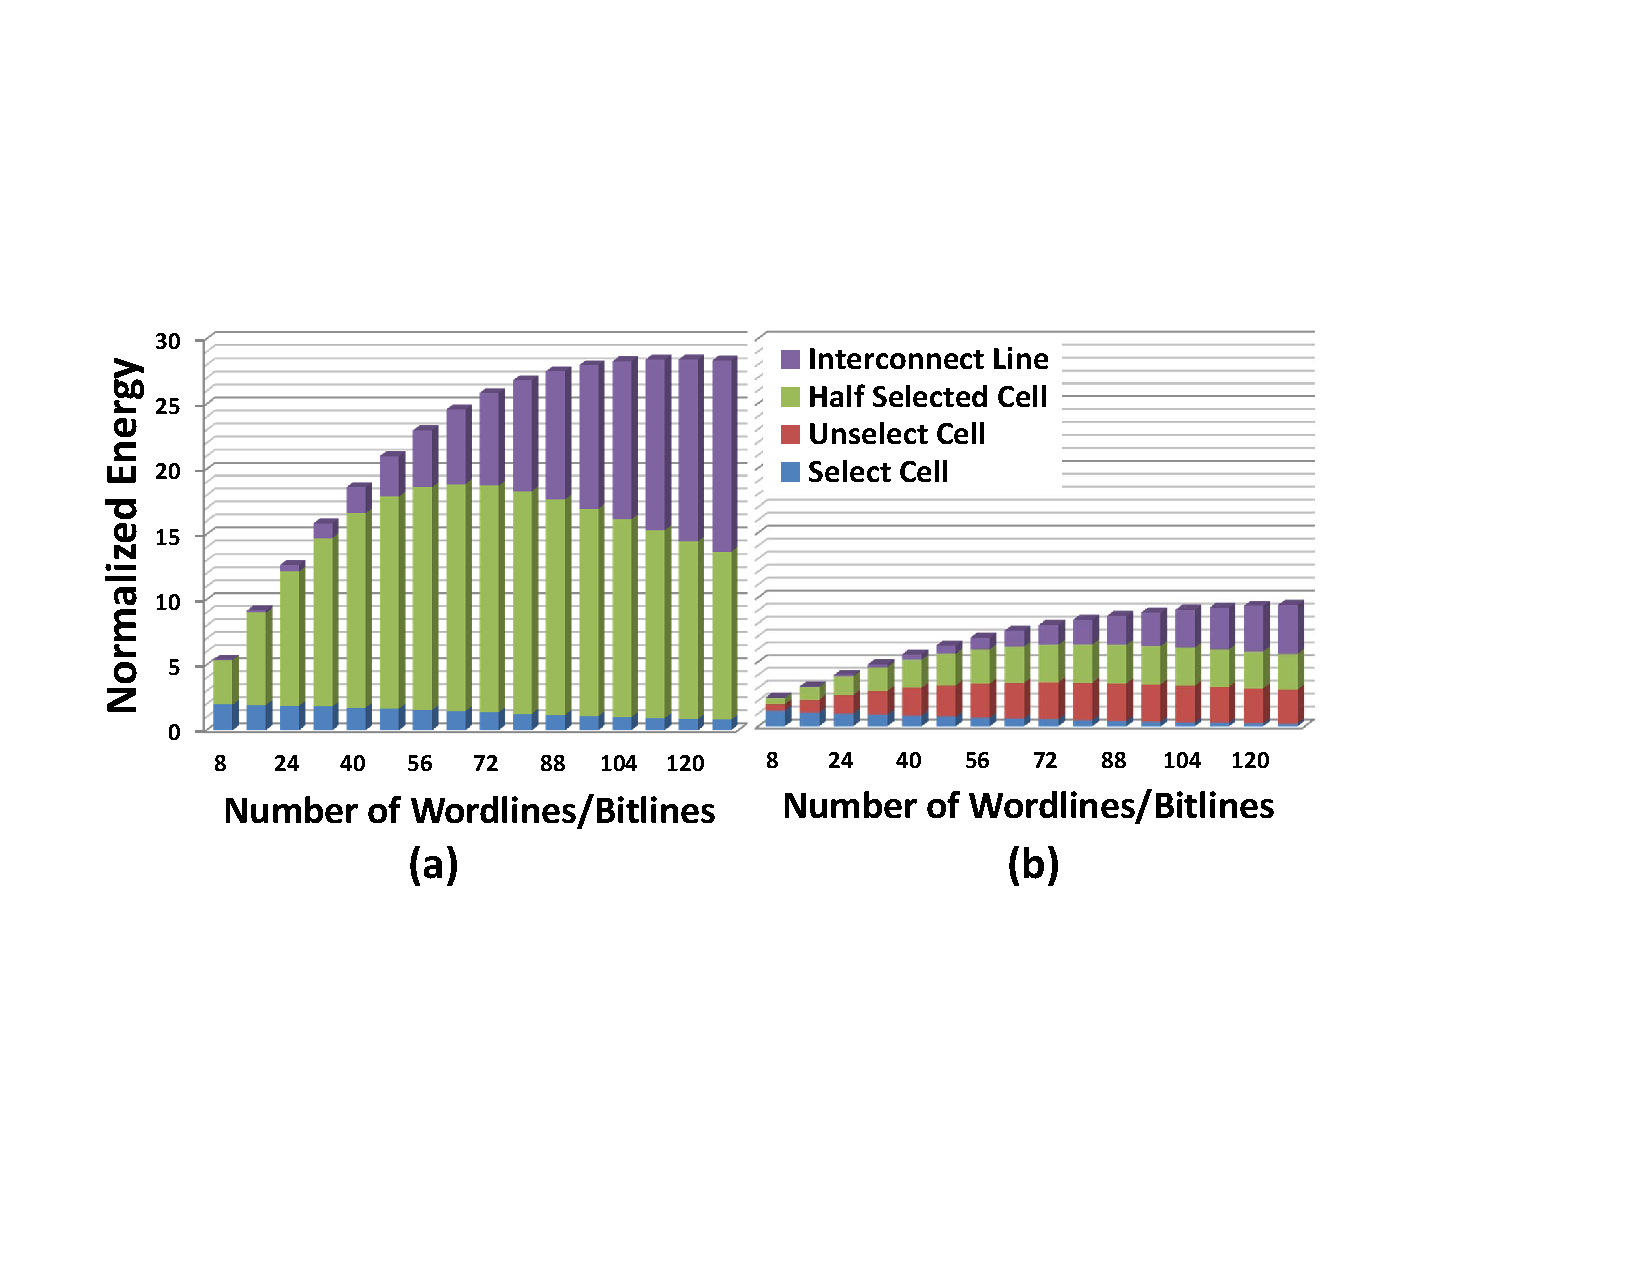
\includegraphics[width=0.5\textwidth]{./figures/multi_energy_f.pdf}\\
%%%  \caption{The normalized energy consumption per bit for multi-bits write operation. (a): HWHB and  FWHB schemes; (b): HWFB scheme. }\label{fig:multi_energy}
%%%    \vspace{-10pt}
%%%\end{figure}
%%In addition to the extra area overhead, writing multiple bits at one time
%%also worsens the voltage drop along the wordline. As shown in
%%Figure~\ref{fig:reliable_region}, in order to write an entire wordline
%%when writing, the maximum reliable array size reduces from $800 \times
%%800$ to $352 \times 352$. This is because the current passing through the
%%interconnect wires in the multi-bit write scheme is much larger than that
%%of the single-bit write scheme, causing more severe voltage drops on the
%%wire resistance.
%%
%%Therefore, we conclude that although the multi-bit write operation is more
%%energy efficient, from the standpoint of reliability and area overhead,
%%single-bit write operation is preferred.


%Figure~9(b) shows that for a $512\times 512$ cross-point array, the worst-case voltage drop increases and eventually become unreliable as we increase the number of bits per write operation. The maximum of bits that can be accessed simultaneously while maintaining reliable write operation is about 130.

%Therefore, as shown in Figure~\ref{fig:reliable_region},
%Therefore the simulation results show that the reliable size of the
%cross-point array will be further reduced. The maximum array size reduces
%from $116{\times}116$ to $100{\times}100$ for HWFB and HWFB schemes.
%For the energy consumption point of view, the one wordline write operation is more efficient.
%\begin{figure}%[!t]
%\centering\label{fig:multiV}
%  % Requires \usepackage{graphicx}
%  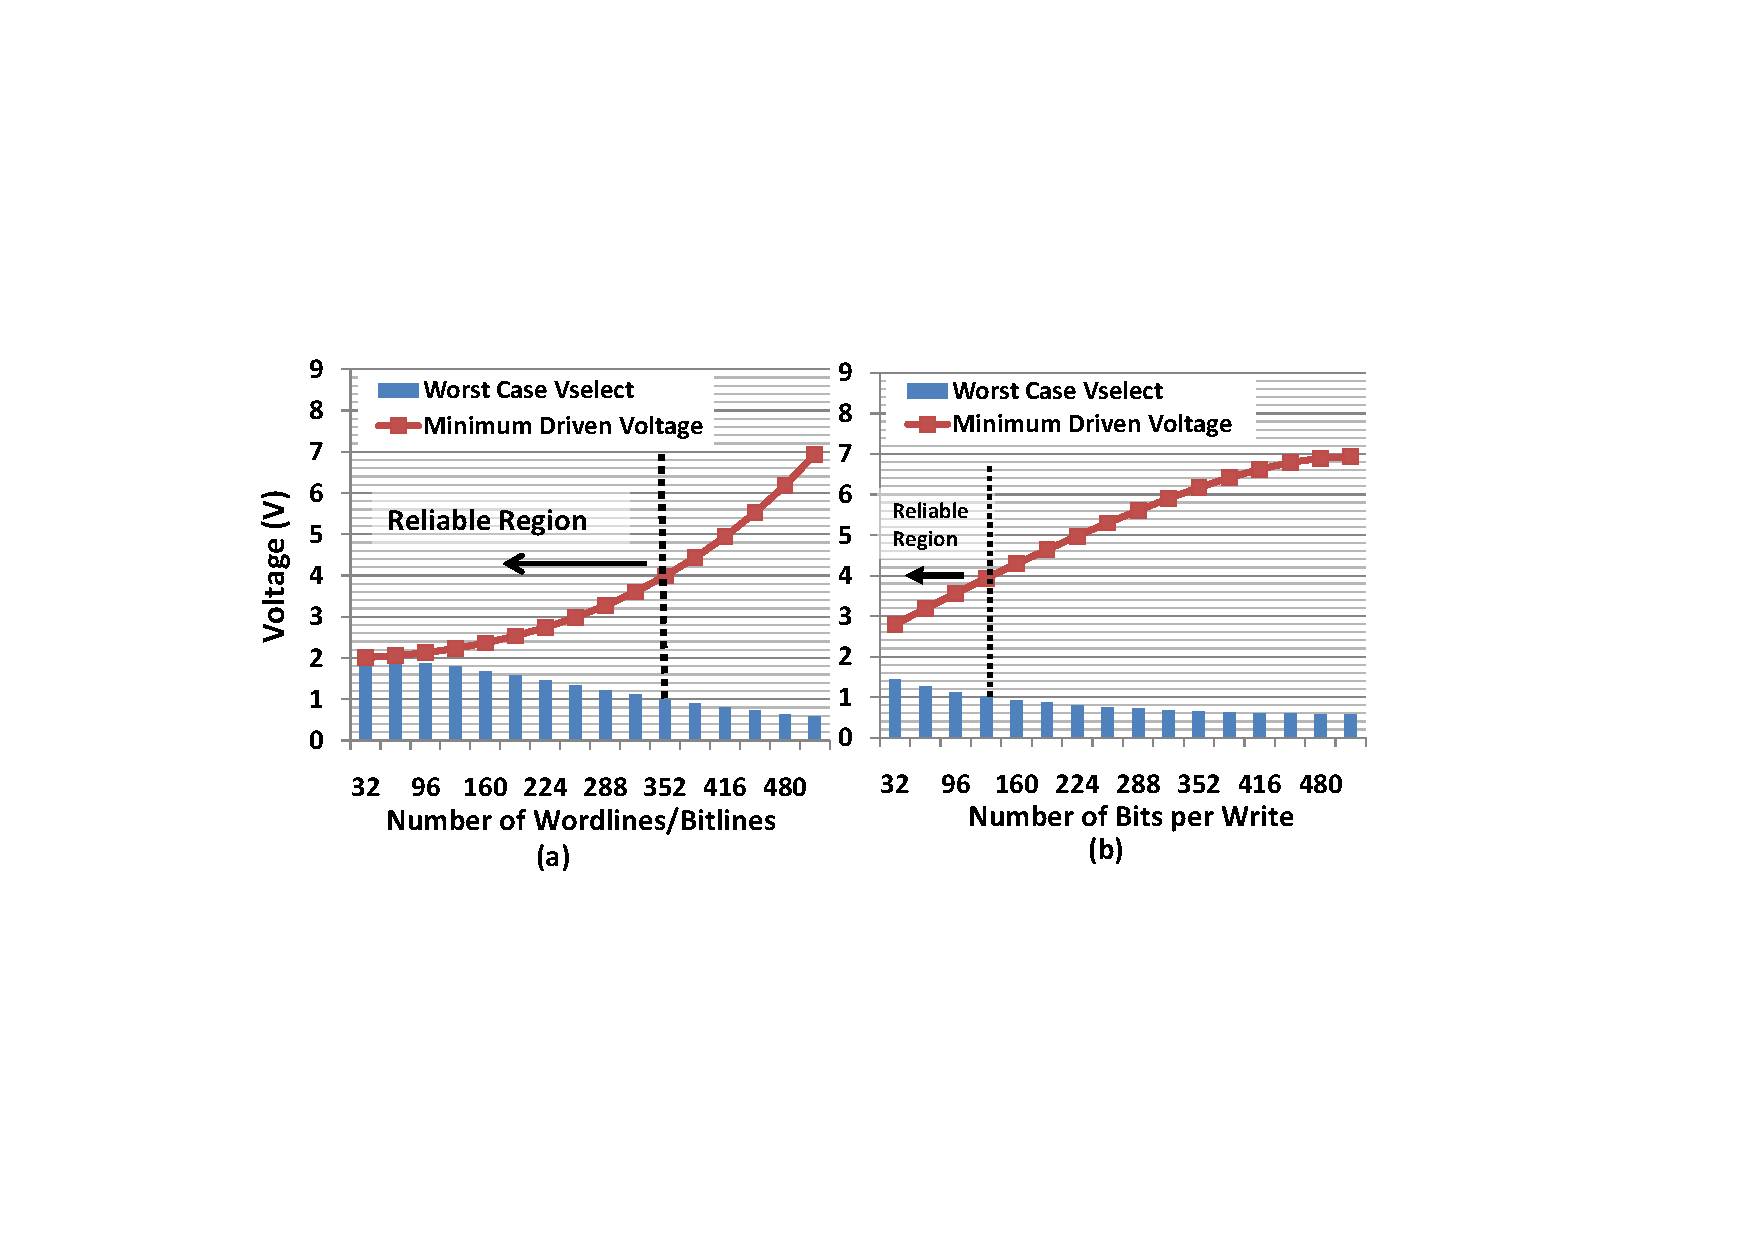
\includegraphics[width=0.5\textwidth]{./figures/multi_V.pdf}\\
%  \caption{Worst case voltage and write voltage requirements for multi-bit writing. (a) Writing all the bits in a wordline at the same time (x-axis denote the different array sizes). (b) Writing various bits per operation in a 512$\times$512 array.}\label{fig:reliable_region}
%    \vspace{-10pt}
%\end{figure}

\begin{figure}%[!t]
\centering\label{fig:multiV}
  % Requires \usepackage{graphicx}
  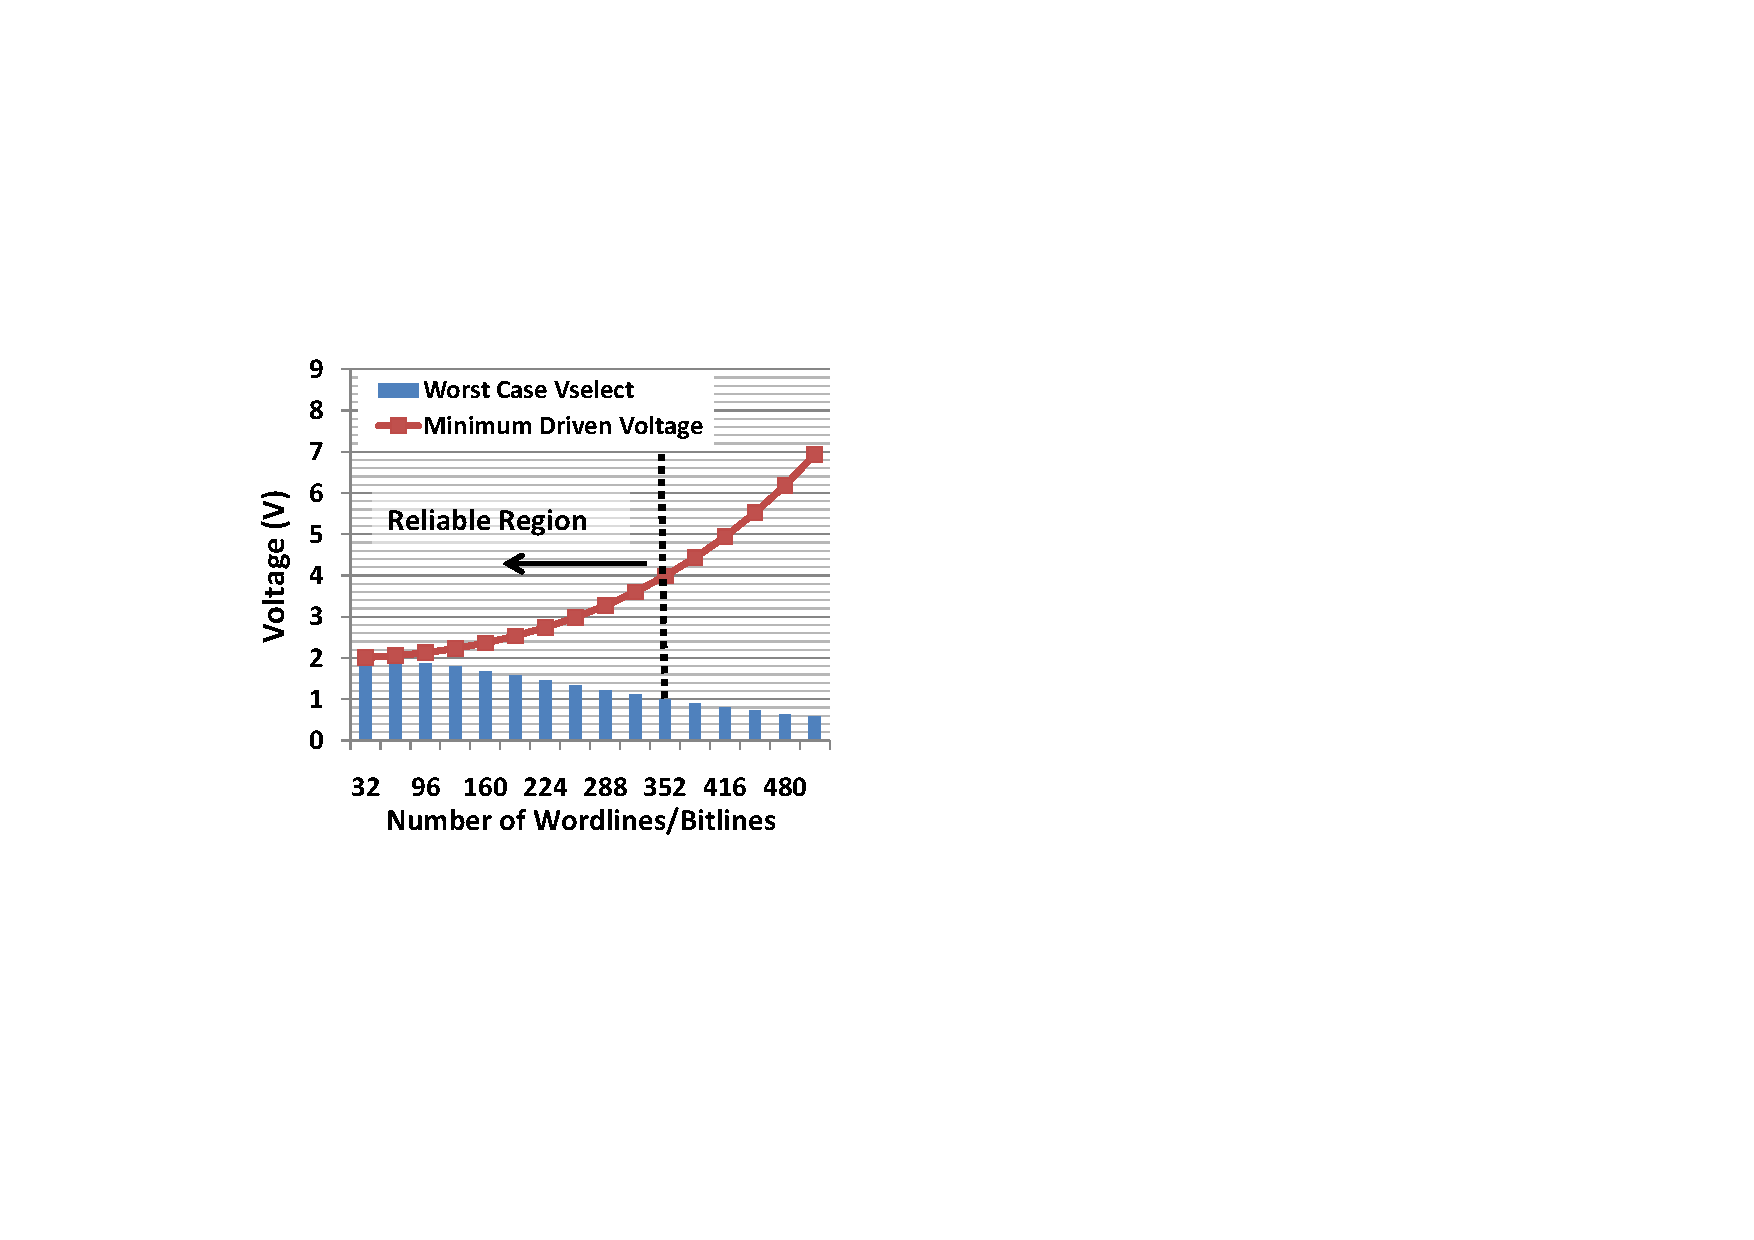
\includegraphics[width=0.25\textwidth]{./figures/multi_V_one.pdf}\\
  \caption{Worst case select voltage and write voltage requirements for multi-bit writing (one wordline per write).}\label{fig:reliable_region}
    \vspace{-10pt}
\end{figure}

\vspace{5pt}\noindent\textbf{Read Operation.} In this section we apply a
similar sensing scheme as \cite{crossbar_NANO08_Flocke} and
\cite{crossbar_TED_2010}. In order to read cell $R_{i,j}$, the $i^{th}$
wordline is biased at $V_{READ}$ and all of the other wordlines and
bitlines are grounded. Then the state of the selected cell is read out by
measuring the voltage across $R_s$. The energy consumption for a read
operation can be analyzed similarly as a write operation. Since the read
voltage is much smaller than write voltage, the read energy is expected to
be at least one order of magnitude smaller than for a write operation.
Considerable sensing margin is achieved by implementing a
current-to-voltage converter and sensing the voltage signal using
traditional or more recent sense amplifier designs. The input resistance
of the current-to-voltage converter is extracted from HSPICE simulation
results. Read sensing margin is defined as $\Delta V = \Delta I \times
R_{converter}$ where $R_{converter}$ is the input resistance of the
converter. The read reliability is determined by the voltage swing for
reading HRS and LRS cells.
%In order to improve the reliability of the read operation, a two-step sensing scheme can be applied~\cite{memristor:Cong}, which senses the current of an unselected cell first, then the overall current is sensed, and after that the current difference is converted to the output voltage.
Detailed results will be shown in Section~\ref{sec:scale}.

%Additionally, since the read voltage/current is much lower than the write voltage/current, we believe that the voltage drivers can always provide enough current for the read operation if they meet the current requirement for write operation. Therefore, we can conclude that the area overhead of voltage drivers is determined by the write current. However, the reliability of read operation is different from the write operation. Figure~\ref{fig:sense_margin_basic} (a) shows the voltage swing with different array sizes. Specifically, larger cross-point array have more sneak paths, making the output voltage very sensitive to the data pattern of unselected cell. Therefore, the sense margin decreases with the increase of array size.  The voltage swing of this two-step sensing scheme is shown in Figure~\ref{fig:sense_margin_basic} (b). By using this two-step sensing schemes, the voltage swing for a given array size and nonlinearity coefficient is doubled.


%\begin{figure}%[!t]
%\centering
%  % Requires \usepackage{graphicx}
%  \includegraphics[width=0.4\textwidth]{./figures/multi_I2.pdf}\\
%  \caption{The }\label{fig:multi_I}
%\end{figure}


%\subsection{Read Operation}
%In this section we applied the similar sensing scheme as
%\cite{crossbar_TED_2010} and \cite{crossbar_NANO08_Flocke}. In order to
%read cell $R_{i,j}$, the $i^{th}$ wordline is biased at $V_{READ}$ and all
%of the other wordlines and bitlines are grounded. Then the state of the
%selected cell is read out by measuring the voltage across $R_s$. The
%energy consumption for read operation can be analyzed by the same way as
%that of the write operation. Since the read voltage is much smaller than
%write voltage, the read energy is expected at least one order smaller than
%write operation. Additionally, since the read voltage/current is much
%lower than the write, we believe that the voltage drivers can always
%provide enough current for the read operation if they meet the current
%requirement for write operation. Therefore, we can conclude that the area
%overhead of voltage drivers is determined by the write current. However,
%the reliability of read operation is different from the write operation.
%The read reliability is determined by the voltage swing for reading HRS
%and LRS cells. Figure~\ref{fig:sense_margin} (a) shows the voltage swing
%with different array sizes and $K_r$ values. Large array sizes and large
%nonlinearity are harmful to the voltage swing: on the one hand, a larger
%array has more sneak paths, making the output voltage very sensitive to
%the data pattern of unselected cells; on the other hand, the nonlinearity
%increases the resistance of LRS and therefore the resistance difference
%between HRS and LRS cells is reduced. In order to improve the reliability
%of the read operation, a two-step sensing scheme can be applied, which
%senses the current of an unselected cell first, then the overall current
%is sensed, and after that the current difference is converted to the
%output voltage. The voltage swing of this two-step sensing scheme is shown
%in Figure~\ref{fig:sense_margin} (b). By using this two-step sensing
%schemes, the voltage swing for a given array size and nonlinearity
%coefficient is doubled.
%
%%\begin{figure}%[!t]
%%\centering
%%  % Requires \usepackage{graphicx}
%%  \includegraphics[width=0.45\textwidth]{./figures/margin.pdf}
%%  \caption{The}\label{fig:margin}
%%\end{figure}
%%
%%\begin{figure}%[!t]
%%\centering
%%  % Requires \usepackage{graphicx}
%%  \includegraphics[width=0.4\textwidth]{./figures/overlap.pdf}\\
%%  \caption{The}\label{fig:overlap}
%%\end{figure}
%
%%
%%\begin{figure}%[!t]
%%\centering
%%  % Requires \usepackage{graphicx}
%%  \includegraphics[width=0.5\textwidth]{./figures/sense_margin21}\\
%%  \caption{The}\label{fig:sense_margin}
%%\end{figure}
%
%\begin{figure}[!b]
%\centering
%  % Requires \usepackage{graphicx}
%  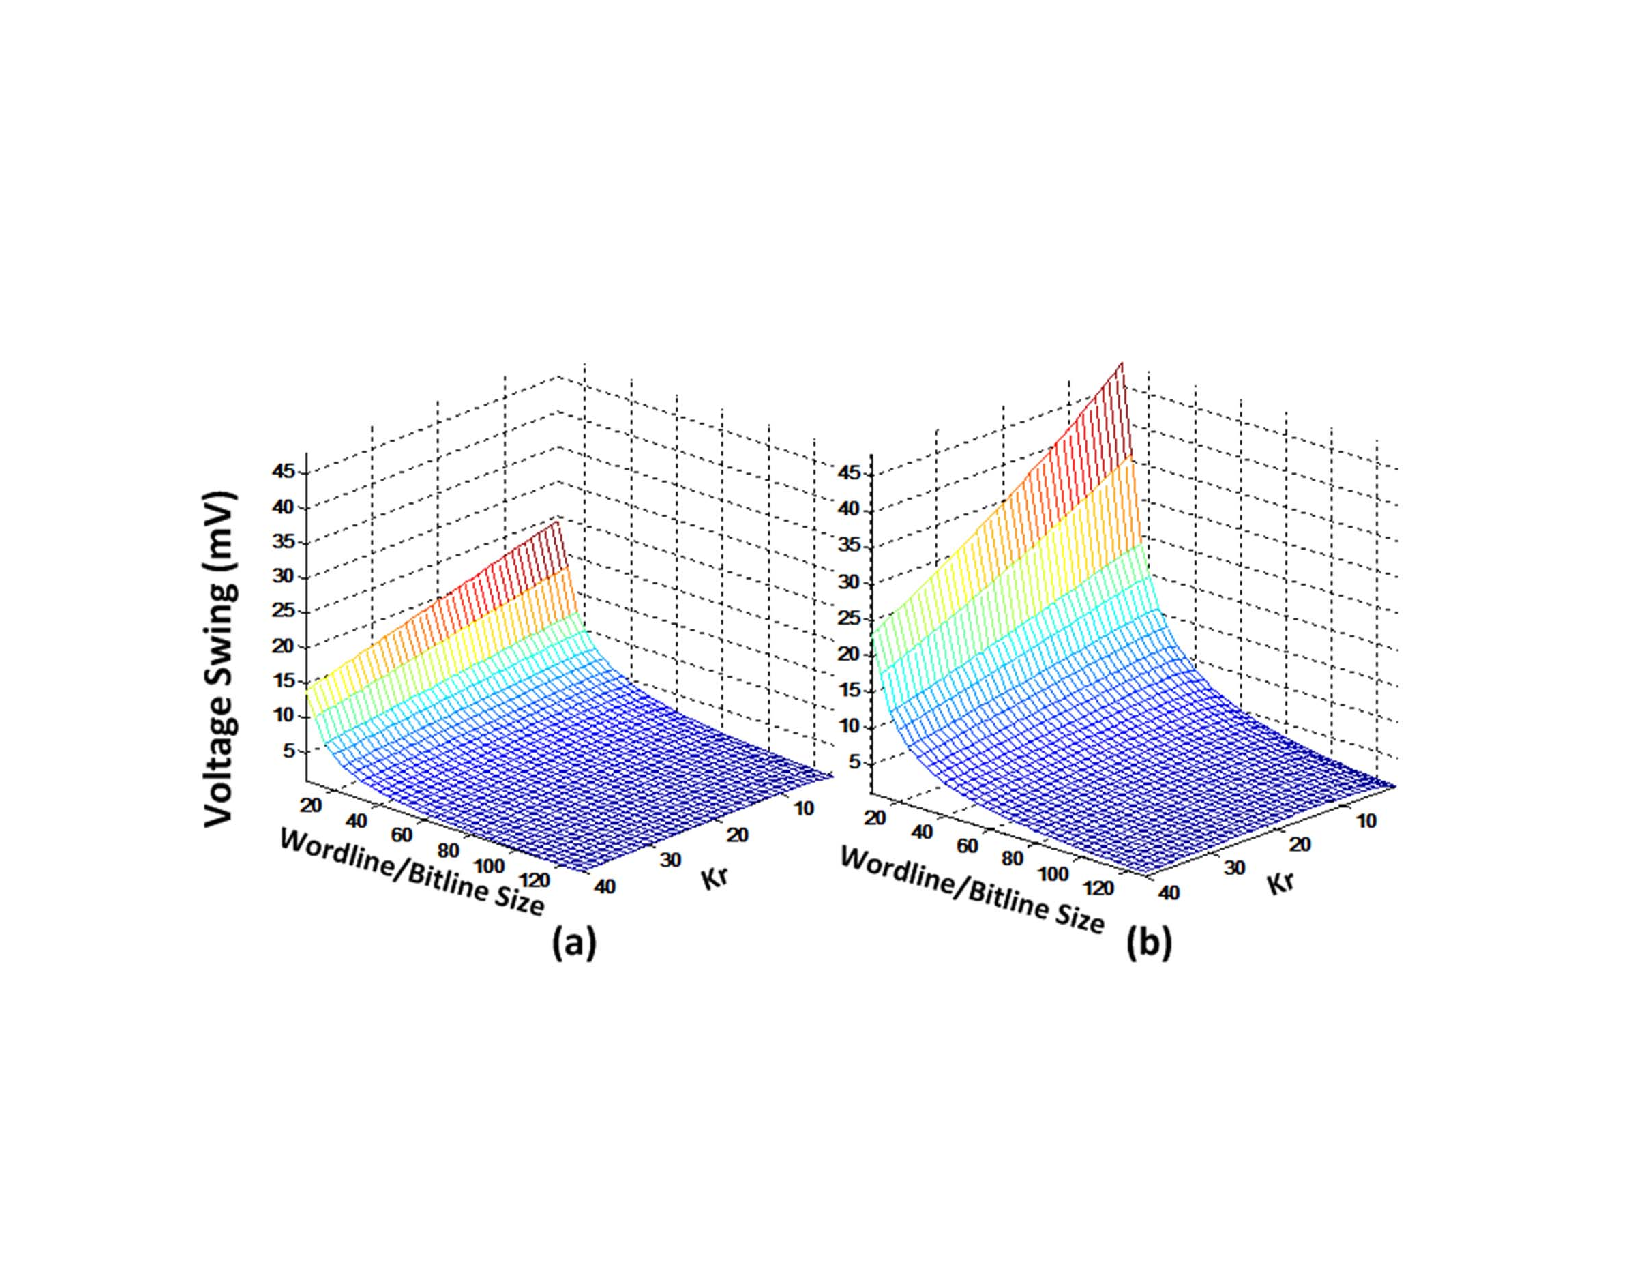
\includegraphics[width=0.5\textwidth]{./figures/sense_margin_f}\\
%  \caption{Relationships among the voltage swing, array size and nonlinearity. (a) Normal sensing scheme; (b) Two-step sensing scheme}\label{fig:sense_margin}
%\end{figure}

\vspace{-5pt}
\section{Nonlinearity and Write Current Scaling}\label{sec:scale}
\vspace{-2pt}
%\section{Nonlinearity and Write Current Scaling}\label{sec:scale}
%\subsection{Nonlinearity of the ReRAM Cell.} \vspace{6pt}
\begin{figure}[!b]
\centering
  \vspace{-5pt}
  % Requires \usepackage{graphicx}
  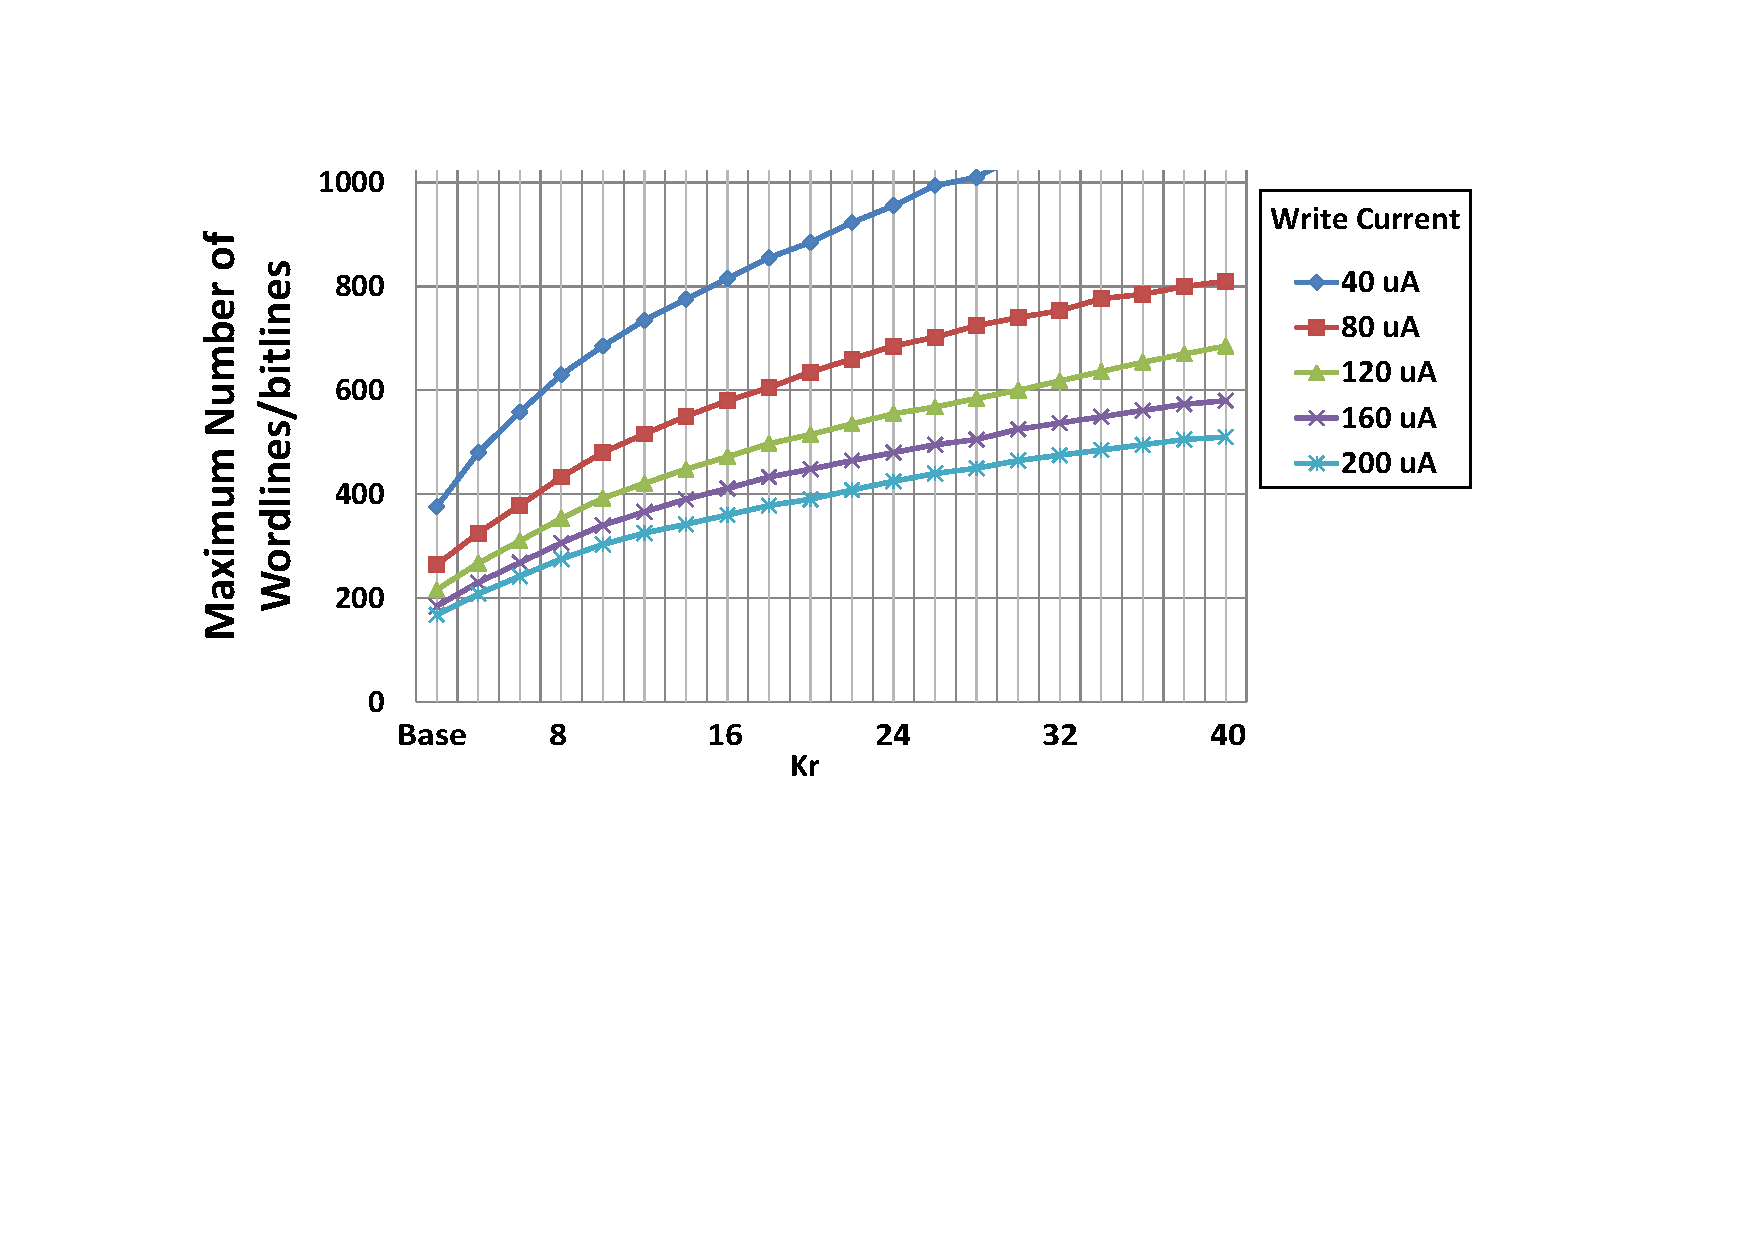
\includegraphics[width=3.3in]{./figures/non_linear_f}\\
  \vspace{-10pt}
  \caption{The maximum array size with different nonlinearity coefficients.}\label{fig:non_linear}
\end{figure}
One of the most distinct features of ReRAM is its nonlinearity. Normally,
the $K_r$ value for memristor-based ReRAM is larger than 20, meaning that
the resistance of a half-biased cell is at least 10 times larger than a
full-biased cell. Clearly, ReRAM cells with larger nonlinearity
coefficients result in a better memory cell since the sneak current in
half selected cells will be significantly reduced. In addition, the
increased resistance at half-selected and unselected cells can also
mitigate the voltage drop along the activated wordline and bitline. Also,
we find that the cross-point array design can benefit from the scaling of
the write current. Figure~\ref{fig:non_linear} shows the influence of
different nonlinearity coefficients and write currents on the array size
requirements for a single-bit HWHB writing scheme. This figure shows that
the array size limitation is relaxed as the nonlinearity increases or the
write current scales. As we can see from the figure, the maximum array
size exceeds $1024\times 1024$ when we have a nonlinearity of $30$,
together with a write current of $40\mu A$.

Moreover, the increase of nonlinearity or scaling of write current can
also reduce the energy consumption and area overhead of the cross-point
array. As shown in Figure~\ref{fig:E_and_A}(a), for a $512 \times 512$
array, the energy consumption for the write operation decreases
dramatically with the scaling of nonlinearity coefficient $K_r$. For
example, for a ReRAM cell with write current of 50uA, the write energy is
reduced by 98.3\% when $K_r$ increases from 2 to 40. The area overhead of
the voltage drivers is illustrated in Figure~\ref{fig:E_and_A}(b). As a
baseline design ($K_r=20$ and $I_w=40\mu A$), the driver area overhead is
about 35\% of the area of the memory array cells. To design a memory array
with an effective cell size close to $4F^2$, we need to make sure the
nonlinearity and write current should satisfy certain conditions so that
the driver overhead is less than 100\% and the wordline drivers can be
almost ``hidden'' underneath the ReRAM cells. As nonlinearity and write
current continues to scale, the area overhead can be as low as 10\%. In
that case, the introduction of 3D stacking of multi-layer cross-point
arrays is productive in further reducing the effective cell size to $4/N_l
F^2$ where $N_l$ is the number of layers.

%Therefore, we can conclude that, the ReRAM cells with a small nonlinearity coefficient are not suitable for the cross-point structure based memory array. Next, we study the area overhead of multi-bit write. Figure~\ref{fig:Area_kr20} shows the normalized areas of the voltage drivers for one bit and multi-bit write operations. As mentioned, multi-bit write operations require larger drive current. Therefore, the area of voltage drivers for multi-bit write operations are much larger than that for one bit write operations. Finally, normalized areas of the one bit and multi-bit write operations have opposite trends as the array size increases. Normalized area for one bit write operation increases with the array size. On the contrary, normalized area for multi-bit write decreases as the array size increase.}

%\begin{figure}%[!t]
%\centering
%  % Requires \usepackage{graphicx}
%  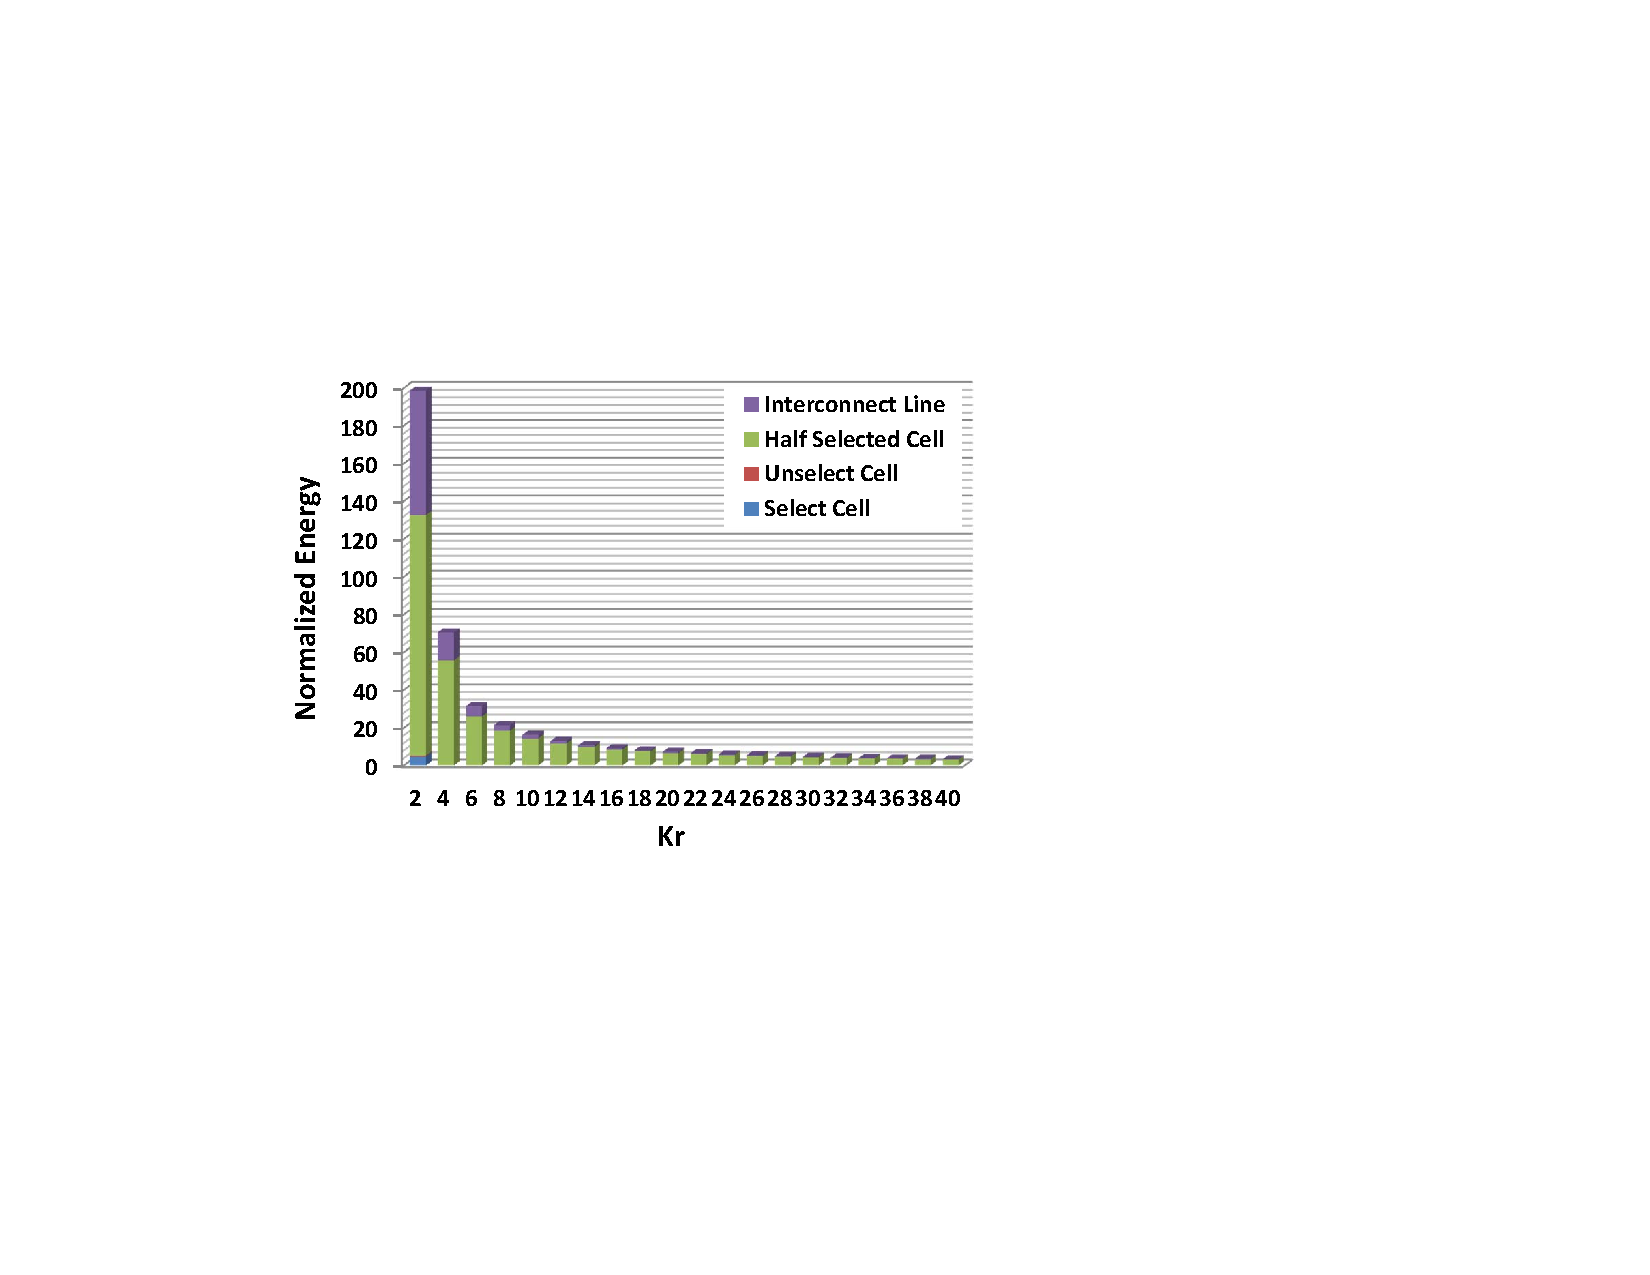
\includegraphics[width=0.38\textwidth]{./figures/non_linear_energy.pdf}\\
%  \caption{The normalized energy consumption with nonlinear ReRAM cells.}\label{fig:non_linear_energy}
%\end{figure}

%\begin{figure}%[!t]
%\centering
%  % Requires \usepackage{graphicx}
%  \includegraphics[width=0.4\textwidth]{./figures/non_linear_I.pdf}\\
%  \caption{The}\label{fig:non_linear_I}
%\end{figure}
%
%\begin{figure}%[!t]
%\centering
%  % Requires \usepackage{graphicx}
%  \includegraphics[width=0.4\textwidth]{./figures/non_linear_ara.pdf}\\
%  \caption{The}\label{fig:non_linear_ara}
%\end{figure}
%\begin{figure}%[!t]
%\centering
%  % Requires \usepackage{graphicx}
%  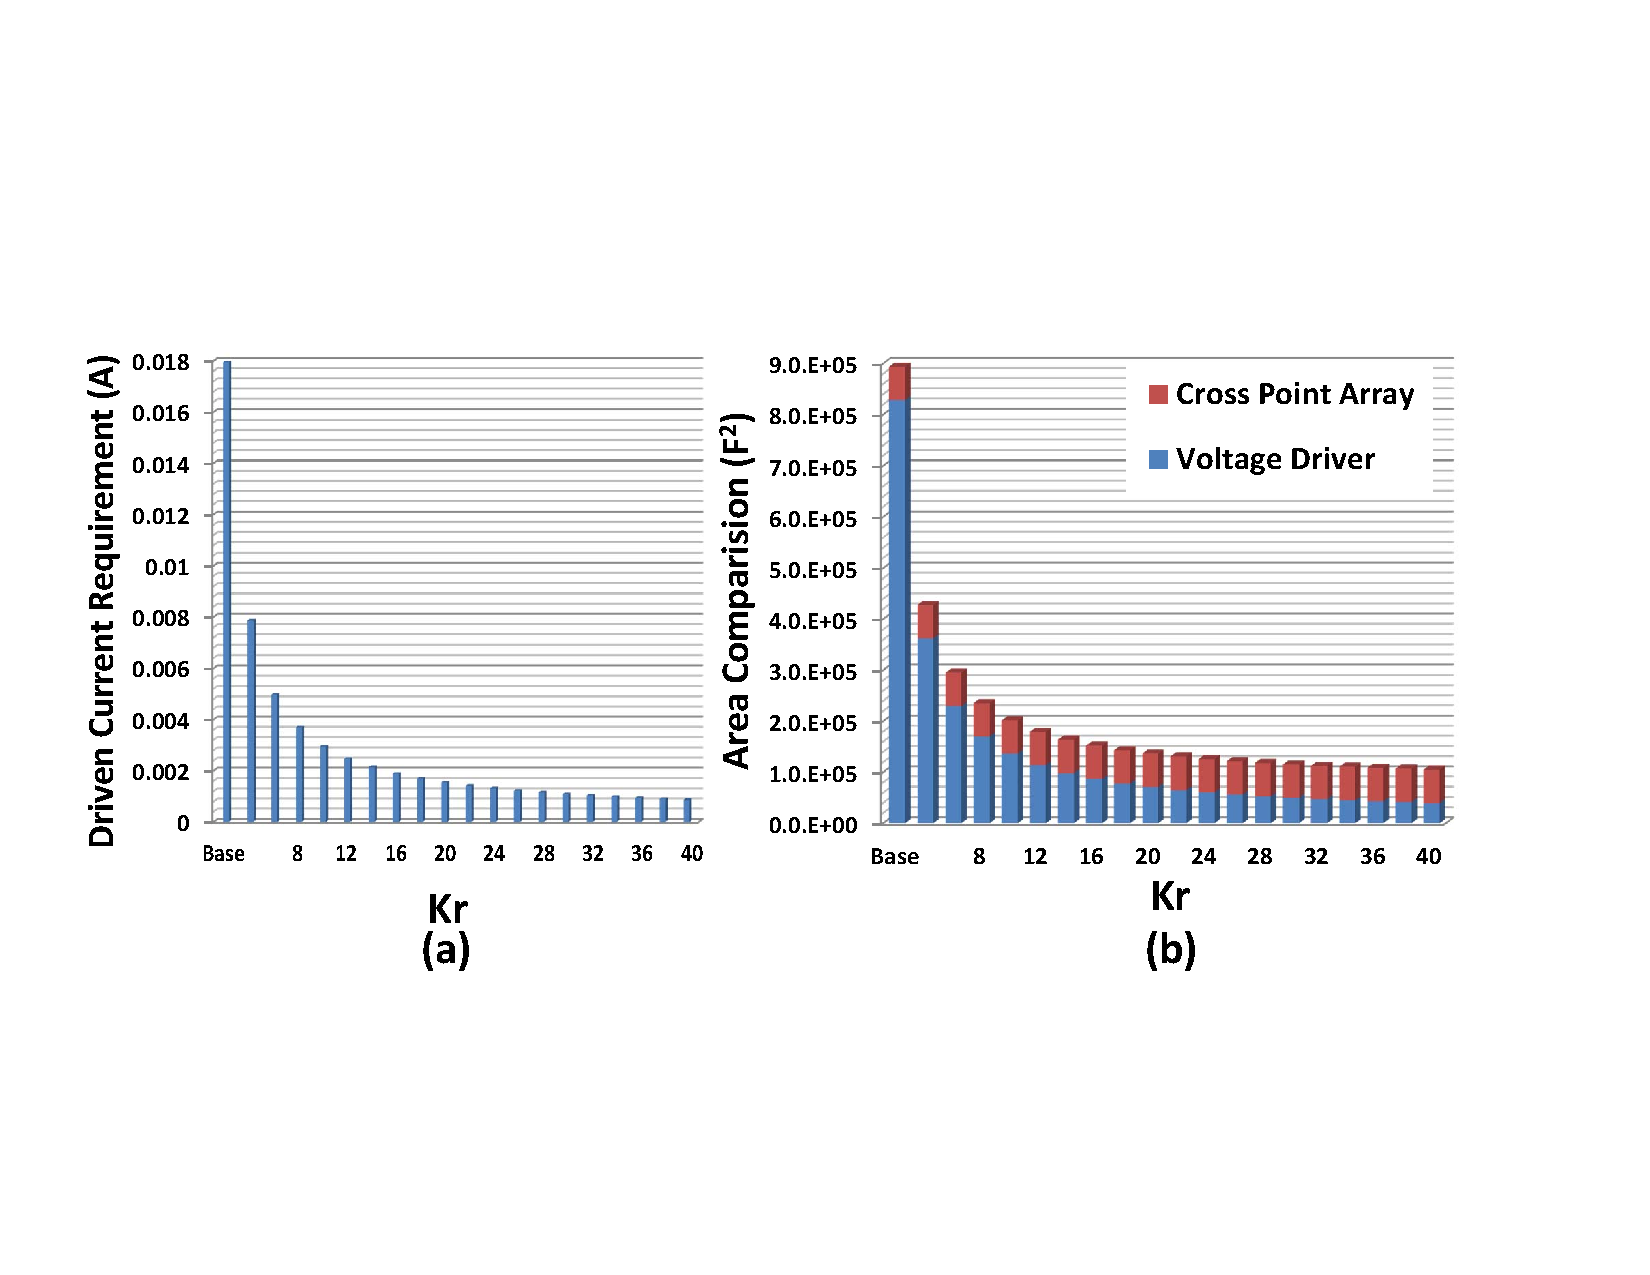
\includegraphics[width=0.5\textwidth]{./figures/area_all.pdf}\\
%  \vspace{-5pt}
%  \caption{The driven current requirements and area overheads with different nonlinearity coefficients}\label{fig:area_all}
% \vspace{-15pt}
%\end{figure}
\begin{figure}[!t]
\centering
  % Requires \usepackage{graphicx}
  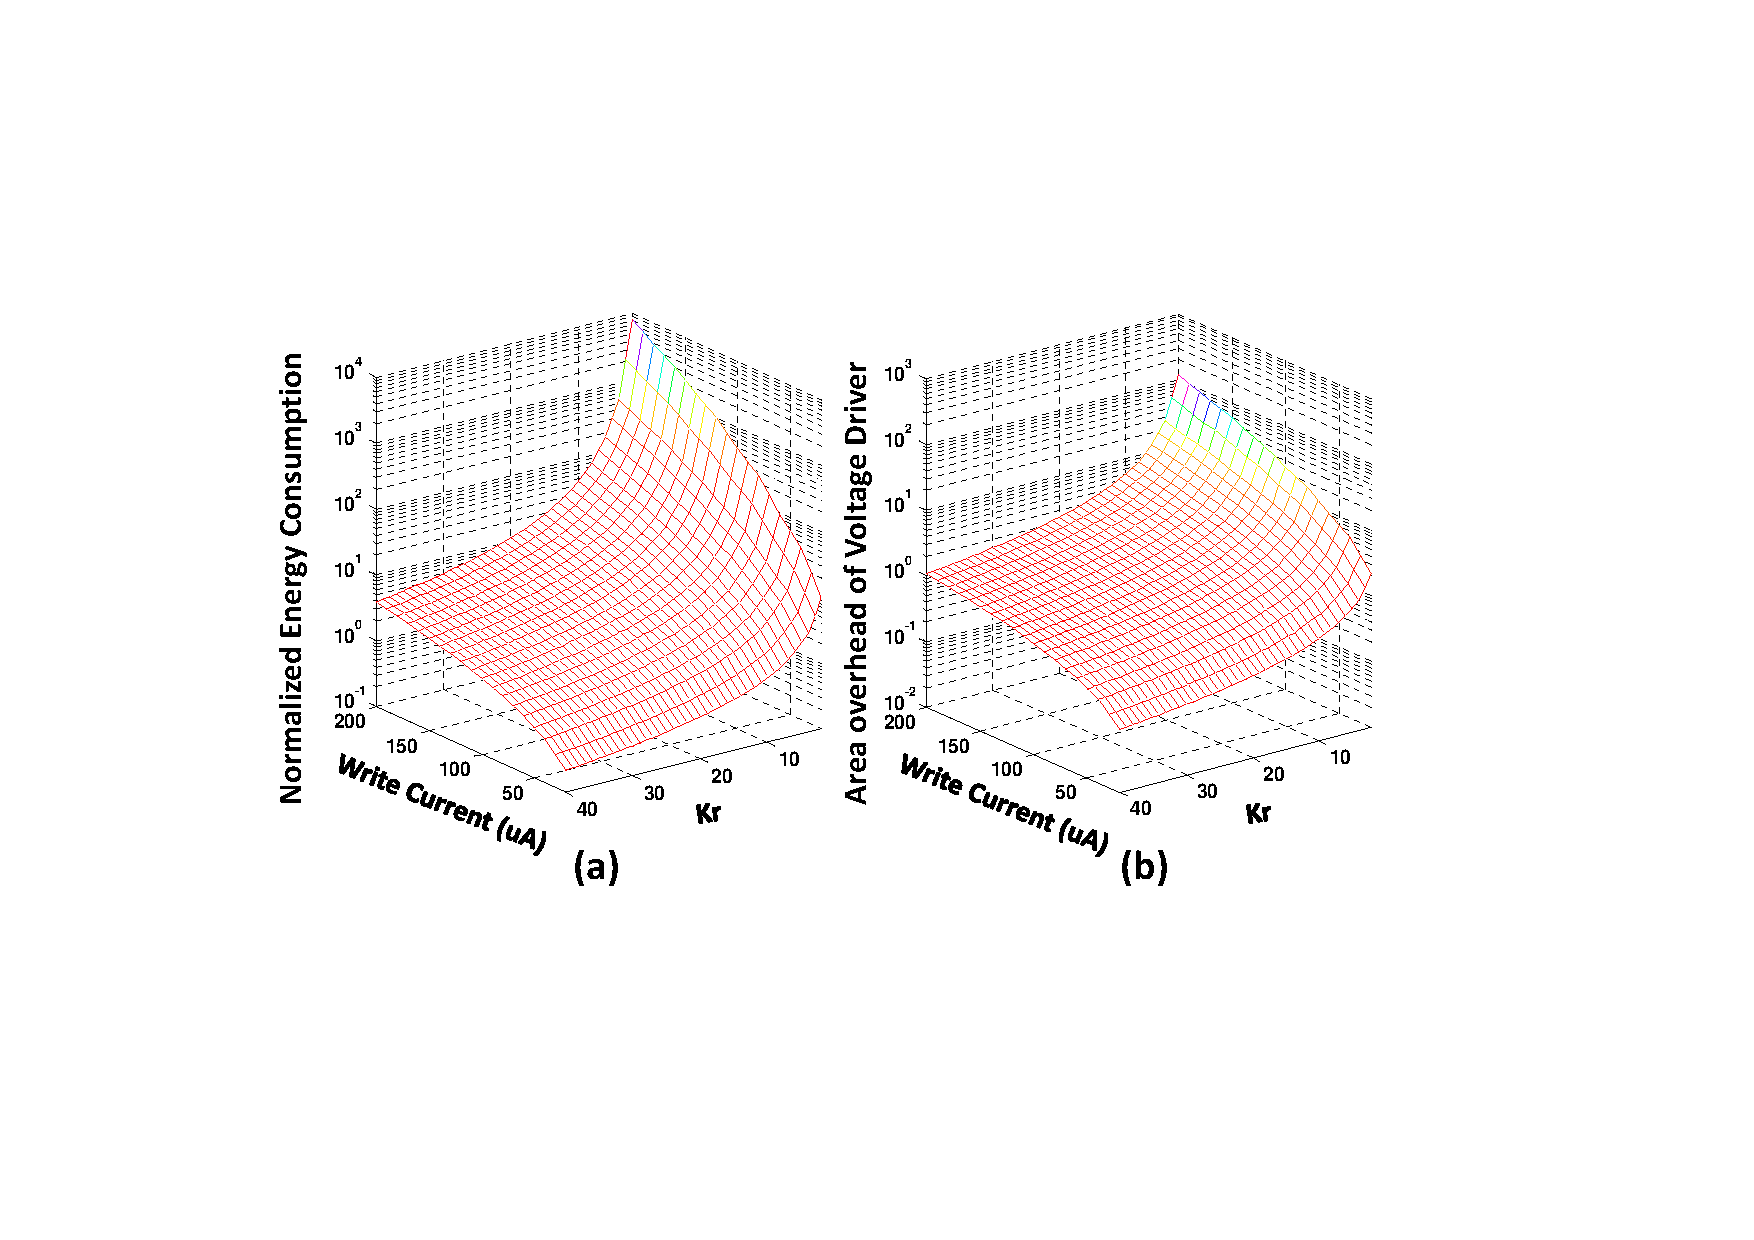
\includegraphics[width=0.45\textwidth]{./figures/E_and_A}\\
\vspace{-5pt}
  \caption{Energy and area overhead comparison. (a) Energy consumption (normalized to baseline). (b) Area overhead of voltage driver (normalized to the area of cross-point array).}\label{fig:E_and_A}
\vspace{-10pt}
\end{figure}

%\begin{figure}%[!t]
%\centering
%  % Requires \usepackage{graphicx}
%  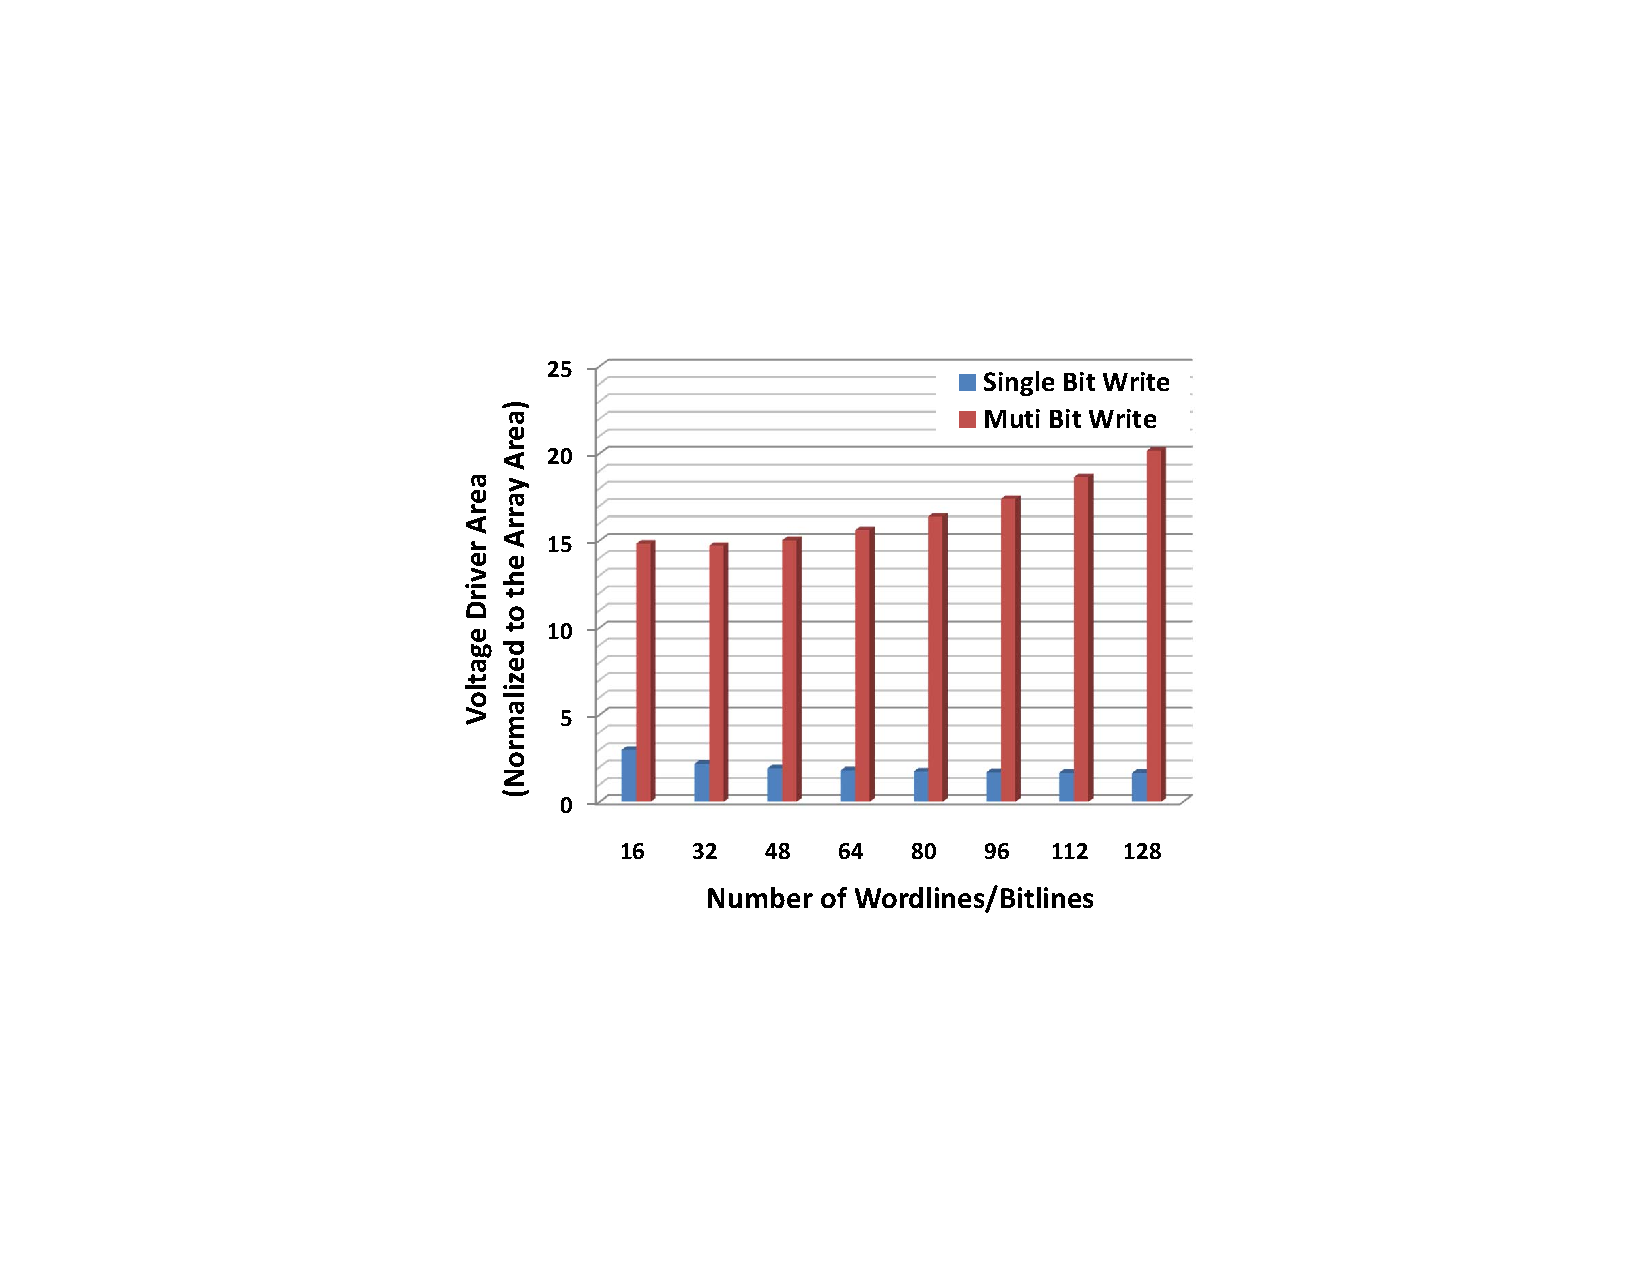
\includegraphics[width=0.35\textwidth]{./figures/Area_kr20_f.pdf}\\
%  \caption{The normalized area overhead of voltage drivers ($K_r=20$, the areas are normalized to the area of cross-point array). }\label{fig:Area_kr20}
%\end{figure}

Unlike the write operation, the read operation suffers, rather than
benefits, from scaling of nonlinearity or write current. This is because
the scaling of nonlinearity and write current will reduce read current,
degrading the read signal ratio. Figure~\ref{fig:sense_margin}(a) shows
the read noise margin with different array sizes for the baseline design
in Section~\ref{sec:w_and_r}.  As can be seen, the read noise margin is
reduced for large array sizes. The impact of nonlinearity and write
current on read noise margin is illustrated in
Figure~\ref{fig:sense_margin}(b). A large $K_r$ value and small write
current are harmful to the read noise margin. For example, given a $512
\times 512$ array, the read noise margin is less than $10mV$ for $K_r=40$
and $I_w=40\mu A$, which makes it very difficult to sense the state of the
selected memory cell using traditional sense amplifiers.

%the nonlinearity increases the resistance of half LRS and therefore the
%resistance difference between HRS and LRS cells is reduced; on the other
%hand, .
\begin{figure}[!t]
\centering
  % Requires \usepackage{graphicx}
  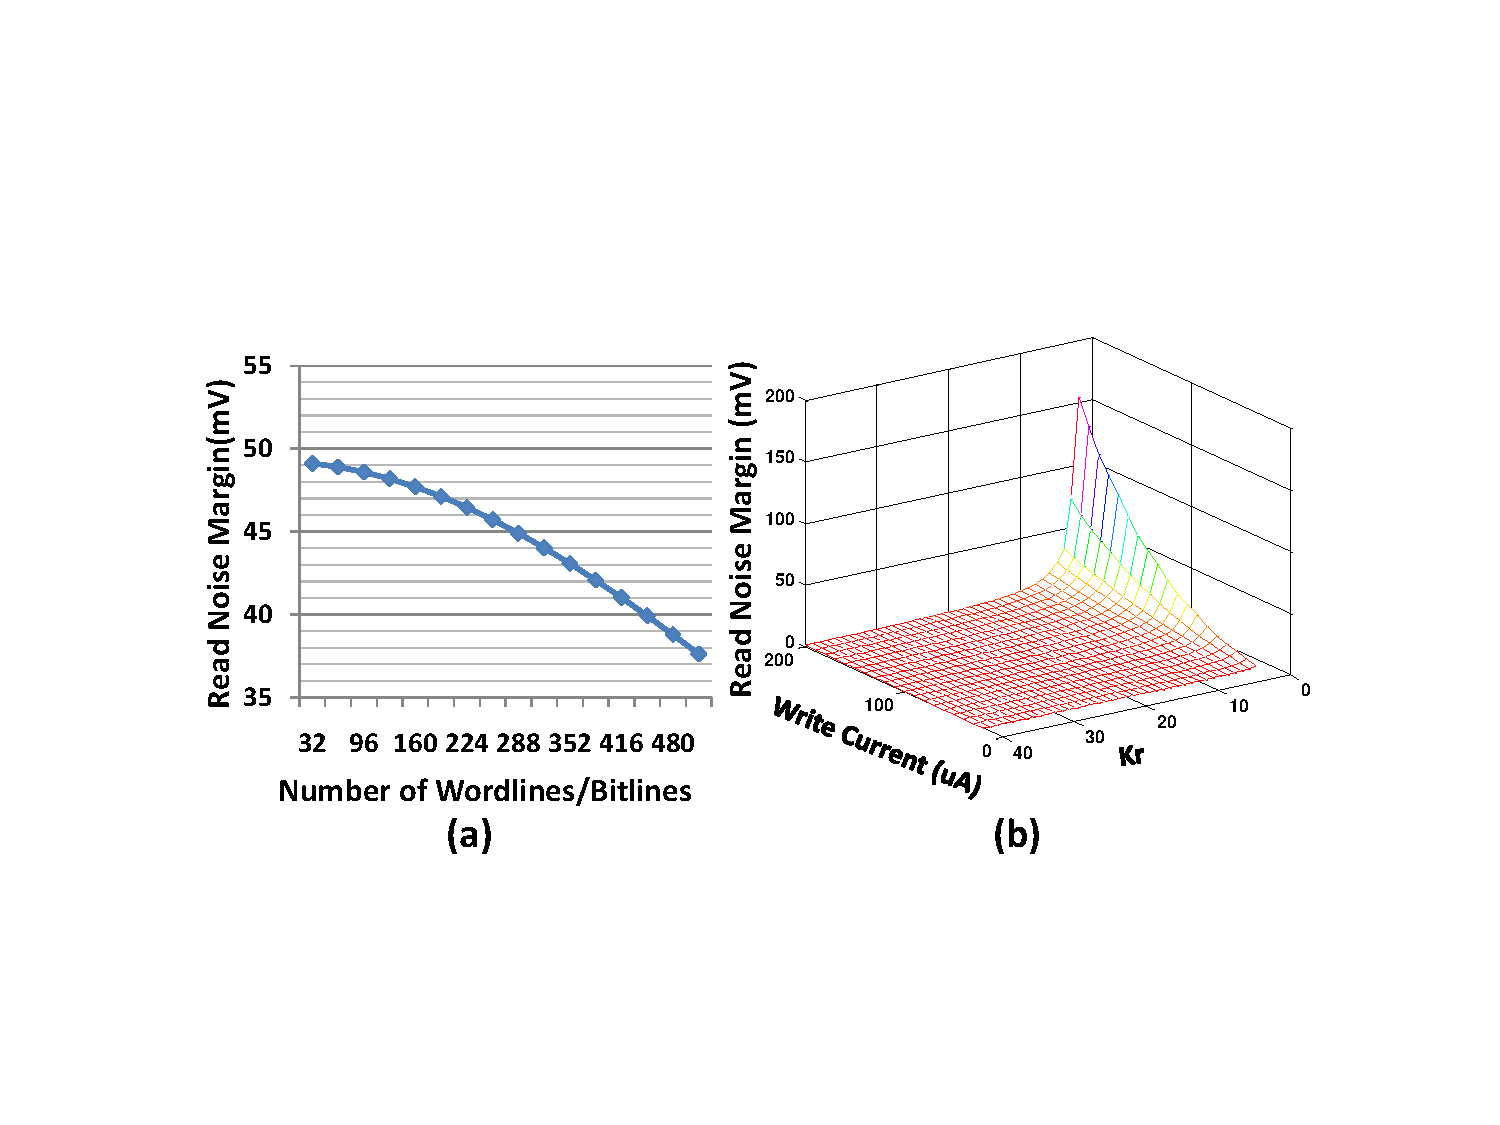
\includegraphics[width=0.45\textwidth]{./figures/read}\\\vspace{-5pt}
  \caption{Read noise margin with (a) different array size and (b) scaling of nonlinearity and write current.}\label{fig:sense_margin}
  \vspace{-15pt}
\end{figure}

Therefore, by knowing the array size and read noise margin constraints, an
``optimal cell'' with nonlinearity of $K_{r\_opt}$ and write current of
$I_{on\_opt}$ can be determined. For example, when the array size is fixed
at $512 \times 512$ and the minimum noise margin is $50mV$, a cross-point
array with ReRAM cells which have $K_{r\_opt} = 9$ and $I_{on\_opt} =
40mA$ is the most energy and area efficient design.


%\subsection{Read Operation}
%In this section we applied the similar sensing scheme as
%\cite{crossbar_TED_2010} and \cite{crossbar_NANO08_Flocke}. In order to
%read cell $R_{i,j}$, the $i^{th}$ wordline is biased at $V_{READ}$ and all
%of the other wordlines and bitlines are grounded. Then the state of the
%selected cell is read out by measuring the voltage across $R_s$. The
%energy consumption for read operation can be analyzed by the same way as
%that of the write operation. Since the read voltage is much smaller than
%write voltage, the read energy is expected at least one order smaller than
%write operation. Additionally, since the read voltage/current is much
%lower than the write, we believe that the voltage drivers can always
%provide enough current for the read operation if they meet the current
%requirement for write operation. Therefore, we can conclude that the area
%overhead of voltage drivers is determined by the write current. However,
%the reliability of read operation is different from the write operation.
%The read reliability is determined by the voltage swing for reading HRS
%and LRS cells. Figure~\ref{fig:sense_margin} (a) shows the voltage swing
%with different array sizes and $K_r$ values. Large array sizes and large
%nonlinearity are harmful to the voltage swing: on the one hand, a larger
%array has more sneak paths, making the output voltage very sensitive to
%the data pattern of unselected cells; on the other hand, the nonlinearity
%increases the resistance of LRS and therefore the resistance difference
%between HRS and LRS cells is reduced. In order to improve the reliability
%of the read operation, a two-step sensing scheme can be applied, which
%senses the current of an unselected cell first, then the overall current
%is sensed, and after that the current difference is converted to the
%output voltage. The voltage swing of this two-step sensing scheme is shown
%in Figure~\ref{fig:sense_margin} (b). By using this two-step sensing
%schemes, the voltage swing for a given array size and nonlinearity
%coefficient is doubled.
%
%
%
%\begin{figure}[!t]
%\centering
%  % Requires \usepackage{graphicx}
%  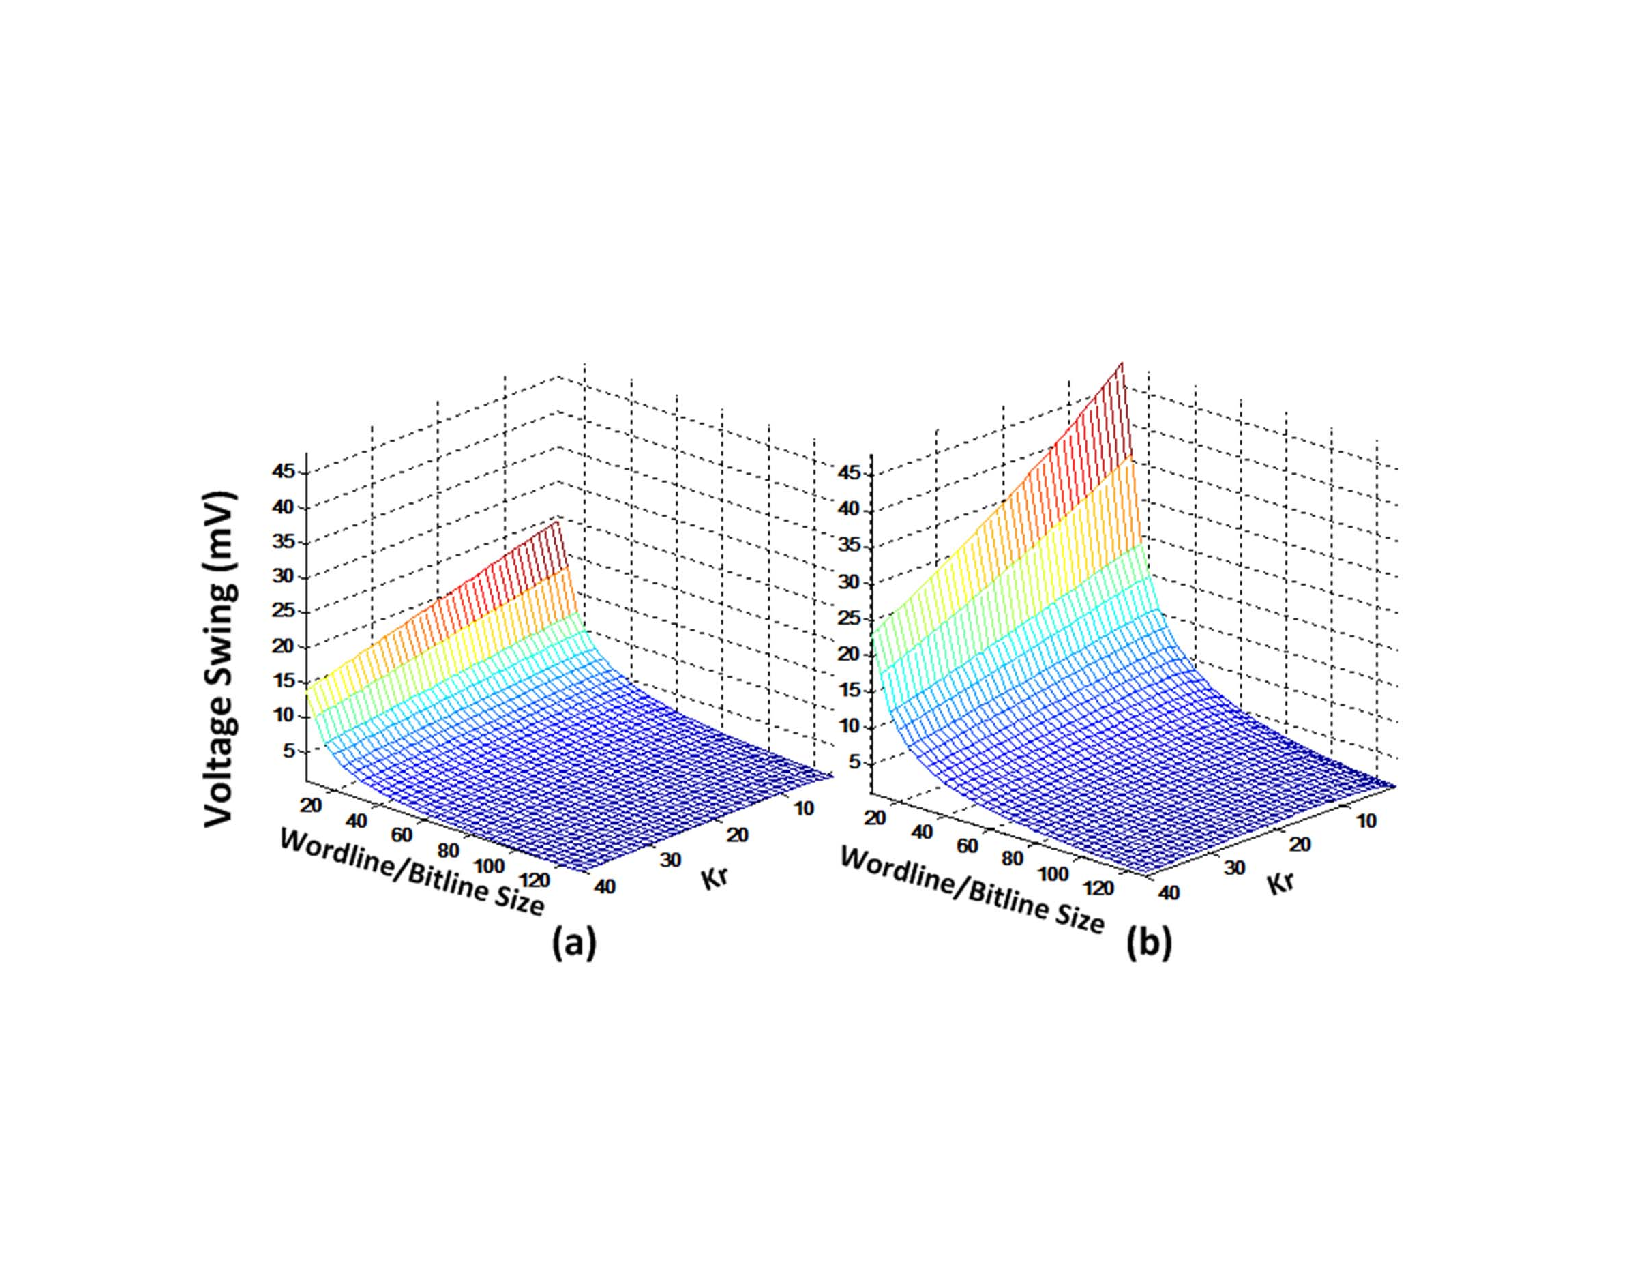
\includegraphics[width=0.5\textwidth]{./figures/sense_margin_f}\\
%  \caption{Relationships among the voltage swing, array size and nonlinearity. (a) Normal sensing scheme; (b) Two-step sensing scheme}\label{fig:sense_margin}
%\end{figure}


\begin{table*}
\label{tab:results} \caption{Area, energy, and bandwidth results of 256
Mbits ReRAM macro} \vspace{-8pt}
\begin{center}
\begin{tabular}{|c|c|c|r|r|r|r|r|r|r|r|}
\hline
\multirow{2}{*}{{$Kr$}} & \multirow{2}{*}{{$I_w(uA)$}} & \multirow{2}{*}{\bf{~~~~}}& \multicolumn{8}{|c|}{{Number of bit per write at array level}} \\ \cline{4-11}
& &  & \multicolumn{1}{|c|}{1} & \multicolumn{1}{|c|}2 & \multicolumn{1}{|c|}4 & \multicolumn{1}{|c|}8 & \multicolumn{1}{|c|}{16} & \multicolumn{1}{|c|}{32} & \multicolumn{1}{|c|}{64} & \multicolumn{1}{|c|}{128} \\ \hline
\multirow{3}{*}{{20}}& \multirow{3}{*}{{40}} & {{Area(mm$^2$)}} &	3.888	&	3.944	&	4.056	&	4.288	&	4.752	&	5.688	&	7.544	&	11.752	\\ \cline{3-11}
&  & {{Energy(nJ)}} &	4.375	&	12.379	&	19.860	&	33.660	&	59.430	&	111.404	&	232.437	&	576.496	\\ \cline{3-11}
&  & {{Bandwidth(MBit/s)}} &	66.687	&	72.618	&	144.747	&	287.534	&	567.290	&	1103.991	&	2089.847	&	3649.583	\\\hline
\multirow{3}{*}{{20}}& \multirow{3}{*}{{200}} & {{Area(mm$^2$)}} &	6.512	&	6.816	&	7.424	&	8.640	&	11.096	&	16.144	&	27.288	&	\multicolumn{1}{|c|}{N/A}	\\ \cline{3-11}
&  & {{Energy(nJ)}} &	24.584	&	67.126	&	106.848	&	182.409	&	338.781	&	716.141	&	1845.355	&	\multicolumn{1}{|c|}{N/A}	\\ \cline{3-11}
&  & {{Bandwidth(MBit/s)}} &	90.038	&	113.028	&	217.351	&	401.199	&	685.218	&	1018.788	&	1213.958	&	\multicolumn{1}{|c|}{N/A}	\\\hline
\multirow{3}{*}{{40}}& \multirow{3}{*}{{40}} & {{Area(mm$^2$)}} &	3.616	&	3.672	&	3.776	&	3.992	&	4.752	&	5.688	&	7.544	&	11.432	\\ \cline{3-11}
&  & {{Energy(nJ)}} &	2.065	&	5.550	&	8.711	&	14.485	&	25.601	&	49.322	&	107.519	&	280.121	\\ \cline{3-11}
&  & {{Bandwidth(MBit/s)}} &	69.594	&	74.309	&	148.111	&	294.199	&	580.357	&	1129.126	&	2136.164	&	3777.482	\\\hline
\multirow{3}{*}{{40}}& \multirow{3}{*}{{200}} & {{Area(mm$^2$)}} &	3.984	&	4.288	&	4.888	&	6.088	&	8.464	&	13.328	&	24.088	&	\multicolumn{1}{|c|}{N/A}	\\ \cline{3-11}
&  & {{Energy(nJ)}} &	11.645	&	29.739	&	46.939	&	80.813	&	155.025	&	343.658	&	933.231	&	\multicolumn{1}{|c|}{N/A}	\\ \cline{3-11}
&  & {{Bandwidth(MBit/s)}} &	115.781	&	131.827	&	253.686	&	469.243	&	800.280	&	1174.237	&	1362.144	&	\multicolumn{1}{|c|}{N/A}	\\\hline
\end{tabular}
\vspace{-12pt}
\end{center}
\end{table*}

\vspace{-5pt}
\section{A Case Study of Cross-point ReRAM Macro Design}\label{sec:macro}
Since the array size of a cross-point ReRAM array is limited by
the reliability requirements, the design of a ReRAM macro is different
from the traditional DRAM design. 
%A cross-point ReRAM macro is implemented
%by connecting a number of small cross-point arrays with
%appropriate peripheral circuity and organizations. 
In this section, we evaluate the area, energy consumption, and bandwidth of a
256 Mbits ReRAM macro.
We use an organization similar to Kawahara's design~\cite{crossbar_Panasonic}, where
%We apply the similar memory organization as Kawahara's
%work~\cite{crossbar_Panasonic}. 
a 256 Mbits ReRAM macro is divided into 
eight planes. Each 32~Mbit plane has separate wordline
decoder, bitline selectors, sense amplifiers, and write circuity. Due to
space constraints, we present results for only
four typical cell parameters: ($Kr=20,
I_w=40uA$), ($Kr=20, I_w=200uA$), ($Kr=40, I_w=40uA$), and ($Kr=40,
I_w=200uA$). For each of them, we vary the number of bit per write to
investigate the relation among the area, energy consumption, and bandwidth
of the ReRAM macro.


%Figure~\ref{fig:aaable}
Table~II shows the total area, energy consumption, and bandwidth of the
256 Mbits ReRAM macro. Consistent with our earlier discussion, 
as the device nonlinearity improves, both the area and energy 
overhead goes down. The only downside is the noise margin restriction
imposed for reads. Similarly, as the drive current increases, the overhead
goes up due to large wordline drivers and bitline multiplexors. 
In summary, it is clear that increased bandwidth comes at the cost of area
and energy. 

To better understand the ideal design choice for a given device parameter,
we investigated three metrics: bandwidth per
nanojoule ($BW/nJ$), bandwidth per square millimeter($BW/mm^2$), and
bandwidth per nanojoule per square millimeter ($BW/(nJ\cdot mm^2)$).
Figure~\ref{fig:BWpAE}~(a) shows how $BW/mm^2$ scale as we increase the 
number of bits modified per write operation. From the figure, for a given
energy budget, writing one bit at a time provides at least~48\% better bandwidth 
compared to the best performing muti-bit writes. Hence, with the right choice
of global interconnect, interleaving writes across multiple sub-arrays is
an interesting design point. 
With multi-bit writes, as the number of bits per write increases, the energy
efficiency also increases. However, as the word size increases, the voltage
drop in the array also increases, which needs to be compensated by increasing
the operating voltage of the array (Section~\ref{sec:w_and_r}). Beyond 32~bits, this
increase in voltage, outweighing the bandwidth improvement, effectively reducing
the energy efficiency.
Thus from energy standpoint, multi-bit write is optimal when the word size is
8-32~bits, depending upon the nonlinearity and drive current. 
Figure~\ref{fig:BWpAE}~(b) shows the effect of multi-bit writes on bandwidth per
square millimeter. Unlike energy, as long as the drive current is less, 
it is beneficial to increase the word size as much as possible to improve
bandwidth for a given area. Also, writing one bit at a time is the least 
attractive option for a design primarily constrained by the area.
Figure~\ref{fig:BWpAE2} takes into account both energy and area, and 
provides a ``sweet spot'' for multi-bit writes.
Thus by understanding the key characteristics of cross-point array, we can 
identify an optimal configuration that best meets the design constrains. 

%Bandwidth per nanojoule reflects the energy efficiency on the bandwidth.
%The higher the bandwidth and the less amount of energy used to achieve a
%larger values of this metric. Besides, since the area is directly related
%to the cost, bandwidth per square millimeter is a good indicator of the
%economics of the bandwidth. As shown in Figure~\ref{fig:BWpAE} the
%bandwidth per nanojoule for single-bit write is always better than that
%for multi-bit write operation. Besides, there also exist a optimal number
%of bits per write for multi-bit write schemes: 32 bits for the cell with
%Kr=20, and 8 bits for cells with Kr=40. However, from the bandwidth per
%square millimeter point of view, the cells with different write current
%have different situation: for cells with large write current
%($I_w=200uA$), optimal number of bits per write is 16 bits. On the other
%hand, if the write current scales to $40uA$, the bandwidth per square
%millimeter increases monotonically with the increase of write bit number,
%and the large number of bit per write is favorable. The reason for this
%different is that, for the cell with large write current, the wordline
%drivers and bitline multiplexors can no longer be hidden underneath the
%array, which impact the area efficiency of the entire macro.
%Figure~\ref{fig:BWpAE2} shows the bandwidth per nanojoule per square
%millimeter results. Similarly, this metric also has a optimal number of
%bits per write for different cells: 8 bits for the cell with Kr=20, and 4
%bits for cells with Kr=40. However, we should note that, even for the same
%ReRAM cell, the ``sweet spot'' for different metric is different.
%Therefore, we can conclude that the optimal configuration varies with the
%optimization target($BW/nJ$, $BW/mm^2$, or $BW/(nJ\cdot mm^2)$).

%\begin{figure}[!t]
%\centering\label{fig:aaable}
%  % Requires \usepackage{graphicx}
%  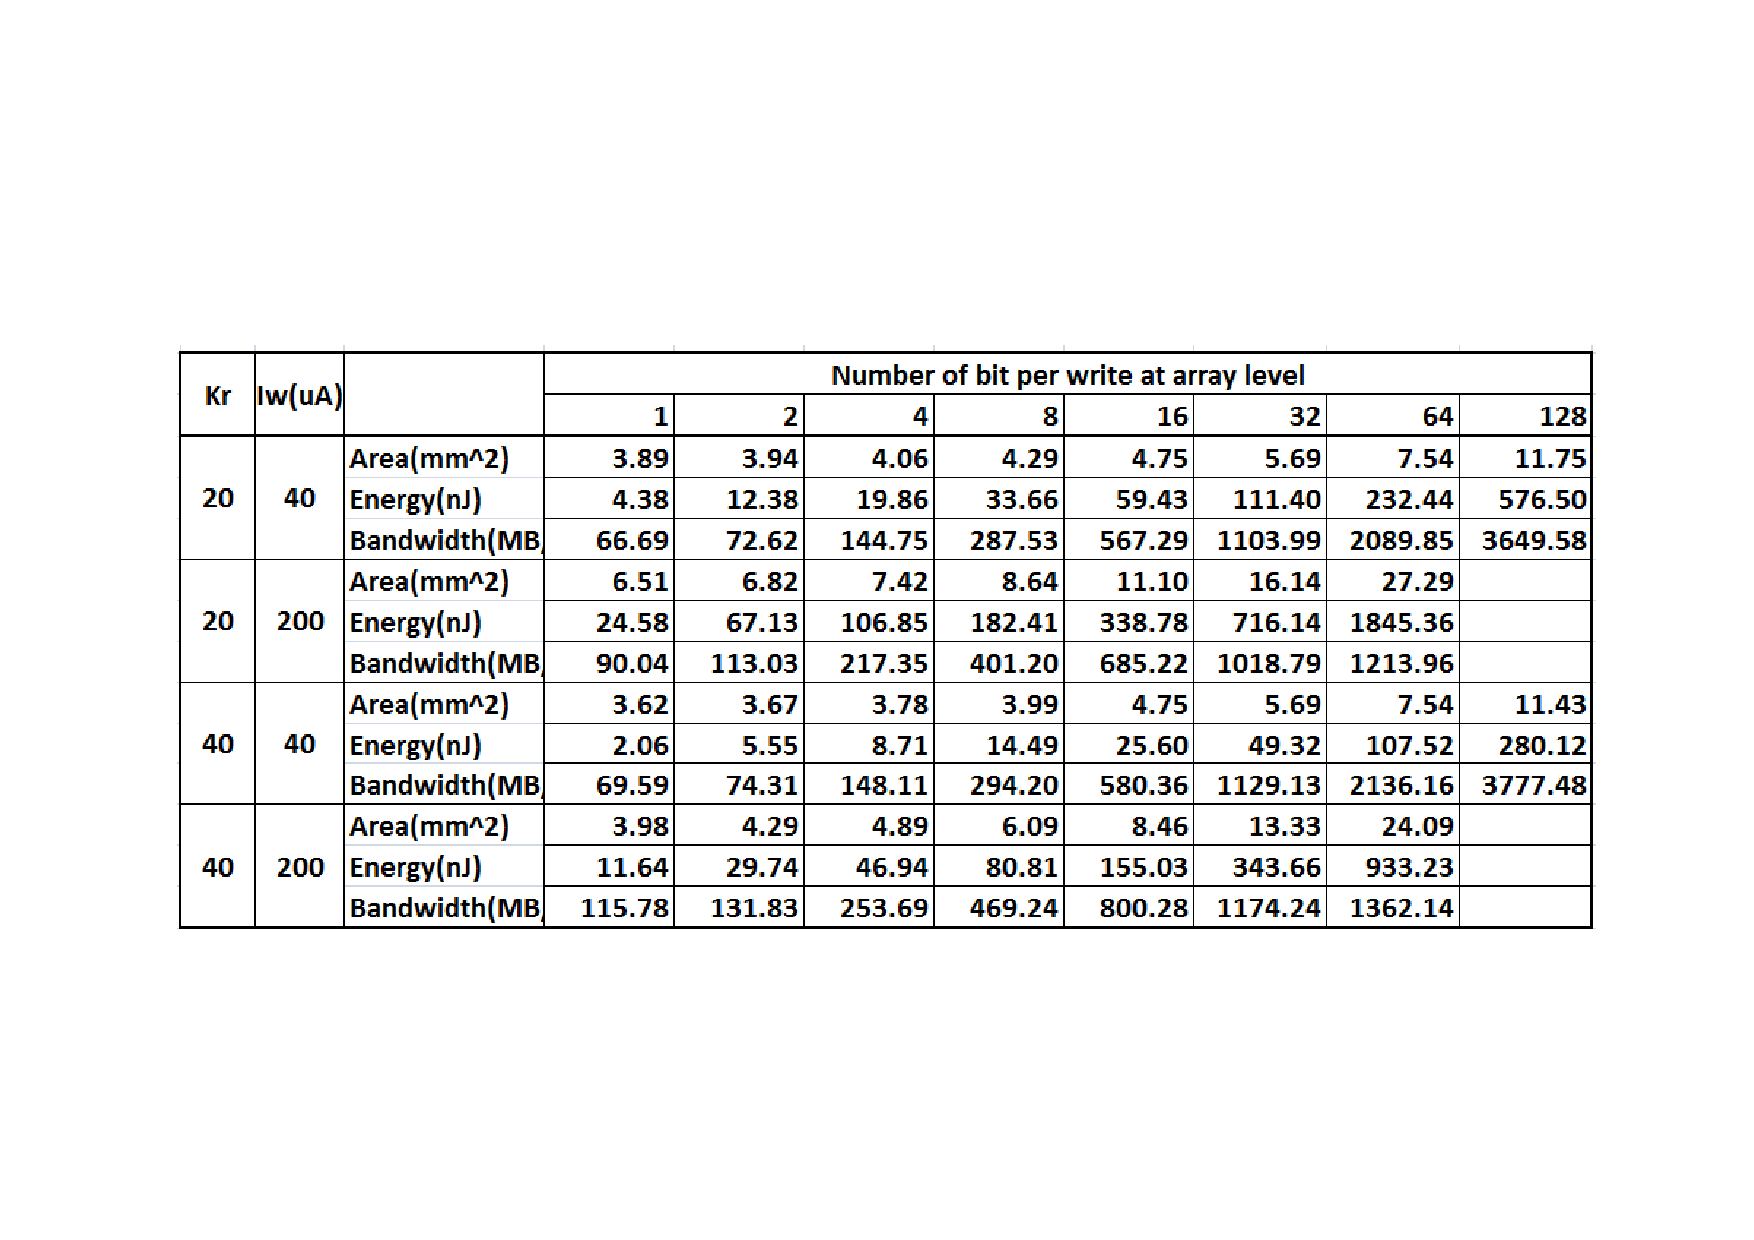
\includegraphics[width=0.5\textwidth]{./figures/Table}\\
%  \caption{Area, energy, and bandwidth results of 256 Mbits ReRAM macro.}
%  \vspace{-5pt}
%\end{figure}


%\begin{figure}[!]
%\centering\label{fig:EpJ}
%  % Requires \usepackage{graphicx}
%  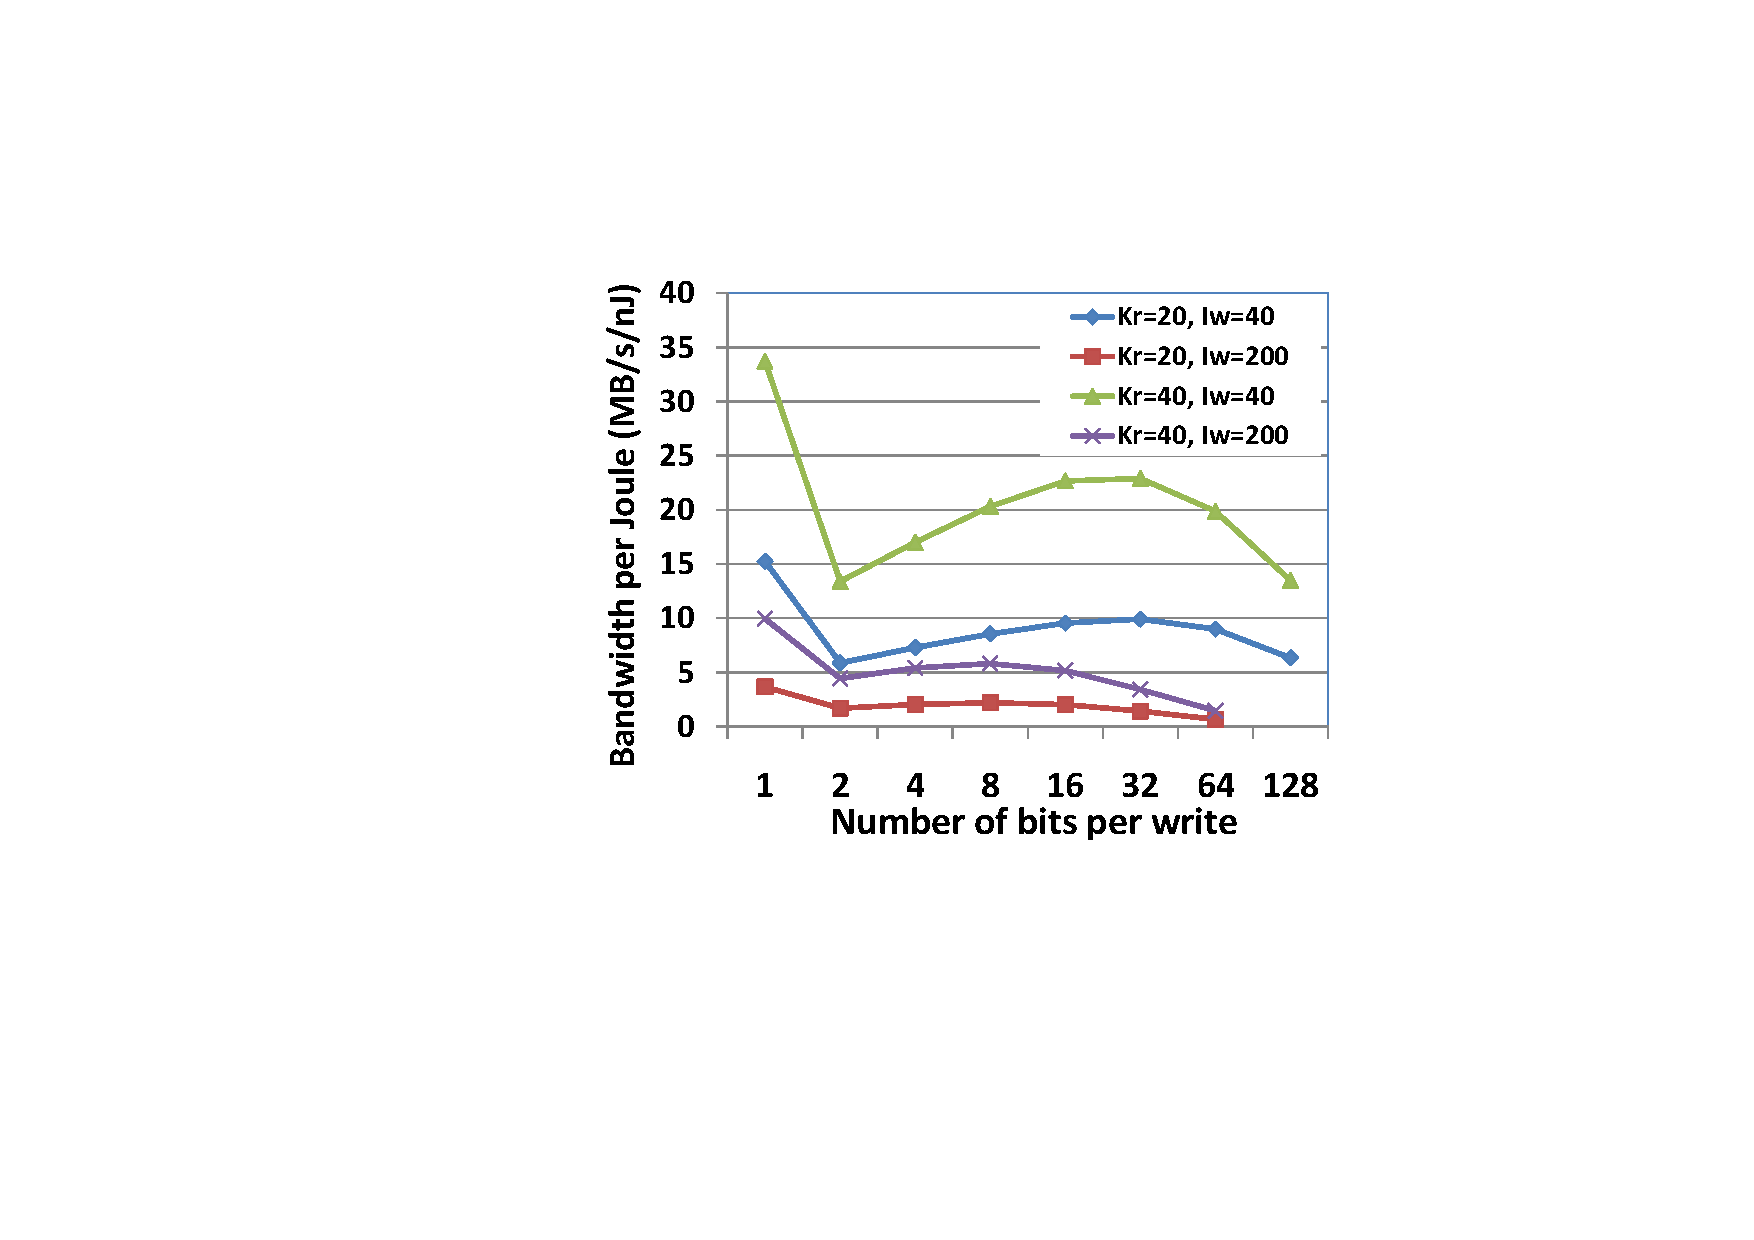
\includegraphics[width=2.3 in]{./figures/EpJ2}\\
%  \caption{Bandwidth-per-Joule of 256 Mbits ReRAM macro.}
%  \vspace{-15pt}
%\end{figure}


\begin{figure}[!]
\centering\label{fig:BWpAE}
  % Requires \usepackage{graphicx}
  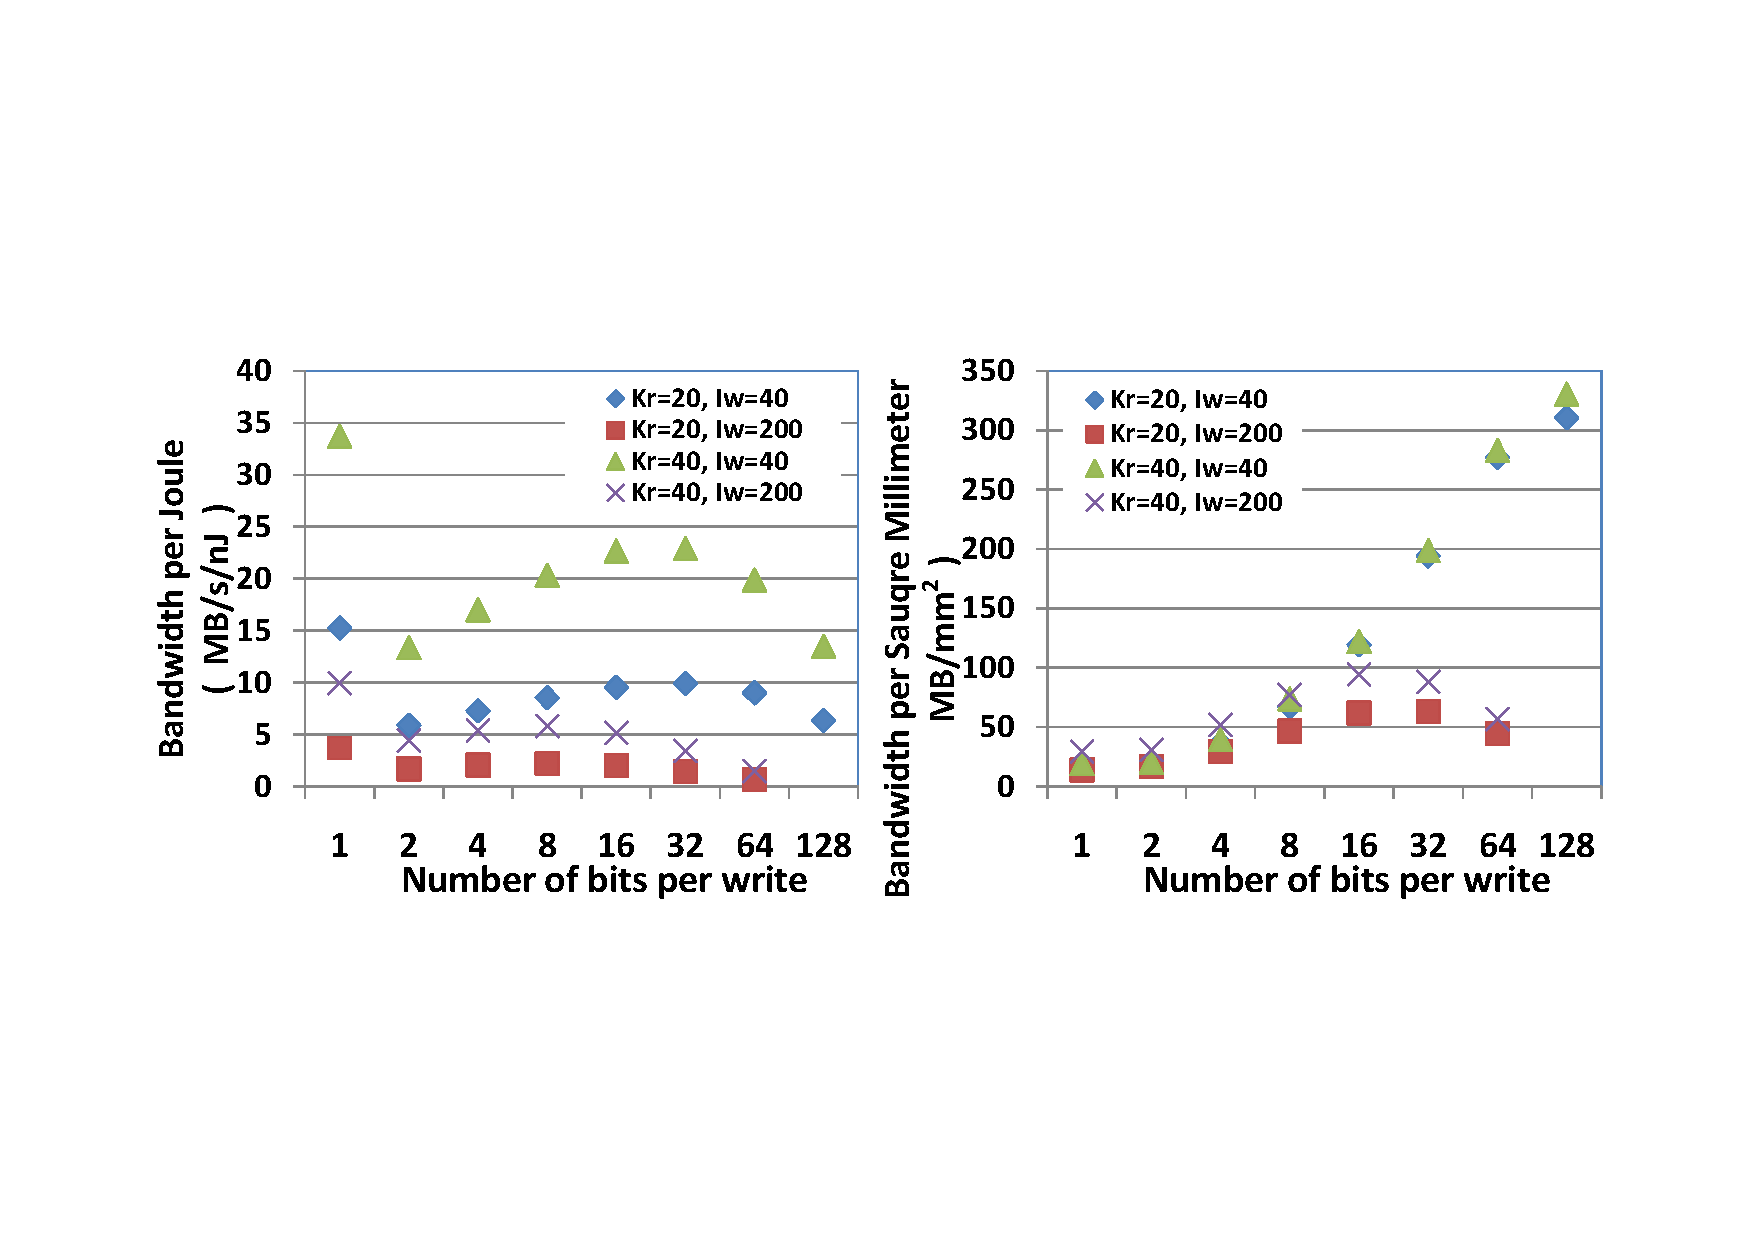
\includegraphics[width=3.4 in]{./figures/BWpAE}\\
  \caption{Bandwidth-per-Joule of 256 Mbits ReRAM macro.}
  \vspace{-5pt}
\end{figure}
\begin{figure}[!]
\centering\label{fig:BWpAE2}
  % Requires \usepackage{graphicx}
  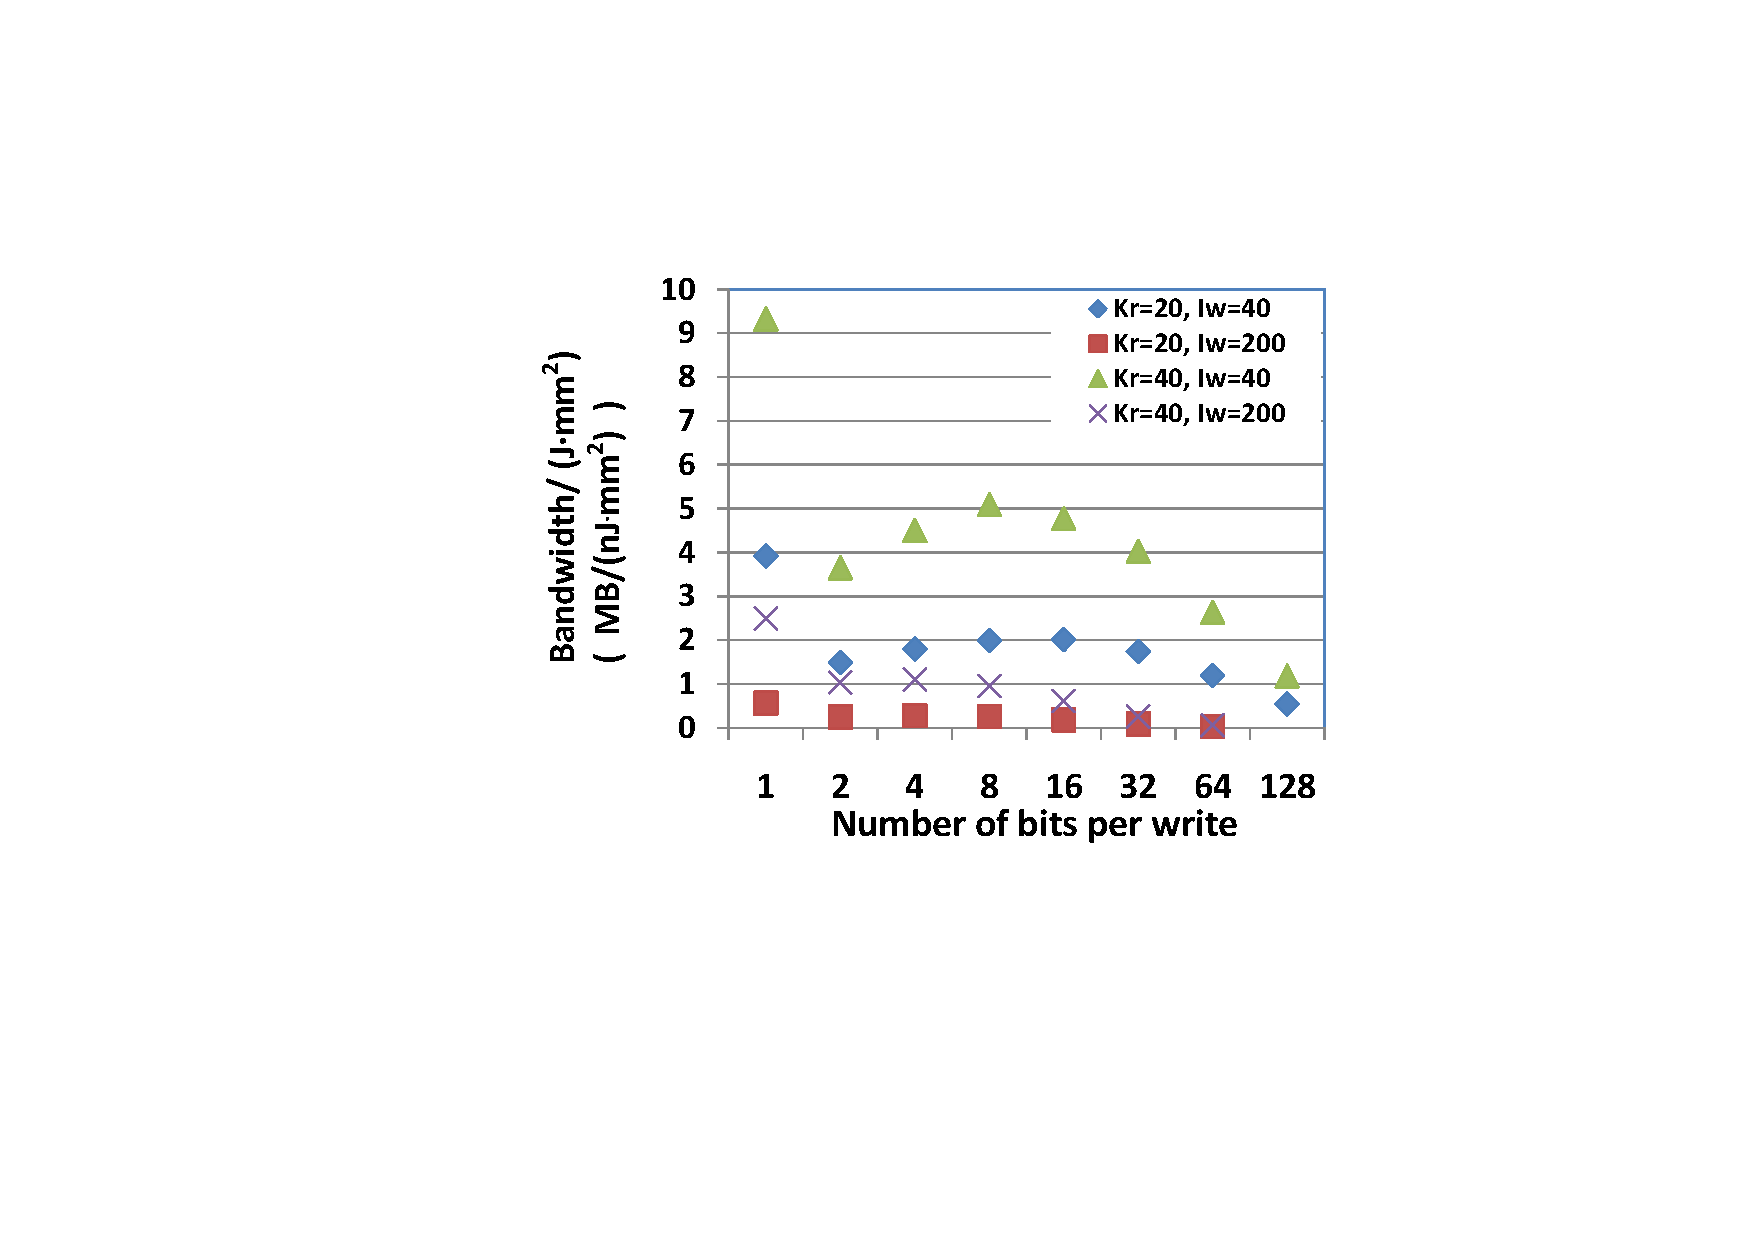
\includegraphics[width=2 in]{./figures/BWpAE2}\\
  \caption{Bandwidth-per-Joule of 256 Mbits ReRAM macro.}
  \vspace{-15pt}
\end{figure}

\vspace{-5pt}
\section{Conclusion}\label{sec:conclusion}
%ReRAM is a promising candidate for next-generation non-volatile memory
%technology. The area efficient cross-point structure is the most
%attractive memory organization for ReRAM memories. However, problems
%inherent in the cross-point structure, such as the existence of sneak
%current and voltage drops along the wires introduce challenges to the
%design of reliable ReRAM cross-point memory arrays.
In this paper, we use a mathematical model to study in detail how
reliability affects the array organization, size, energy consumption, and
area overheads of cross-point arrays. The simulation results show that
multi-bit write operation is more energy efficient than single-bit write
operation, and therefore is more suitable for energy-constrained design.
However, for an area-constrained design, single-bit write operation is
better. Besides, we point out that both increasing nonlinearity and
scaling of write current of the ReRAM cell can reduce the energy
consumption and area overhead significantly, and it is favorable for
large, energy efficient ReRAM design. According to our macro-level
analysis, we figure out that we have to either sacrifice the area
efficiency or increase the energy budget to improve the bandwidth of the
ReRAM macro. In addition, for different optimization target (bandwidth per
nanojoule, bandwidth per square millimeter, and bandwidth per nanojoule),
a optimal number of bits per write exists.

\vspace{-1pt}

\bibliographystyle{ieeetran}
%\begin{scriptsize}
\bibliography{./bib/crossbar,./bib/memristor,./bib/mis,./bib/ReRAM}
%\end{scriptsize}
%\vspace{5pt}
%\end{spacing}
%\end{scriptsize}
%\vspace{10pt}
%\appendix[\vspace{10pt}Details of ReRAM Cross-Point Modeling]
%\vspace{10pt}
%\label{sec:app}

As mentioned in Section~\ref{sec:model}, the model is built upon KCL,
therefore, the current equations for each cross-point can be set following
\begin{equation}\label{equ:KCL0}
 {\Sigma}_{I=1}^kI_k=0.
\end{equation}
For the sake of brevity, we assume that the wordline voltage drivers are
only located at the edge of $V_{W1} \sim V_{Wm}$ and bitline multiplexors
or are located at the edge of $V_{B1} \sim V_{Bn}$. Points located at the
other two edges are left floating.

First of all, for normal points which are located inside the memory array,
the KCL equations take the form of
\begin{equation}\label{equ:KCL1}
R_l^{-1}V_{i,j-1} -(2R_l^{-1}+R_{i,j}^{-1})V_{i,j}+ R_l^{-1}V_{i,j+1}+R_{i,j}^{-1}V'_{i,j}=0,
\end{equation}
for the node at wordline layer and
\begin{equation}\label{equ:KCL2}
R_l^{-1}V'_{i-1,j} -(2R_l^{-1}+R_{i,j}^{-1})V'_{i,j}+ R_l^{-1}V'_{i+1,j}+R_{i,j}^{-1}V_{i,j}=0,
\end{equation}
for all of the nodes with $1<i<m$ and $1<j<n$ in a $m \times n$ array.

For all of the points $V_{i,1}$ ($1\leq i\leq m$) according to different
write schemes, they can be connected to the voltage driver $V_{Wi}$ (as
activated points) or left floating (as floating points). For activated
points, we have
\begin{equation}\label{equ:KCL3}
 -(R_v^{-1}+R_l^{-1}+R_{i,1}^{-1})V_{i,1}+ R_l^{-1}V_{i,2}+R_{i,1}^{-1}V'_{i,1}=-R_v^{-1}V_{Wi},
\end{equation}
and for floating points, we have
\begin{equation}\label{equ:KCL4}
 -(R_l^{-1}+R_{i,1}^{-1})V_{i,1}+ R_l^{-1}V_{i,2}+R_{i,j}^{-1}V'_{i,1}=0.
\end{equation}

Similarly, for the points of $V'_{1,j}$ ($1\leq j\leq n$), the KCL
equations take the form of
\begin{equation}\label{equ:KCL5}
 -(R_s^{-1}+R_l^{-1}+R_{1,j}^{-1})V'_{1,j}+ R_l^{-1}V'_{2,j}+R_{1,j}^{-1}V_{1,j}=-R_s^{-1}V_{Bj},
\end{equation}
for activated points and
\begin{equation}\label{equ:KCL6}
 -(R_l^{-1}+R_{1,j}^{-1})V'_{1,j}+ R_l^{-1}V'_{2,j}+R_{1,j}^{-1}V_{1,j}=0.
\end{equation}
for floating points.

Finally, all of the other points at $V_{i,n}$ and $V'_{m,j}$ ($1\leq i\leq
m, 1\leq j\leq n$) are floating points and have the form of
\begin{equation}\label{equ:KCL7}
 -(R_l^{-1}+R_{i,n}^{-1})V_{i,n}+ R_l^{-1}V_{i,n-1}+R_{i,n}^{-1}V'_{i,n}=0,
\end{equation}
\begin{equation}\label{equ:KCL8}
 -(R_l^{-1}+R_{m,j}^{-1})V'_{m,j}+ R_l^{-1}V'_{m-1,j}+R_{m,j}^{-1}V_{m,j}=0.
\end{equation}

Then, for clarity, a ${2mn\times 1}$ vector ${V}$ is defined to represent
all of the variables in the KCL equations:
\begin{equation}\label{equ:V1}
{V}=[{V_1}^T,{V_2}^T...{V_m}^T,{V'_1}^T,{V'_2}^T...{V'_m}^T]^T,
\end{equation}
where,
%\begin{equation}\label{equ:V2}
%{V_i} = [V_{i,1},V_{i,2}...V_{i,n}]^T,\\
%\end{equation}
%\begin{equation}\label{equ:V3}
%{V'_i} = [V'_{i,1},V'_{i,2}...V'_{i,n}]^T,
%\end{equation}
\begin{equation}\label{equ:V2}
{V_i} = [V_{i,1},V_{i,2}...V_{i,n}]^T,~~{V'_i} = [V'_{i,1},V'_{i,2}...V'_{i,n}]^T,
\end{equation}
for $i=1,2...m$. Then all of the KCL equations can be considered as a
system of linear equations, which has the form
\begin{equation}\label{equ:matrix}
A\cdot V = C.
\end{equation}
$A$ is a ${2mn\times{2mn}}$ coefficient matrix, which is determined by
Equations(\ref{equ:KCL1})-(\ref{equ:KCL8}). $C$ is a ${2mn\times{1}}$
vector, containing the constant terms of these equations. Obviously, the
KCL equation for each point has a relatively simple structure and they are
similar to each other. Thus, the linear equation system has a fixed format
and simple structure, which is easy to establish and adjust according to
different design schemes and cell parameters. Moreover, matrix $A$ is
populated primarily with zeros and can be saved as a sparse matrix, which
will further reduce the storage cost during the computation.

The characteristics of the linear system can be summarized as
\begin{enumerate}
  \item As shown in Equation~(\ref{equ:blockedmatrix}), the
      coefficient matrix $A$ can be further partitioned into four
      subblocks
    \begin{equation}\label{equ:blockedmatrix}
        \mathbf{A} = \left[
        \begin{array}{cc}
            A1 & A2  \\
            A3 & A4  \\
        \end{array} \right].
    \end{equation}
All of these subblocks have the same size of $mn\times mn$. Subblock
$A2$ and $A3$ are diagonal matrixes and have the same form of
%\begin{equation}\label{equ:A2A3}
%        A2 = A3 = \left[
%        \begin{array}{cccc}
%            R_{1,1}^{-1}    & 0             & \ldots    & 0 \\
%            0               & R_{2,2}^{-1}  & \ddots    & \vdots  \\
%            \vdots          & \ddots        & \ddots    & 0 \\
%            0               & \ldots        & 0         & R_{mn,mn}^{-1} \\
%        \end{array} \right].
%    \end{equation}
\begin{equation}\label{equ:A2A3}
        A2 = A3 = \left[
        \begin{array}{ccccccc}
            R_{1,1}^{-1}    & 0             & 0             & ~         & \ldots    & ~             & 0    \\
            0               & \ddots        & 0             & ~         & ~         & ~             & ~    \\
            0               & 0             & R_{1,n}^{-1}  & ~         & \ddots    & ~             & \vdots    \\
            ~               & ~             & ~             & \ddots    & ~         & ~             & ~    \\
            \vdots          & ~        & \ddots             & ~         & R_{m,1}^{-1}    & 0       & 0   \\
            ~               & ~             & ~             & ~         & 0         & \ddots        & 0    \\
            0               & 0             & \ldots              & ~         & 0    & 0             & R_{m,n}^{-1}    \\

        \end{array} \right].
\end{equation}
$A2$ and $A3$ do not change their values with different schemes.

However, $A1$ and $A4$ are a little more complex than $A2$ and $A3$.
$A1$ is a tridiagonal matrix and has nonzero elements only located in
the main diagonal, and the first line below and above the diagonal.
Similarly, $A4$ is a special tridiagonal matrix, which has nonzero
elements in the main diagonal, and the $n^{th}$ line below and above
the diagonal, where $n$ is the number of bitlines in the cross-point
model. The coefficients of normal points in $A1$ and $A4$ can be
easily derived from Equation (\ref{equ:KCL1}) and (\ref{equ:KCL2}) as

\begin{equation}\label{equ:A12}
\left\{
    \begin{array}{ll}
    A1(k,k-1) = R_l^{-1}\\
    A1(k,k)~~~~~ = -(2R_l^{-1}+R_{i,j}^{-1})~~~~,\\
    A1(k,k+1) = R_l^{-1}\\
    \end{array} \right.
    \end{equation}

and
\begin{equation}\label{equ:A122}
\left\{
    \begin{array}{ll}
    A4(k,k-n) = R_l^{-1}\\
    A4(k,k)~~~~~ = -(2R_l^{-1}+R_{i,j}^{-1})~~~~,\\
    A4(k,k+n) = R_l^{-1}\\
    \end{array} \right.
    \end{equation}
where $ k=(i-1)n+j$, $1<i<m$, and $1<j<n$.

However, since the edge conditions vary with different program
schemes, the coefficients of points at the edge of the array may be
different. Clearly, the four edges shown in Figure~\ref{fig:modeling}
correspond to different coefficients in $A1$ and $A4$. Therefore,
after initializing matrix $A1$ and $A4$ following
Equations(\ref{equ:A12}) and (\ref{equ:A122}), the coefficients
related to edge points should be updated to proper value according to
the program schemes. Take the nodes at the left edge of the array
($V_{i,1}, 1\leq i \leq n$) as an example. All of the coefficients
related to these nodes are located in $A1$, which should be set as

    \begin{equation}
    A1(k,k) = \left\{
    \begin{array}{ll}
    -(R_l^{-1}+R_{i,1}^{-1})   & \text{if } floating\\
    -(R_v^{-1}+R_l^{-1}+R_{i,1}^{-1})& \text{if } activated
    \end{array} \right.
    \end{equation}
    where $k=(n-1)i+1$ for $1\leq i\leq m$.

Similar procedures can be performed to initiate the coefficients
related to other edges.

\item The constant term $C$ is a $2mn{\times}1$ vector.
    Equation(\ref{equ:KCL1})-(\ref{equ:KCL8}) show that only KCL
    equations of the activated points have constant terms. Therefore,
    only the following elements in $C$ may have non-zero value:
    $C((i-1)n+1)$, $C(in)$, $C(mn+i)$ and $C((2m-1)n+i)$ for
    $i=1,2...m$, corresponding to the nodes at the four edges
    respectively. If the wordline is driven from one side, only nodes
    $V_{i,1}$ and $V_{1,j}$ can be activated. Therefore, the constant
    corresponding to these nodes can be defined as
\begin{equation}
    C((i-1)n+1) = \left\{
    \begin{array}{ll}
    0   & \text{if } floating\\
    -R_v^{-1}V_{Wi}& \text{if } activated
    \end{array} \right.
    \end{equation}
for wordline layer and
\begin{equation}
    C(mn+j) = \left\{
    \begin{array}{ll}
    0   & \text{if } floating\\
    -R_s^{-1}V_{Bj}& \text{if } activated
    \end{array} \right.
    \end{equation}
for bitline layer, with $1\leq i\leq m$, and $1\leq j\leq n$.
\end{enumerate}


\end{document}
